% ******************************* PhD Thesis Template **************************
% Please have a look at the README.md file for info on how to use the template

\documentclass[a4paper,12pt,times,numbered,print,index]{PhDThesisPSnPDF}

% ******************************************************************************
% ******************************* Class Options ********************************
% *********************** See README for more details **************************
% ******************************************************************************

% `a4paper'(The University of Cambridge PhD thesis guidelines recommends a page
% size a4 - default option) or `a5paper': A5 Paper size is also allowed as per
% the Cambridge University Engineering Deparment guidelines for PhD thesis
%
% `11pt' or `12pt'(default): Font Size 10pt is NOT recommended by the University
% guidelines
%
% `oneside' or `twoside'(default): Printing double side (twoside) or single
% side.
%
% `print': Use `print' for print version with appropriate margins and page
% layout. Leaving the options field blank will activate Online version.
%
% `index': For index at the end of the thesis
%
% `draftclassic': For draft mode without loading any images (same as draft in book)
%
% `draft': Special draft mode with line numbers, images, and water mark with
% timestamp and custom text. Position of the text can also be modified.
%
% `abstract': To generate only the title page and abstract page with
% dissertation title and name, to submit to the Student Registry
%
% `chapter`: This option enables only the specified chapter and it's references
%  Useful for review and corrections.
%
% ************************* Custom Page Margins ********************************
%
% `custommargin`: Use `custommargin' in options to activate custom page margins,
% which can be defined in the preamble.tex. Custom margin will override
% print/online margin setup.
%
% *********************** Choosing the Fonts in Class Options ******************
%
% `times' : Times font with math support. (The Cambridge University guidelines
% recommend using times)
%
% `fourier': Utopia Font with Fourier Math font (Font has to be installed)
%            It's a free font.
%
% `customfont': Use `customfont' option in the document class and load the
% package in the preamble.tex
%
% default or leave empty: `Latin Modern' font will be loaded.
%
% ********************** Choosing the Bibliography style ***********************
%
% `authoryear': For author-year citation eg., Krishna (2013)
%
% `numbered': (Default Option) For numbered and sorted citation e.g., [1,5,2]
%
% `custombib': Define your own bibliography style in the `preamble.tex' file.
%              `\RequirePackage[square, sort, numbers, authoryear]{natbib}'.
%              This can be also used to load biblatex instead of natbib
%              (See Preamble)
%
% **************************** Choosing the Page Style *************************
%
% `default (leave empty)': For Page Numbers in Header (Left Even, Right Odd) and
% Chapter Name in Header (Right Even) and Section Name (Left Odd). Blank Footer.
%
% `PageStyleI': Chapter Name next & Page Number on Even Side (Left Even).
% Section Name & Page Number in Header on Odd Side (Right Odd). Footer is empty.
%
% `PageStyleII': Chapter Name on Even Side (Left Even) in Header. Section Number
% and Section Name in Header on Odd Side (Right Odd). Page numbering in footer

% Uncomment to change page style
%\pagestyle{PageStyleII}

% ********************************** Preamble **********************************
% Preamble: Contains packages and user-defined commands and settings
% ******************************************************************************
% ****************************** Custom Margin *********************************

% Add `custommargin' in the document class options to use this section
% Set {innerside margin / outerside margin / topmargin / bottom margin}  and
% other page dimensions
\ifsetCustomMargin
  \RequirePackage[left=37mm,right=30mm,top=35mm,bottom=30mm]{geometry}
  \setFancyHdr % To apply fancy header after geometry package is loaded
\fi

% Add spaces between paragraphs
%\setlength{\parskip}{0.5em}
% Ragged bottom avoids extra whitespaces between paragraphs
\raggedbottom
% To remove the excess top spacing for enumeration, list and description
%\usepackage{enumitem}
%\setlist[enumerate,itemize,description]{topsep=0em}

% *****************************************************************************
% ******************* Fonts (like different typewriter fonts etc.)*************

% Add `customfont' in the document class option to use this section

%\ifsetCustomFont
  % Set your custom font here and use `customfont' in options. Leave empty to
  % load computer modern font (default LaTeX font).
  %\RequirePackage{helvet}

  % For use with XeLaTeX
%    \setmainfont[
%      Path              = ./libertine/opentype/,
%      Extension         = .otf,
%      UprightFont = LinLibertine_R,
%      BoldFont = LinLibertine_RZ, % Linux Libertine O Regular Semibold
%      ItalicFont = LinLibertine_RI,
%      BoldItalicFont = LinLibertine_RZI, % Linux Libertine O Regular Semibold Italic
%    ]
%    {libertine}
%    % load font from system font
%    \newfontfamily\libertinesystemfont{Linux Libertine O}
%\fi

\usepackage{libertine}
\usepackage{libertinust1math}
\usepackage[T1]{fontenc}


% *****************************************************************************
% **************************** Custom Packages ********************************

% ************************* Algorithms and Pseudocode **************************

%\usepackage{algpseudocode}


% ********************Captions and Hyperreferencing / URL **********************

% Captions: This makes captions of figures use a boldfaced small font.
%\RequirePackage[small,bf]{caption}

\RequirePackage[labelsep=space,tableposition=top]{caption}
\renewcommand{\figurename}{Fig.} %to support older versions of captions.sty


% *************************** Graphics and figures *****************************

%\usepackage{rotating}
%\usepackage{wrapfig}

% Uncomment the following two lines to force Latex to place the figure.
% Use [H] when including graphics. Note 'H' instead of 'h'
%\usepackage{float}
%\restylefloat{figure}

% Subcaption package is also available in the sty folder you can use that by
% uncommenting the following line
% This is for people stuck with older versions of texlive
%\usepackage{sty/caption/subcaption}
\usepackage{subcaption}

% ********************************** Tables ************************************
\usepackage{booktabs} % For professional looking tables
\usepackage{multirow}

%\usepackage{multicol}
%\usepackage{longtable}
%\usepackage{tabularx}


% *********************************** SI Units *********************************
\usepackage{siunitx} % use this package module for SI units


% ******************************* Line Spacing *********************************

% Choose linespacing as appropriate. Default is one-half line spacing as per the
% University guidelines

% \doublespacing
% \onehalfspacing
% \singlespacing


% ************************ Formatting / Footnote *******************************

% Don't break enumeration (etc.) across pages in an ugly manner (default 10000)
%\clubpenalty=500
%\widowpenalty=500

%\usepackage[perpage]{footmisc} %Range of footnote options


% *****************************************************************************
\usepackage[ruled,vlined]{algorithm2e}
\usepackage{bbold}
\usepackage{amssymb}
\usepackage{amsmath}
\usepackage{float}
%\usepackage{subfig}
\usepackage{graphicx}
\usepackage{soul}
\usepackage{pdfpages}
\usepackage{booktabs} % Tables
\usepackage{pifont}
\usepackage{placeins}
\usepackage{afterpage}




% *************************** Bibliography  and References ********************

%\usepackage{cleveref} %Referencing without need to explicitly state fig /table

% Add `custombib' in the document class option to use this section
\ifuseCustomBib
   \RequirePackage[square, sort, numbers, authoryear]{natbib} % CustomBib

% If you would like to use biblatex for your reference management, as opposed to the default `natbibpackage` pass the option `custombib` in the document class. Comment out the previous line to make sure you don't load the natbib package. Uncomment the following lines and specify the location of references.bib file

%\RequirePackage[backend=biber, style=numeric-comp, citestyle=numeric, sorting=nty, natbib=true]{biblatex}
%\addbibresource{References/references} %Location of references.bib only for biblatex, Do not omit the .bib extension from the filename.

\fi

% changes the default name `Bibliography` -> `References'
\renewcommand{\bibname}{References}


% ******************************************************************************
% ************************* User Defined Commands ******************************
% ******************************************************************************

% *********** To change the name of Table of Contents / LOF and LOT ************

%\renewcommand{\contentsname}{My Table of Contents}
%\renewcommand{\listfigurename}{My List of Figures}
%\renewcommand{\listtablename}{My List of Tables}


% ********************** TOC depth and numbering depth *************************

\setcounter{secnumdepth}{2}
\setcounter{tocdepth}{2}


% ******************************* Nomenclature *********************************

% To change the name of the Nomenclature section, uncomment the following line

%\renewcommand{\nomname}{Symbols}


% ********************************* Appendix ***********************************

% The default value of both \appendixtocname and \appendixpagename is `Appendices'. These names can all be changed via:

%\renewcommand{\appendixtocname}{List of appendices}
%\renewcommand{\appendixname}{Appndx}

% *********************** Configure Draft Mode **********************************

% Uncomment to disable figures in `draft'
%\setkeys{Gin}{draft=true}  % set draft to false to enable figures in `draft'

% These options are active only during the draft modeLatin Modern 
% Default text is "Draft"
%\SetDraftText{DRAFT}

% Default Watermark location is top. Location (top/bottom)
%\SetDraftWMPosition{bottom}

% Draft Version - default is v1.0
%\SetDraftVersion{v1.1}

% Draft Text grayscale value (should be between 0-black and 1-white)
% Default value is 0.75
%\SetDraftGrayScale{0.8}


% ******************************** Todo Notes **********************************
%% Uncomment the following lines to have todonotes.

%\ifsetDraft
%	\usepackage[colorinlistoftodos]{todonotes}
%	\newcommand{\mynote}[1]{\todo[author=kks32,size=\small,inline,color=green!40]{#1}}
%\else
%	\newcommand{\mynote}[1]{}
%	\newcommand{\listoftodos}{}
%\fi

% Example todo: \mynote{Hey! I have a note}

% ******************************** Highlighting Changes **********************************
%% Uncomment the following lines to be able to highlight text/modifications.
%\ifsetDraft
%  \usepackage{color, soul}
%  \newcommand{\hlc}[2][yellow]{{\sethlcolor{#1} \hl{#2}}}
%  \newcommand{\hlfix}[2]{\texthl{#1}\todo{#2}}
%\else
%  \newcommand{\hlc}[2]{}
%  \newcommand{\hlfix}[2]{}
%\fi

% Example highlight 1: \hlc{Text to be highlighted}
% Example highlight 2: \hlc[green]{Text to be highlighted in green colour}
% Example highlight 3: \hlfix{Original Text}{Fixed Text}

% *****************************************************************************
% ******************* Better enumeration my MB*************
\usepackage{enumitem}


% ************************ Thesis Information & Meta-data **********************
% Thesis title and author information, refernce file for biblatex
% ************************ Thesis Information & Meta-data **********************
%% The title of the thesis
\title{Optimal Importance Sampling in Quantum Monte Carlo for Lattice Models}
%\texorpdfstring is used for PDF metadata. Usage:
%\texorpdfstring{LaTeX_Version}{PDF Version (non-latex)} eg.,
%\texorpdfstring{$sigma$}{sigma}

%% Subtitle (Optional)
%\subtitle{Using the CUED template}

%% The full name of the author
\author{Bla\v z Stojanovi\v c}

%% Department (eg. Department of Engineering, Maths, Physics)
\dept{Department of Physics}

%% University and Crest
\university{University of Cambridge}
% Crest minimum should be 30mm.
%\crest{
\includegraphics[width=0.2\textwidth]{University_Crest}}
%% Use this crest, if you are using the college crest
%% Crest long miminum should be 65mm
\crest{
\includegraphics[width=0.45\textwidth]{University_Crest_Long}}

%% College shield [optional] 
% Crest minimum should be 30mm.
\collegeshield{
\includegraphics[width=0.2\textwidth]{Figs/CollegeShields/StJohns}}


%% Supervisor (optional)
%% for multiple supervisors, append each supervisor with the \newline command
\supervisor{Prof. A. Lamacraft}

%% Supervisor Role (optional) - Supervisor (default) or advisor
% \supervisorrole{\textbf{Supervisors: }}
%% if no title is desired:
% \supervisorrole{}

%% Supervisor line width: required to align supervisors
%\supervisorlinewidth{0.35\textwidth}

%% Advisor (optional)
%% for multiple advisors, append each advisor with the \newline command
%\advisor{Dr. A. Advisor\newline
%Dr. B. Advisor}
     
%% Advisor Role (optional) - Advisor (default) or leave empty
% \advisorrole{Advisors: }
%% if no title is required
% \advisorrole{}

%% Advisor line width: required to align supervisors
%\advisorlinewidth{0.25\textwidth}


%% You can redefine the submission text:
% Default as per the University guidelines:
% ``This dissertation is submitted for the degree of''
%\renewcommand{\submissiontext}{change the default text here if needed}

%% Full title of the Degree
\degreetitle{Master of Philosophy in Scientific Computing}

%% College affiliation (optional)
\college{St. John's College}

%% Submission date
% Default is set as {\monthname[\the\month]\space\the\year}
%\degreedate{September 2014} 

%% Meta information
\subject{LaTeX} \keywords{{LaTeX} {PhD Thesis} {Engineering} {University of
Cambridge}}


% ***************************** Abstract Separate ******************************
% To printout only the titlepage and the abstract with the PhD title and the
% author name for submission to the Student Registry, use the `abstract' option in
% the document class.

\ifdefineAbstract
 \pagestyle{empty}
 \includeonly{Declaration/declaration, Abstract/abstract}
\fi

% ***************************** Chapter Mode ***********************************
% The chapter mode allows user to only print particular chapters with references
% Title, Contents, Frontmatter are disabled by default
% Useful option to review a particular chapter or to send it to supervisior.
% To use choose `chapter' option in the document class

\ifdefineChapter
 \includeonly{Chapter3/chapter3}
\fi

% ******************************** Front Matter ********************************
\begin{document}

\frontmatter

\maketitle

% ******************************* Thesis Dedidcation ********************************

\begin{dedication} 

To my family.

\end{dedication}


% ******************************* Thesis Declaration ***************************

\begin{declaration}

This dissertation is substantially my own work and conforms to the University of Cambridge’s guidelines on plagiarism. Where reference has been made to other research this is acknowledged in the text and bibliography. This dissertation contains fewer than 15,000 words including appendices, figure legends, and tables.

\end{declaration}


% ************************** Thesis Acknowledgements **************************

\begin{acknowledgements}      


And I would like to acknowledge ...


\end{acknowledgements}
s
% ************************** Thesis Abstract *****************************
% Use `abstract' as an option in the document class to print only the titlepage and the abstract.
\begin{abstract}
	
This is where you write your abstract ...

\end{abstract}


% *********************** Adding TOC and List of Figures ***********************

\tableofcontents

\listoffigures

\listoftables

% \printnomenclature[space] space can be set as 2em between symbol and description
%\printnomenclature[3em]

\printnomenclature

% ******************************** Main Matter *********************************
\mainmatter

%!TEX root = ../thesis.tex
%*******************************************************************************
%*********************************** First Chapter *****************************
%*******************************************************************************

\chapter{Introduction}  %Title of the First Chapter
\label{chapter1}

\ifpdf
\graphicspath{{Chapter1/Figs/Raster/}{Chapter1/Figs/PDF/}{Chapter1/Figs/}}
\else
\graphicspath{{Chapter1/Figs/Vector/}{Chapter1/Figs/}}
\fi


%********************************** %Chapter 1 Nomenclature **************************************
\nomenclature[z-ml]{ML}{Machine Learning}
\nomenclature[z-dl]{DL}{Deep Learning}
\nomenclature[z-vae]{VAE}{Variational Autoencoder}
\nomenclature[z-gan]{GAN}{General Adversarial Network}
\nomenclature[z-nn]{NN}{Neural Network}
\nomenclature[z-cnn]{CNN}{Convolutional Neural Network}

\nomenclature[z-qmc]{QMC}{Quantum Monte Carlo}
\nomenclature[z-vmc]{VMC}{Variational Quantum Monte Carlo}
\nomenclature[z-dmc]{DMC}{Diffusion Quantum Monte Carlo}
%!TEX root = ../thesis.tex
%*******************************************************************************
%****************************** Second Chapter *********************************
%*******************************************************************************

\chapter{On the quantum many-body problem}
\label{chapter2}

\ifpdf
    \graphicspath{{Chapter2/Figs/Raster/}{Chapter2/Figs/PDF/}{Chapter2/Figs/}}
\else
    \graphicspath{{Chapter2/Figs/Vector/}{Chapter2/Figs/}}
\fi

%********************************** %First Section  **************************************
\section{Lattice models}
\label{sec:lattice-models}

\subsection{Historical introduction}
\label{subsec:latt-hist}
\begin{itemize}
	\item I think starting from the magnetism point of view might be the best way to go, slowly lead into the field of condensed matter theory and lattice models. 
\end{itemize}

\subsection{The Schr{\"o}dinger equation and the Feynman path integral}
\label{subsec:latt-qm}
The wavefunction
\begin{equation}
	\Psi\left(r_{1}, \ldots, r_{N}\right)
\end{equation}
the Schr\" odinger equation
\begin{equation}
	i \frac{\partial \psi(\boldsymbol{r}, t)}{\partial t}= \hat{H} \psi(\textbf{r}, t)
\end{equation}
for a single particle in an external potential $\hat{V}(\boldsymbol{r})$ the Hamiltonian is 
\begin{equation}
	\hat H \phi(\boldsymbol{r})=-\frac{1}{2} \nabla^{2} \phi(\boldsymbol{r})+\hat{V}(\boldsymbol{r}) \phi(\boldsymbol{r}).
\end{equation}
Alternatively to the Schr\" odinger equation one can use an integral Green's function representation to express the wavefunction $\psi$ at some future time $t_2$ given initial condition $\psi(\boldsymbol{r}, t_1)$ as
\begin{equation}
	\psi\left(\boldsymbol{r}_{2}, t_{2}\right)=\int  \mathcal{K}\left(\boldsymbol{r}_{2}, t_{2} ; \boldsymbol{r}_{1}, t_{1}\right) \psi\left(\boldsymbol{r}_{1}, t_{1}\right) \mathrm{d} \boldsymbol{r}_{1}.
\end{equation}
The solution to  equation
\begin{equation}
	\left(i \frac{\partial}{\partial t_{2}}-H_{\boldsymbol{r}_{2}}\right) \mathcal{K}\left(\boldsymbol{r}_{2}, t_{2} ; \boldsymbol{r}_{1}, t_{1}\right)=i \delta\left(\boldsymbol{r}_{1}-\boldsymbol{r}_{2}\right) \delta\left(t_{1}-t_{2}\right)
\end{equation}
and the \textit{propagator} $\mathcal{K}\left(\boldsymbol{r}_{2}, t_{2} ; \boldsymbol{r}_{1}, t_{1}\right)$ is expressed using the Feynman path integral
\begin{equation}
	\label{eq:FPI}
	\mathcal{K}\left(\boldsymbol{r}_{2}, t_{2} ; \boldsymbol{r}_{1}, t_{1}\right)=\int_{\substack{\boldsymbol{r}\left(t_{1}\right)=r_{1} \\ \boldsymbol{r}\left(t_{2}\right)=r_{2}}}  \mathcal{D} \boldsymbol{r}(t) \exp \left(i \int_{t_{1}}^{t_{2}} \mathcal{L}(\boldsymbol{r}, \dot{\boldsymbol{r}}) d t\right),
\end{equation}
where $\mathcal{L}$ is the classical Lagrangian function of the system
\begin{equation}
	L(\boldsymbol{r}, \dot{\boldsymbol{r}})=\frac{1}{2} \dot{\boldsymbol{r}}^{2}-\hat V(\boldsymbol{r}),
\end{equation}
and the integral is over all paths that satisfy the endpoint conditions.

\subsection{Examples of lattice models}
\label{subsec:latt-examples}

\begin{equation}
	\hat{\sigma}^x_{i}=\left(\begin{array}{cc}0 & 1 \\ 1 & 0\end{array}\right)_{i} \quad \hat{\sigma}^y_{i}=\left(\begin{array}{cc}0 & -i \\ i & 0\end{array}\right)_{i} \quad \hat{\sigma}^z_{i}=\left(\begin{array}{cc}1 & 0 \\ 0 & -1\end{array}\right)_{i}
\end{equation}


\subsubsection{Transverse-field Field Ising model}
\begin{equation}
	\hat H_{\mathrm{Ising}}=-J \sum_{\langle i, j\rangle} \hat{\sigma}^z_{i} \hat{\sigma}^z_{j}-h \sum_{i} \sigma^x_{i}
\end{equation}

\subsubsection{Heisenberg model}
\begin{equation}
	\hat{H}_{\mathrm{Heisenberg}}=-\frac{1}{2} \sum_{j=1}^{N}
	\left[J_{x} \hat{\sigma}_{j}^{x} \hat{\sigma}_{j+1}^{x}+J_{y} \hat{\sigma}_{j}^{y} \sigma_{j+1}^{y}+J_{z} \hat{\sigma}_{j}^{z} \hat{\sigma}_{j+1}^{z}+h \hat{\sigma}_{j}^{z}
	\right]
\end{equation}

\subsubsection{Bose-Hubbard model}
\begin{equation}
	\hat{H}_{\mathrm{BH}}= -t \sum_{\langle i, j\rangle} \hat{b}_{i}^{\dagger} \hat{b}_{j}+\frac{U}{2} \sum_{i} \hat{n}_{i}\left(\hat{n}_{i}-1\right)-\mu \sum_{i} \hat{n}_{i}
\end{equation}

%********************************** % ??? Section  *************************************
\newpage
\section{Approaches to the quantum many-body problem}
\label{sec:QMBP}
The quantum many-body problem, which amounts to solving the $3N$-dimensional Schr\"odinger equation, underpins a large part of quantum chemistry, condensed matter physics and materials science. The problem is notoriously hard to solve and very few systems with analytical solutions exist, most of them constrained in some artificial way such that they lend themselves to mathematical analysis. Examples include the Hookium atom, an analogue of helium where two electrons interact with the nucleus via a Hookean potential, Spherium, a system of two electrons confined to the surface of a sphere, and the Luttinger liquid of fermions in a one-dimensional conductor. Great efforts have been made in the nearly 100 years since the conception of the Schr\" odinger equation, in developing both analytical and numerical techniques to produce insights into quantum systems. Perhaps the most impactful was the development of various approximate methods that solve the many-body problem with our limited computational resources. While there is ongoing work on quantum simulators and computers that could greatly speed-up solving quantum problems~\cite{feynman2018simulating, childs2010relationship}, we here discuss methods one can use with a classical computer. The commonality of all mentioned methods is that they try to tame the exponential growth of the underlying Hilbert space w.r.t the system size, they differ in how they achieve this. The three most common assumptions/simplifications to the many-body problem employed in condensed matter and quantum chemistry are the Born-Oppenheimer approximation, that electronic motion is instantaneous compared to the nuclear motion, the use of chemical basis sets, which transforms the PDE into an algebraic problem, and usually neglecting relativistic effects.
%\begin{figure}[h]
%	\centering
%	\subfloat{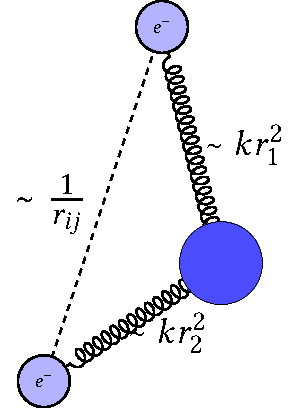
\includegraphics[width=0.3\linewidth]{Chapter2/Figs/Vector/hookium_diagram.pdf}}
%	\qquad\qquad\qquad
%	\subfloat{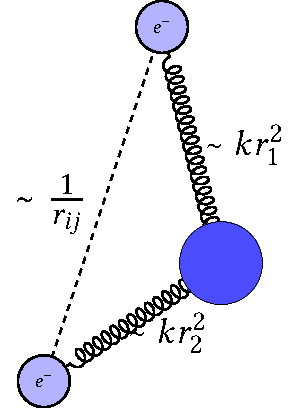
\includegraphics[width=0.3\linewidth]{Chapter2/Figs/Vector/hookium_diagram.pdf}}
%	\caption[Hookium and Spherium]{\textbf{Hookium and Spherium.}}
%	\label{fig:qmbp-hookium_and_spherium}
%\end{figure}

\subsubsection{Hartree-Fock}
One of the most common approaches to the many-body problem is to replace the original interacting many-body problem with a set of independent-particle problems with effective potential. \textbf{Hartree-Fock} (HF) approaches solve an auxiliary system of independent electrons in a self-consistent field and assume that the wave function (for fermions) can be represented as a single Slater determinant. The HF method does not include electron correlation, which makes it a good approximation only in systems where correlation contributions are small. 

\subsubsection{Post-Hartree-Fock methods}
Post-HF methods, such as Coupled Cluster, Configuration interaction and M\o ller-Plesset theory include correlation by considering a linear combination of Slater determinants. They can be extremely accurate but come at a high computational cost. 

\subsubsection{Density Funcitonal Theory}
Alternatively \textbf{Density Functional Theory} (DFT) reformulates the many-body electron problem in terms of the $3$-dimensional electron density $n(\mathbf{r})$, which is found by minimising the total energy functional $E[n(\mathbf{r})]$~\cite{hohenberg1964inhomogeneous}. In practice this is done by solving the Kohn-Sham auxiliary system. DFT is in theory exact, however only if the true energy functional $E[n(\mathbf{r})]$ is known. As this is not the case, much research has been done in constructing different energy functionals with varying degrees of accuracy, starting with local functionals e.g. LSDA and continuing towards more heavily parameterised, non-local formulations. DFT provides a good trade-off between accuracy and computation time, it is used extensively for simulating large systems as linear scaling variants of DFT exist~\cite{skylaris2005introducing}. 

\subsubsection{Dynamical Mean Field Theory}
DMFT~\cite{held2007electronic} is a framework that is specialised in solving strongly correlated systems. It is intuitively similar to Weiss Mean Field Theory in classical statistical physics. The main idea is to map an intractable lattice problem into an impurity model in an effective medium, a many-body local problem which can be solved with any standard approach (QMC, DFT, exact diagonalisation, etc.). This mapping between lattice and impurity model is exact, the approximation comes in neglecting spatial fluctuations of the lattice self-energy $\Sigma$, the contribution to energy due to particle interaction with medium. DMFT assumes that $\Sigma$ is a function of frequency and not momentum $\Sigma(k, \omega) = \Sigma(\omega)$, which only holds in the infinite coordination case. Time fluctuations are taken into account, i.e. the effective medium is not static in DMFT, which is an advantage over other static mean field theories. 

\subsubsection{Density Matrix Renormalization group}
DMRG~\cite{white1992density} is considered the state of the art method for solving one-dimensional lattice problems, it has been widely adopted in condensed matter physics, first used to solve the system of a spin-0 particle in a box. It is an iterative method based on the renormalization group~\cite{wilson1975renormalization}, and uses matrix product states as the variational ansatz. The method has also been extended for time evolution of systems~\cite{feiguin2005time}, and higher dimensions~\cite{verstraete2004renormalization}.

\subsection{Stochastic methods - Quantum Monte Carlo}
\label{subsec:qmc-overview}
%% General about QMC
Quantum Monte Carlo is a class of methods that uses statistical sampling to directly deal with high-dimensional integration that arises from working with the many-body wave function. QMC methods are among the most accurate achieving chemical accuracy for smaller systems~\cite{foulkes2001quantum}, and can in principle achieve any degree of statistical precision sought. A large ecosystem of QMC methods exists, and they have been adapted to study almost any quantum system imaginable, from discrete to continuous state space, fermionic and bosonic systems, as well as both finite and zero temperatures. Even though QMC methods are not computationally the cheapest, they have reasonable storage requirements as the wave function does not need to be stored directly. Moreover, the high computational cost of QMC methods can be aided by paralellisation and use of hardware acceleration, as the core calculation in is repetitive and usually involves generating (pseudo)-random numbers, performing a simple calculation and in the end averaging over the results. 

%% Zero temperature methods
%% Variational quantum monte carlo
\subsubsection{Variational quantum Monte Carlo (VMC)}
The most straightforward QMC approach is based on the variational principle, which provides a clear path towards a solution to the ground state problem. Simply use a \emph{trial wave function} $\Psi_{T}$ to parameterise the ground state and optimise the parameters of $\Psi_{T}$ to reach the lowest-energy state. This lowest variational state should capture the behaviour of the ground state if the ansatz is expressive enough. The flexibility of easily defining the trial wave function for a variety of different problems and the ease of its evaluation is a clear advantage over methods described in the previous section. Moreover, given that the variational wave function should encapsulate the main aspects of the system studied it provides intuition into the system itself. Development of trial functions has played a key role in the applicability of VMC, famous examples of trial wave functions include the Slater-Jastrow and Backflow wave functions. The drawback of VMC is that the variational wave function might contain a bias that cannot be avoided through optimisation of the parameters alone, see Fig.~\ref{fig:qmc_blocking}. 
\begin{figure}[h]
	\centering
	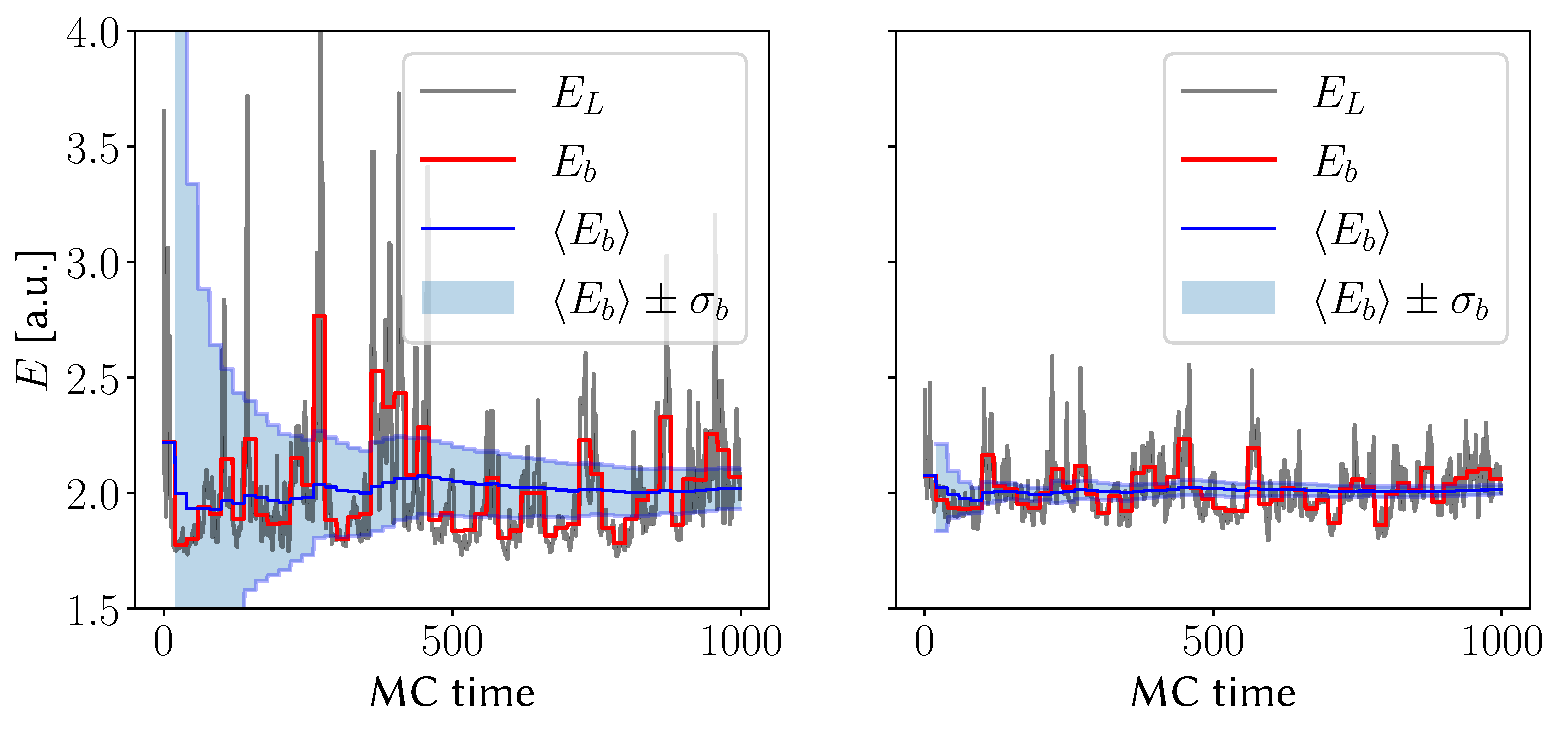
\includegraphics[width=\linewidth]{Chapter2/Figs/Vector/blocking}
	\caption[Ansatz quality in VMC]{\textbf{Ansatz quality in VMC}. Appropriateness of the variational wave function limits the quality of VMC, a poor choice of ansatz results in typical spikes in local energy  and biased result (\textbf{left}), as well as slower convergence than a good trial wave function (\textbf{right}). Figures show the local energy $E_L$, reblocked average energy $\langle E_b \rangle$ and variance $\sigma_b$ of a VMC simulation of Hookium.}
	\label{fig:qmc_blocking}
\end{figure}
VMC necessarily contains two steps, first is the estimation of the variational energy and second is the optimisation of the parameters. Any expectation of an operator $\hat{O}$ can be expressed in terms of the trial wave function as
\begin{equation}
	\langle\hat{O}\rangle=\frac{\langle\Psi_{T}\mid\hat{O}\mid \Psi_{T}\rangle}{\langle\Psi_{T} \mid \Psi_{T}\rangle}=\frac{\sum_{x}\langle\Psi_{T} \mid x\rangle\langle x\mid\hat{O}\mid \Psi_{T}\rangle}{\sum_{x}\langle\Psi_{T} \mid x\rangle\langle x \mid \Psi_{T}\rangle},
\end{equation}
where $\mid x \rangle$ are orthogonal and normal states of the Hilbert space. If we rewrite the above expression as 
\begin{equation}
	\label{eq:vmc-local_op_sampling}
	\langle \hat{O} \rangle = \frac{\sum_{x}\mid\Psi_{T}(x)\mid^{2} \hat{O}_{L}(x)}{\sum_{x}\mid\Psi_{T}(x)\mid^{2}},
\end{equation}
with $\hat{O}_L$ being the \emph{local operator}
\begin{equation}
	\hat{O}_{L}(x)=\frac{\langle x\mid\hat{O}\mid \Psi_{T}\rangle}{\langle x \mid \Psi_{T}\rangle}, 
\end{equation}
	we can interpret $|\Psi(x)|^{2}/\sum_{x}|\Psi(x)|^{2}$ as a probability. Meaning that eq.~\eqref{eq:vmc-local_op_sampling} can be estimated as an average of the local operator $\hat{O}_L$
\begin{equation}
	\langle\hat{O}\rangle \approx \frac{1}{M} \sum_{m=1}^{M} \hat{O}_{L}\left(x_{m}\right),
\end{equation}
sampled from this probability distribution. The sampling can be done using Markov Chain Monte Carlo (MCMC). The second step of the procedure is variational optimisation of the trial wave function, where the optimal parameters of the approximation are found by minimising the \emph{cost function}. The straightforward choice of the variational energy $E_V$ as a cost function turns out to be inferior to minimizing the \emph{variance} of the energy $\sigma_E$~\cite{foulkes2001quantum}. This is because $\sigma_E$ obeys the \emph{zero-variance} property, meaning that if $\Psi_{T}$ is an exact eigenvalue of the Hamiltonian
\begin{equation}
	\hat{H}\left|\Psi_{T}\right\rangle=E_{V}\left|\Psi_{T}\right\rangle,
\end{equation}
then the local energy $E_L$ is constant and equal to $E_V$
\begin{equation}
	E_{L}(x)=\Psi_{T}(x)^{-1} \hat{H} \Psi_{T}(x)=\Psi_{T}(x)^{-1} E_{V} \Psi_{T}(x)=E_{V},
\end{equation}
irrespective of the sampled configuration $x$ and hence has zero variance. The zero-variance property has important consequences for numerical stability of optimisation, it means that energy variance minima are robust to finite sampling. Minimizing the variance of energy drives the trial wave function towards eigenstates of the Hamiltonian. Moreover, the statistical error of any expectation value $\langle \hat{O} \rangle$ is proportional to the variance of $\hat{O}$, making low variance doubly desirable. There are several approaches to updating the parameters each iteration, gradient descent, stochastic reconfiguration~\cite{sorella1998green}, and the linear method~\cite{nightingale2001optimization} are just a few examples. It is crucial that the methods are robust to statistical noise and converge quickly as the MC step can be expensive to perform. Moreover they are only as good as the estimates of the energy (variance) gradients w.r.t the parameters.

The first application of VMC was to the ground state ${}^4$He~\cite{mcmillan1965ground} and it was later extended for studying many-body fermionic systems~\cite{ceperley1977monte}. Time-dependant variants of this method exist~\cite{becca2017quantum} and VMC has been used to study non-equilibrium properties of bosonic~\cite{carleo2012localization, carleo2014light}, and fermionic~\cite{ido2015time} systems.

%% Green function QMC and Diffusion QMC
\subsubsection{Projector QMC (PMC) techniques}
PMC is a class of QMC methods which are in essence nothing more than stochastic implementations of the power method to obtain the dominant eigenvector of a matrix or a kernel function~\cite{gubernatis_kawashima_werner_2016}. Their distinct advantage over VMC is that they are not constrained by our parametrisation of the trial wave function, as they can describe arbitrary probability distributions. PMC methods are based on the imaginary Schr\" odinger equation
\begin{equation}
	\label{eq:imgsch}
	\partial_{t}\left|\Psi_{t}\right\rangle=-\hat{H}\left|\Psi_{t}\right\rangle.
\end{equation}
Its formal solution, the time propagation of an initial wave function $|\Psi_0\rangle$ at $t=0$, is written as
\begin{equation}
\left| \Psi_{t} \right\rangle = e^{-\hat{H} t}\left|\Psi_{0}\right\rangle. 
\end{equation}
From the spectral decomposition of the operator $e^{-\hat{H} t}$ in terms of eigenstates $|\Phi_n\rangle$ and eigen-energies $E_n$ of the Hamiltonian $\hat{H}$
\begin{equation}
e^{-\hat{H} t}=\sum_{n} e^{-E_{n} t}|\Phi_n\rangle\langle\Phi_n|, 
\end{equation}
it follows that the term corresponding to the ground state of the system $|\Phi_0\rangle$ decays the slowest. Thus starting in some initial state and propagating for a long imaginary time $it$ leads into the ground state with the decay rate giving the ground state energy $E_0$ as
\begin{equation}
\label{eq:long_time_limit_isch}
\lim_{t \rightarrow \infty} | \Psi_t \rangle \propto e^{-E_0 t} | \Phi_0 \rangle,
\end{equation} 
where $|\Phi_0\rangle$ is the corresponding state of $E_0$. This of course holds if the eigenstates of $\hat{H}$ are all positive, which can be achieved by shifting the potential by a constant energy $E_c$, which doesn't change the ground state wave function. The basic step of a PMC simulation is the projection step, where an existing ensemble of configurations is projected into a new one, this projection $\hat{P}$ is done in such a way that eq.~\eqref{eq:long_time_limit_isch} is satisfied
\begin{equation}
	| \Phi_{0}\rangle = \lim_{n\rightarrow \infty} \hat{P}^n |\Psi_{0}\rangle.
\end{equation}
Flavours of PMC differ in the choice of $\hat{P}$, the most popular Diffusion Monte Carlo (DMC)~\cite{foulkes2001quantum, reynolds1990diffusion} works with the time-dependent Green's function $G(x^\prime, t^\prime; x, t)$ of eq.~\eqref{eq:imgsch}
\begin{equation}
	\Psi(x, t)=\int G\left(x, t; x^\prime, t^\prime\right) \Psi \left(x^{\prime}, t^\prime \right) \mathrm{d} x^{\prime},
\end{equation}
while Green's function MC (GFMC)~\cite{kalos1962monte, kalos1966stochastic} uses the time integrated version of the Green's function
\begin{equation}
	\Psi^{(n+1)}(x)=E \int G\left(x, x^{\prime}\right) \Psi^{(n)}\left(x^{\prime}\right) \mathrm{d}x^\prime. 
\end{equation}
Both formulations are exact, but need some additional approximations to be made practical for use, as Green's functions are not known for a general system. In DMC the Green's function
\begin{equation}
	G(x^\prime, t^\prime; x, t) = \langle x \mid e^{-(t-t^\prime) [\hat T + \hat V - E_c ] } \mid x^\prime \rangle,
\end{equation}
is approximated for short times $\tau = t-t^\prime$ using Trotter-Suzuki formula
\begin{equation}
	\label{eq:short_time_dmc}
	G(x^\prime \rightarrow x; \tau) = \underbrace{(2 \pi \tau)^{-3N / 2} e^{-\frac{\left(x-x^{\prime}\right)^{2}}{2 \tau}}}_{\text{ordinary diffusion}} \cdot \underbrace{e^{-\tau\left[V(\mathbf{R})+V\left(\mathbf{R}^{\prime}\right)-2 E_{c}\right] / 2}}_{\text{reweighting $\equiv$ birth/death}} + \mathcal{O}(\tau^3),
\end{equation}
where the kinetic term is recognised to be ordinary diffusion. In practice eq.~\eqref{eq:short_time_dmc} is implemented as a simulation of a diffusion process, but instead of weighting the paths of the walkers, the potential contribution to $G$ is interpreted as a probability of a walker to either branch or die, which is numerically more stable. This stochastic process converges to the ground state for sufficiently long times, see Fig.~\ref{fig:dmc}. Reptation quantum Monte Carlo~\cite{reynolds1990diffusion} (RMC) is an alternative formulation which only uses a single walker, and instead of branching and dying the MC moves mutate the path of that single walker. 
\begin{figure}[h]
	\centering
	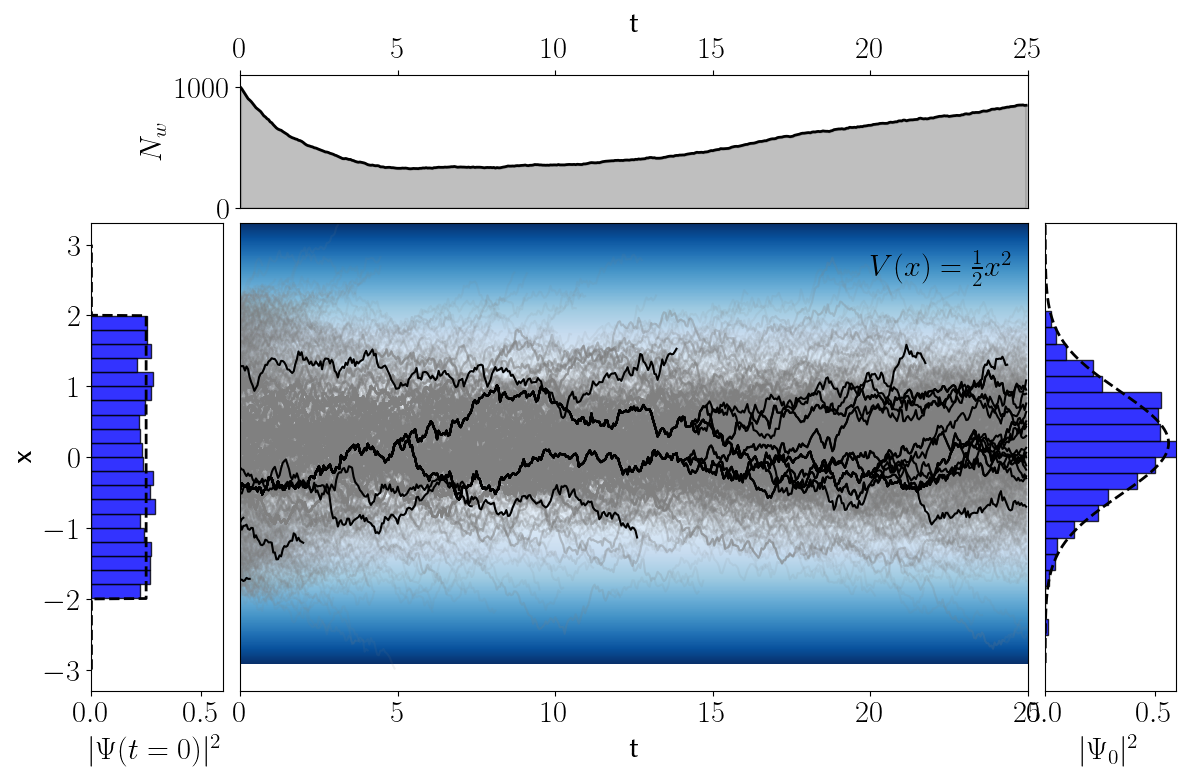
\includegraphics[width=\linewidth]{Chapter2/Figs/Raster/dmc.png}
	\caption[DMC simulation of harmonic oscillator]{\textbf{Diffusion Monte Carlo simulation of harmonic oscillator}, starting with $N_w=1000$ walkers, $\tau=0.05$, $E_c=0.25$ and uniformly sampling their initial positions from $(-2, 2)$ (\textbf{left}). The number of walkers at each step decreases rapidly before slowly increasing (\textbf{top}) the number of walkers is controlled by adjusting $E_c$. Walker paths, with a few highlighted in black to emphasise death/birth process (\textbf{middle}), diffuse into the approximate ground state of the HO $u_0(x) = \frac{1}{\pi^{\frac{1}{4}}}e^{-\frac{1}{2}x^2}$ (\textbf{right}).}
	\label{fig:dmc}
\end{figure}
Using a trial wave function $\Psi_T$ as a guiding function for importance sampling is an important improvement over vanilla DMC. This introduces a \emph{drift} into the diffusion process, which leads the walkers into regions of large values of $\Psi_T$ and greatly improves the statistical efficiency of the method. The guiding wave function is usually obtained by means of VMC. So far we have conveniently assumed that the wave function is positive everywhere in the domain, this not generally true, e.g. in fermionic systems, and poses a problem for PMC methods.

\subsubsection{The sign problem}
Projector Monte Carlo methods can only operate with positive distributions, and as such they fall apart when applied to fermionic or frustrated systems~\cite{gubernatis_kawashima_werner_2016}. A straightforward modification to the sampling scheme allows us to sample from a mixed-sign distribution. We sample from the distribution normally when it is positive, but sample from its absolute value and change the sign of the observable, when it is negative. The issue with this approach is that the population of configurations is split between positive and negative regions, the averages over both are comparable in size and cancel out, leading to a large statistical error compared to the observable. We refer to the accompanying exponential decrease~\cite{gubernatis_kawashima_werner_2016} in sampling efficiency with system size and temperature, \textbf{the sign problem}. Its general solution was shown to be NP-hard~\cite{troyer2005computational}, and as it is believed that P $\neq$ NP, this implies that no \emph{general} polynomial-time solutions exist. However, this does not mean that the problem cannot be avoided in special cases, the search for solutions is still an area of active research~\cite{hutcheon2020stochastic, assaraf2007fermion, alexandru2020complex}. In practice the sign problem is remedied by the \emph{fixed-node}~\cite{anderson1975random} or \emph{constrained-path}~\cite{zhang1997constrained} approximation. Fixed-node imposes a boundary condition into the projection such that the projected state shares the nodal surface with the trial wave function. The projected state is now only exact when the nodal surface is exact.

\subsection{Machine Learning and the quantum many-body problem}

%!TEX root = ../thesis.tex

% **************************** Define Graphics Path **************************
\ifpdf
\graphicspath{{Chapter3/Figs/Raster/}{Chapter3/Figs/PDF/}{Chapter3/Figs/}}
\else
\graphicspath{{Chapter3/Figs/Vector/}{Chapter3/Figs/}}
\fi

%*******************************************************************************
%****************************** Third Chapter **********************************
%*******************************************************************************

\newtheorem{theorem}{Theorem}[section]
\newtheorem{corollary}{Corollary}[theorem]
\newtheorem{lemma}[theorem]{Lemma}
\newtheorem{definition}{Definition}[section]

\chapter{Feynman-Kac: connecting Quantum Mechanics and Stochastic Processes}
\label{chapter3}
In this chapter we will provide a bridge between the quantum many-body problem discussed in the previous chapter and stochastic processes. This will entail introducing the Feynman-Kac formula and relating it to the Fokker-Planck equation and optimal control formulations of QM. Moreover, a probabilistic view of the cost function will lead us to proposals for loss functions that can be used to learn optimal transition rates and consequently sample the ground state.

The field of stochastic processes is a vast body of work, approached from different angles by mathematicians, physicists and engineers. A necessary consequence of this is that the literature ranges from extremely thorough and rigorous~\cite{rogers1994diffusions, rogers2000diffusions} to more applied and intuitive~\cite{sarkka2019applied}. For this reason, the mentioned discussion will be preceded by an overview of the mathematical notation, lemmas and results from stochastic processes and measure theory that underpin some core ideas of this thesis. To avoid including a whole textbook of material on measure and stochastic processes some concepts will not be rigorously defined, the text will point to relevant literature where this is the case.

\section{Stochastic processes}
\label{subsec:fk-stoch}
\subsection{Fundamentals}
This brief, more formal, discussion of stochastic processes is based mostly upon classic texts~\cite{durrett2019probability, rogers1994diffusions, rogers2000diffusions} and borrows some intuitions from~\cite{sarkka2019applied}. The most basic quantity that we will need is the \textbf{probability space}. 
\begin{definition}[Probability space]
	The probability space is a tuple $(\Omega, \mathcal{F}, \mathbb{P})$, where $\Omega$ is the \textbf{sample space}, $\mathcal{F}$ is a $\sigma$-\textbf{field}, and $\mathbb{P}$ is the \textbf{measure}.
\end{definition}
The sample space is simply the set of all possible outcomes. A canonical example would be the roll of a 6-sided dice, $\Omega=\{1, 2, 3, 4, 5, 6\}$. Without measure $\mathbb{P}$, the tuple $(\Omega, \mathcal{F})$ is termed a \textbf{measurable space}.
\begin{definition}[$\sigma$-field]
	A $\sigma$-field $\mathcal{F}$ on a set $\Omega$, is a nonempty collection of subsets of $\Omega$ that includes $\Omega$ itself, is closed under complement, i.e. if $A \in \mathcal{F}$ then $A^c \in \mathcal{F}$, and is closed under countable unions, $\cup_{i} A_{i} \in \mathcal{F}$ if $A_{i} \in \mathcal{F}$ is a countable union of sets.
\end{definition}
The main utility of the $\sigma$-field to us is its use in defining measures. We want to be able to assign a non-negative real number to all subsets of $\Omega$, as well as the size of the union of the disjoint sets to be the sum of their individual sizes. This is not always possible, a counterexample for the real line being Vitali sets. The collection $\mathcal{F}$, must thus only include \emph{measurable} sets, which are precisely the ones that satisfy the constraints imposed by the $\sigma$-field.
\begin{definition}[Measure]
	A non-negative countably additive set function $\mu: \mathcal{F} \rightarrow \mathbb{R}$ that satisfies
	\begin{enumerate}[label=\roman*)]
		\item $\mu(A) \geq \mu(\emptyset)=0$ for all $A \in \mathcal{F}$
		\item if $A_{i} \in \mathcal{F}$ is a countable sequence of disjoint sets, then $\mu\left(\cup_{i} A_{i}\right)=\sum_{i} \mu\left(A_{i}\right)$
	\end{enumerate}
	is a \textbf{measure}.
\end{definition}
If $\mu(\Omega)=1$, then $\mu$ is a \textbf{probability measure} and will be denoted by $\mathbb{P}$. With this notion we are now able to define a random variable (r.v) and a stochastic process (s.p.).
\begin{definition}[Random variable]
	 A \textbf{random variable} $X$ defined on $\Omega$ is a real-valued measurable function $X(\omega)$, $X: \Omega \rightarrow \mathbb{R}^d$.
\end{definition}
For a function to be measurable, we require that its preimage $X^{-1}$ is in the $\sigma$-field $\mathcal{F}$
\begin{equation}
	X^{-1}(B) = \{ \omega : X(\omega) \in B \} \in \mathcal{F},
\end{equation}
and that this holds for every Borel set $B$ in the Borel $\sigma$-field~\footnote{For a proper definition of the Borell set see ch. 3 of~\cite{salamon2016measure}.} of $\mathbb{R}^d$, which is simply the smallest $\sigma$-field that contains all measurable sets in $\mathbb{R}^d$. 

A random variable $X$ induces a probability measure $\mu$ on $\mathbb{R}^d$ called its \textbf{distribution}, this is done by setting $\mu(A)=P(X \in A)$ for Borel sets $A$. Moreover, the distribution is usually given in terms of a \textbf{distribution function} $F(x)$
\begin{equation}
	 F(x) = \mathbb{P}(\{\omega \in \Omega: X(\omega) \leq x\}) = \mathbb{P}(X \leq x),
\end{equation}
and $X$ is said to have a \textbf{density function} $f(x)$ if $F(x)$ can be written as 
\begin{equation}
	\label{eq:pdf}
	F(x)=\int_{-\infty}^{x} f(y) \mathrm{d}y.
\end{equation}
In essence, the random variable provides a connection between the less familiar probability measure $\mathbb{P}$ and the cumulative distribution function (CDF).

\subsection{Stochastic process}
\begin{definition}[Stochastic process]
		Given a probability space $(\Omega, \mathcal{F}, \mathbb{P})$ and a measurable (state) space $(E, \mathcal{E})$, we define the collection $\left\{X_{t}: t \in T\right\}$ of set $T$ indexed and $(E, \mathcal{E})$ valued random variables a \textbf{stochastic process}.
\end{definition}
By far the most common case for the index set $T$, is time $T = \mathbb{R}^+$. Such s.p's are called \emph{temporal}, examples include the model of velocity of a Brownian particle under influence of friction, in Fig.~\ref{fig:sp-brown}, or the Black-Scholes model. Nevertheless, the index set is not limited to time, as is often the case with Gaussian Process regression~\cite{rasmussen2006gaussian}. In this thesis we will mostly deal with temporal s.p's of the kind that do not "see into the future". This notion is formalized using \textbf{filtrations}. A filtration $\mathbb{F}=\left(\mathcal{F}_{t}\right)_{t \in T}$ on a probability space $(\Omega, \mathcal{F}, \mathbb{P})$ is just an increasing sequence or order of $\sigma$-fields
\begin{equation}
	\mathcal{F}_{s} \subset \mathcal{F}_{t} \text { if } 0 \leq s \leq t<\infty
\end{equation}
The filtration associated to a process that records its "past behaviour" at each time is called the \textbf{natural filtration}. 
\begin{definition}[Adapted process]
	A process $\{X_t\}$ is said to be \textbf{adapted to the filtration} $\left(\mathcal{F}_{t}\right)_{t \in T}$ if the random variable $X_t : \Omega \rightarrow E$ is $\mathcal{F}_t$-measurable function for each $t \in T$. 
\end{definition}
A process that is \emph{non-anticipating}, i.e. depends only on the past and present, is adapted to the filtration $\left(\mathcal{F}_{t}\right)_{t \in T}$.
\begin{definition}[Brownian motion]
	\textbf{Brownian motion} or a non-anticipating \textbf{Wiener process} is a stochastic process $W_t$, with the following properties:
	\begin{enumerate}[label=\roman*)]
		\item $W_0 = 0$
		\item $W_t$ is almost surely continuous in t
		\item $W_t$ has independent increments
		\item $W_t - W_s \sim \mathcal{N} (0, t-s)$ for $0 \leq s \leq t$
	\end{enumerate}
\end{definition}
\noindent
A realisation of Brownian motion can be found in Fig.~\ref{fig:sp-brown}.
\begin{figure}[h]
	\centering
	\subfloat{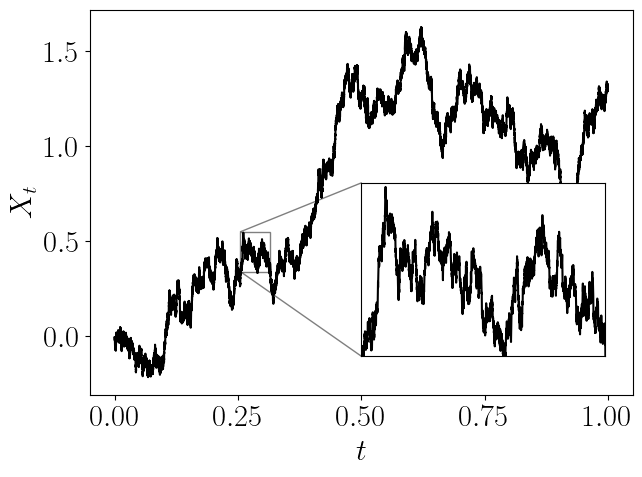
\includegraphics[width=0.5\linewidth]{Chapter3/Figs/Raster/OU-BM-I.png}}
	\subfloat{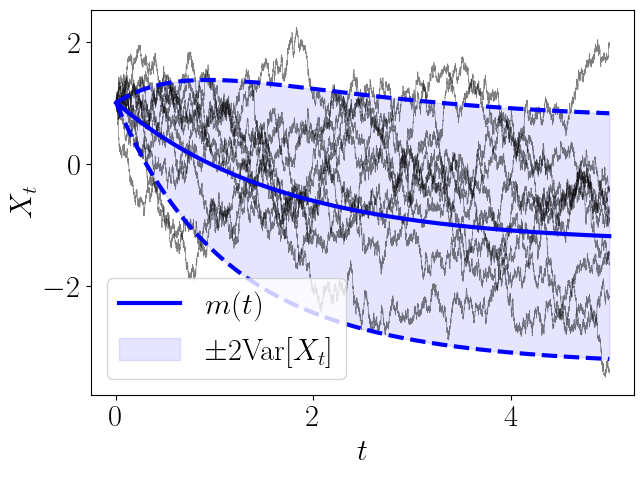
\includegraphics[width=0.5\linewidth]{Chapter3/Figs/Raster/OU-BM-II.png}}
	\caption[Brownian motion and Ornstein–Uhlenbeck process
	]{\textbf{Brownian motion and Ornstein–Uhlenbeck process.} 
		\textbf{left:} A single realisation of the Brownian process. \textbf{right:} Mean, variance and 10 samples of the Ohrnstein-Uhlenbeck process with $\theta=0.6, \sigma=1.1, X_0=1.0, \mu=-1.3$, integrated using Euler-Maruyama method.}
	\label{fig:sp-brown}
\end{figure}

\subsection{Integrals}
In order to proceed and define stochastic differential equations (SDE's) and the Radon-Nikodyn derivative, we must spend some time discussing various integrals we will use. In particular, alongside the usual Riemann integral, we will need three more types of integrals, which we will briefly describe without mathematical derivation. The simplest kind of integral we will introduce is the integral of a stochastic process
\begin{equation}
	I = \int_{0}^{t} X_t \mathrm{d}t.
\end{equation}
The simple appearance of the integral is deceiving as the integrand is a realisation of a $\mathcal{F}_t$-adapted stochastic process $\{X_t\}: \Omega \times T \rightarrow \mathbb{R}^{d}$, meaning that $I$ itself is a random variable. However, since each realisation of $X_t$ is almost surely continuous, $I$ can be expanded as a Riemann sum, which converges under mean-squared norm to $I$, so long as the mean $\mathbf{m}(t) = \mathbb{E}[X_t]$ and covariance $\textbf{k}(t,s) = \operatorname{Cov}(X_t, X_s)$ are continuous. In practice, computing the mean and covariance of $I$ is usually enough to understand the resulting stochastic process. Importantly, integrals of continuous functions of s.p's $h(X_t),~ h: \mathbb{R} \rightarrow \mathbb{R}$ can be computed in a similar manner.

The second type of integrals we need to consider, are integrals with respect to a s.p, known as \textbf{It\^ o integrals}
\begin{equation}
	\label{eq:ito}
	Y_t = \int_{0}^{t} H_s \mathrm{d}X_s,
\end{equation}
where both $H_s$ and $X_s$ are stochastic processes. The result integral $Y_t$ is itself a stochastic process which resides in the probability space $(\Omega, \mathcal{F}, \mathbb{P})$, filtered by $\left(\mathcal{F}_t\right)_{t\in T}$. The integral can be formalised by putting slight constraints on what sort of stochastic processes $X_s$ and $H_t$ can be, expanding $Y_t$ as a Riemann sum and proving convergence. Details of this procedure can be found in~\cite{rogers2000diffusions}.

Finally we must define the \textbf{Lebesgue-Stieltjes integral}~\cite{halmos2013measure}, which we need to properly define expectations of stochastic processes. 
\begin{definition}[Lebesgue-Stieltjes Integral]
		Given probability space $(\Omega, \mathcal{F}, \mathbb{P})$ and measurable function $f:\Omega \rightarrow \mathbb{R}$, the \textbf{Lebesgue-Stieltjes integral} 
		\begin{equation}
			I = \int_A f(x) \mathrm{d}\mathbb{P}(x),
		\end{equation}
		is the Lebesgue integral~\footnote{For proper definition of the Lebesgue integral see ch. 1 of~\cite{salamon2016measure}.} with respect to measure $\mathbb{P}$, $A \in \mathcal{F}$.
\end{definition}
With it we can define expectations in the probability space $(\Omega, \mathcal{F}, \mathbb{P})$ as
\begin{equation}
	\underset{{\mathbb{P}}}{\mathbb{E}}[f(x)]=\int_{\Omega} f(x) d \mathbb{P}(\boldsymbol{x}).
\end{equation}
For a newcomer to stochastic processes this formulation may seem redundant, can we not just calculate expectations using a Riemann integral and the PDF? We can, and when the distribution $\mathbb{P}$ can be expressed in terms of the PDF~\eqref{eq:pdf}, the Lebesgue integral can be interpreted in this way. However, stochastic processes need not admit a PDF, that is when the Lebesgue-Stieltjes integral is necessary.
%\begin{equation}
%	\int_{\Omega} f(x) \mathrm{d} \mathbb{P}(x)=\int_{\Omega} f(x) p(x) d \lambda(x)
%\end{equation}
\subsection{Stochastic Differential Equations}
In this thesis we will refer to a SDE as an informal notation of an It\^ o integral equation or \textbf{It\^ o process}. 
\begin{definition}[It\^ o process]
	Given deterministic functions $v: \mathbb{R}^{d} \times \mathbb{R}^{+} \rightarrow \mathbb{R}^{d}$ and $\sigma: \mathbb{R}^{d} \times \mathbb{R}^{+} \rightarrow \mathbb{R}^{d \times d}$, we define the \textbf{It\^ o process} $X_t$ as the sum of It\^ o and Lebesgue integrals
	\begin{equation}
		\label{eq:ito-process}
		X_{t+s}-X_{t}=\int_{t}^{t+s} \sigma\left(X_{u}, u\right) \mathrm{d} W_{u} + \int_{t}^{t+s} v\left(X_{u}, u\right) \mathrm{d} u,
	\end{equation}
	where $W_t$ is a Brownian motion.
\end{definition}
In simplified notation we can write~\eqref{eq:ito-process} as
\begin{equation}
	\label{eq:SDE_general}
	\mathrm{d} X_t = \sigma \left(X_{t}, t\right)\mathrm{d}W_t + v\left(X_{t}, t\right) \mathrm{d}t,
\end{equation}
this is what we refer to as an SDE, an example can be found in Fig.~\ref{fig:sp-brown}. The functions $v$ and $\sigma$, we will refer to as the \textbf{drift} and \textbf{volatility} of the It\^ o process respectively. The most intuitive interpretation of a SDE is in terms of the time evolution of the PDF of the process $X_t$. It is described by the \textbf{Fokker-Planck equation}~\footnote{Derivation in~\cite{sarkka2019applied}.} 
\begin{equation}
	\label{eq:Fokker-Planck-General}
	\frac{\partial p(\mathbf{x}, t)}{\partial t}=
	-\sum_{i=1}^{N} \frac{\partial}{\partial x_{i}}\left[\mu_{i}(\mathbf{x}, t) p(\mathbf{x}, t)\right]
	+\sum_{i=1}^{N} \sum_{j=1}^{N} \frac{\partial^{2}}{\partial x_{i} \partial x_{j}}\left[D_{i j}(\mathbf{x}, t) p(\mathbf{x}, t)\right],
\end{equation}
where $p(\mathbb{x}, t)$ is the PDF of the solution to the SDE and $\mathbf{D}=\frac{1}{2} \boldsymbol{\sigma} \boldsymbol{\sigma}^{\top}$ is the diffusion tensor. Finally we state without proof a consequence of It\^ o calculus, most commonly named \textbf{It\^ o's rule} or \textbf{lemma}, it is the stochastic calculus equivalent of the chain rule
\begin{lemma}[It\^ o's lemma]
	Given an It\^ o process $X_t$ as given by ~\eqref{eq:ito-process} and a twice differentiable scalar function $f(X_t, t)$, then the It\^ o process for $f$ is
	\begin{equation}
		\label{eq:ito_lemma}
		\mathrm{d} f = \frac{\partial f}{\partial t}\mathrm{d}t + \sum_i \frac{\partial f}{\partial x_i} \mathrm{d}x_i + \frac{1}{2}\sum_{ij} \frac{\partial^{2}}{\partial x_{i} \partial x_{j}} f \mathrm{d}x_i \mathrm{d}x_j,
	\end{equation}
\end{lemma}
when compared to ordinary calculus we notice an additional quadratic term.

\subsection{Radon-Nikodym Derivative and Girsanov theorem}
To perform importance sampling we perform a change of measure in an integral
\begin{equation}
	\int_{A} f(x) \mathrm{d} \mathbb{P}(x)=\int_{A} f(x) \frac{\mathrm{d} \mathbb{P}}{\mathrm{d} \mathbb{Q}}(x) \mathrm{d} \mathbb{Q}(x).
\end{equation}
The function that measures the rate of change of density of one measure w.r.t another is the \textbf{Radon-Nikodym derivative} $\frac{\mathrm{d} \mathbb{P}}{\mathrm{d} \mathbb{Q}}(x)$.

\begin{theorem}[Radon-Nikodym theorem]
	Let $\mathbb{P}$ and $\mathbb{Q}$ be probability measures on the measurable space $(\Omega, \mathcal{F})$, then the measurable function \textbf{Radon-Nikodym derivative} $\frac{\mathrm{d} \mathbb{P}}{\mathrm{d} \mathbb{Q}}(x): \Omega \rightarrow[0, \infty)$ exists and 
	\begin{equation}
		\mathbb{P}(A)=\int_{A} \frac{\mathrm{d} \mathbb{P}}{\mathrm{d} \mathbb{Q}}(x) \mathrm{d} \mathbb{Q}(x),
	\end{equation}
	for set $A \subseteq \mathcal{F}$.
\end{theorem}
The RN derivative will also be useful in defining the KL divergence between two \textbf{path measures}. Properly defining the path measure would bring a lot of notational overhead, it is enough to think of it as a measure on the \textbf{path space}, i.e all possible paths of a SDE, for rigour see~\cite{leonard2014pathmeasure}. 
Finally, we state the \textbf{Girsanov theorem} that is often used for transforming or removing drift functions of SDE, it is the RN derivative between an It\^ o process and one with $v = 0$ and $\sigma = 1$, i.e. Brownian motion. 
\begin{theorem}[Girsanov Theorem]
	Given It\^ o process
	\begin{equation}
		\mathrm{d}X_t = \mathrm{d}W_t + v(X_t, t)\mathrm{d}t \quad \text{and} \quad X_0 = 0 \\
	\end{equation}
	and Brownian motion $\mathrm{d}Y_t = \mathrm{d}W_t$, the RN derivative of their respective path measures $\mathbb{P}$ and $\mathbb{P}_0$	is
	\begin{equation}
		\label{eq:Girsanov_theorem}
		\frac{\mathrm{d} \mathbb{P}}{\mathrm{d} \mathbb{P}_0}=
		\exp \left(
		-\frac{1}{2} \int_{0}^{t}\left|v(X_s, s)\right|^{2} \mathrm{d} s+\int_{0}^{t} v(X_s, s)^{\top} \mathrm{d} W_s\right)
	\end{equation}
\end{theorem}

\noindent
This \emph{change in dynamics} as we will call it later is true in the sense, that expectations for an arbitrary functional $h(\cdot)$ of the path from $0$ to $t$ are
\begin{equation}
	\label{eq:girsanov_consequence}
	\underset{\mathbb{P}}{\mathbb{E}}\left[h(X_t)\right] = \underset{\mathbb{P}_0}{\mathbb{E}}\left[\frac{\mathrm{d} \mathbb{P}}{\mathrm{d} \mathbb{P}_0} h(Y_t)\right]. 
\end{equation}
For a more general case and proof see~\cite{sarkka2019applied}.

\subsection{Markov processes}
We now shift our view to a special kind of s.p's, ones that satisfy the \textbf{Markov property} called \textbf{Markov processes} or \textbf{Markovian}. The property is sometimes referred to as \emph{memorylessness}, as the future of a Markov process depends only on the present state. We can classify the processes based on the system's \textbf{state-space} $S$, which can be either discrete (countable) or continuous, and the \textbf{time indexing} of the system, either discrete-time $\{X_n\}_{n \geq 0}$ or continuous-time $\{X_t\}_{t \geq 0}$. A taxonomy is given in Table~\ref{tab:MP-taxonomy}. We will not specifically discuss Markov processes in continuous state-space, but it is important to note that any It\^ o process with time-homogenous drift $v = v(X_t)$ and volatility $\sigma = \sigma(X_t)$ is Markovian.

From now on we refer to Markov processes in countable state-space as \textbf{Markov chains}. We base our discussion on~\cite{rogers1994diffusions} and~\cite{norris1998markov}. 
\begin{table}[h]
	\begin{center}
		\caption[Taxonomy of Markov processes]{\textbf{Taxonomy of Markov processes}}
		\label{tab:MP-taxonomy}
		\begin{tabular}{p{2cm}|p{6cm}|p{6cm}}
%			\toprule % <-- Toprule here
			 & Countable state-space & Continuous state-space\\
			\midrule
			Discrete time 
			&\parbox{5cm}{\textbf{index: }$\{X_n\}_{n \geq 0}$, $n \in \mathbb{Z}^{+}$ \\ \textbf{state-space: } countable set $I$ \\ \textbf{define: } stochastic $\{P\}_{ij}$ \\ \textbf{example:} DTMC}  
			&\parbox{5cm}{\textbf{index: }$\{X_n\}_{n \geq 0}$, $n \in \mathbb{Z}^{+}$ \\ \textbf{state-space: } general state-space $\Omega$ \\ \textbf{define: } stochastic kernel $K$ \\ \textbf{example:} Harris Chain}\\
			\midrule
			Continuous time 
			&\parbox{5cm}{\textbf{index: }$\{X_t\}_{t \geq 0}$, $t \in \mathbb{R}^{+}=[0, \infty)$ \\ \textbf{state-space: } countable set $I$ \\ \textbf{define: } rate $\{\Gamma\}_{ij}$ equiv. to jump chain $\{J_n\}_{n\geq0}$ and hold times $\{S_n\}_{n\geq1}$. \\ \textbf{example:} CTMC}
			&\parbox{5cm}{\textbf{index: }$\{X_t\}_{t \geq 0}$, $t \in \mathbb{R}^{+}=[0, \infty)$ \\ \textbf{state-space} general state-space $\Omega$ \\ \textbf{define: } stochastic kernel $K$ \\ \textbf{example:} Diffuson process}\\
			\bottomrule % <-- Bottomrule here
		\end{tabular}
	\end{center}
\end{table}
\subsubsection{Discrete-time Markov Chains}
The simplest and most common Markov process is a Markov chain in discrete time, an example of it can be found in Fig.~\ref{fig:mc-diagrams}. Its state-space is a countable set $I$ and we call each $i \in I$ a \textbf{state}. We define a distribution $\lambda$ in a familiar way
\begin{equation}
	\lambda = \{\lambda_i : i \in I\} \quad \text{where} \quad \forall i:~ 0 \leq \lambda_i < \infty \quad \text{and} \quad \sum_{i \in I} \lambda_i = 1.
\end{equation}
We can now set $\lambda$ as a distribution of some random variable $X:\Omega \rightarrow I$ as
\begin{equation}
	\lambda_{i}=\mathbb{P}(X=i)=\mathbb{P}(\{\omega: X(\omega)=i\}),
\end{equation}
where we are still working in the probability space $(\Omega, \mathcal{F}, \mathbb{P})$. A discrete-time Markov chain is defined in terms of its \textbf{transition matrix} $P=\{p_{i j}: i, j \in I\}$, which is a \textbf{stochastic matrix} meaning all of its rows $\{p_{i j}: j \in I\}$ are distributions.
\begin{definition}[Discrete-time Markov chain]
	A discrete time stochastic process $\{X_n\}_{n \geq 0}$ is a \textbf{discrete-time Markov chain} with initial distribution $\lambda$ and transition matrix $P$ if for $i_1, \dots, i_n+1 \in I$ and $n \geq 0$
	\begin{enumerate}[label=\roman*)]
		\item $\mathbb{P}\left(X_{0}=i_{1}\right)=\lambda_{i_{1}}$
		\item $\mathbb{P}\left(X_{n+1}=i_{n+1} \mid X_{0}=i_{0}, \dots, X_{n}=i_{n}\right)=p_{i_{n} i_{n+1}}$
	\end{enumerate}
\end{definition}
Rewriting the second condition above, it is clear that the Markov chain is without memory
\begin{equation}
	\mathbb{P}\left(X_{n+1}=i_{n+1} \mid X_{0}=i_{1}, \dots, X_{n}=i_{n}\right)=\mathbb{P}(X_{n+1} = i_{n+1} \mid X_{n} = i_{n}).
\end{equation}
Intuitively we understand the discrete-time Markov chain as a system changing its state at discrete time intervals, each time choosing the next state according to the row of the Transition matrix corresponding to the current state.
\begin{figure}[h]
	\centering
	\subfloat{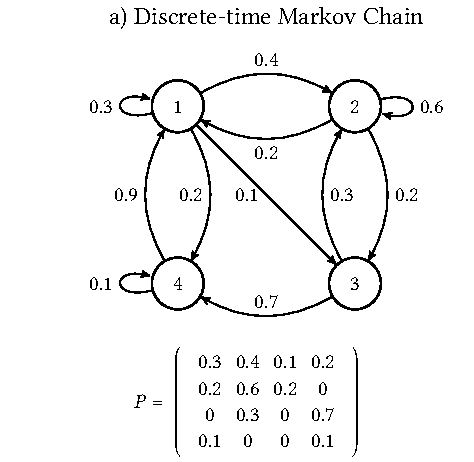
\includegraphics[width=0.5\linewidth]{Diagrams/mc_I/mc_I.pdf}}
	\subfloat{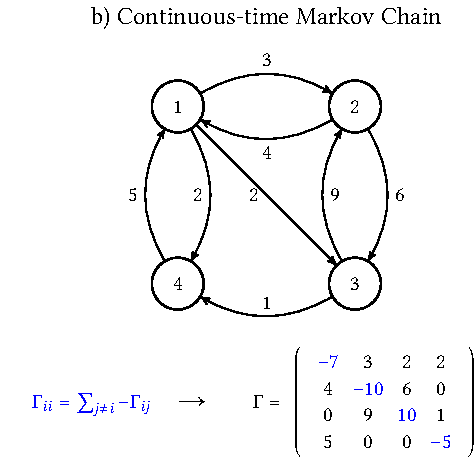
\includegraphics[width=0.5\linewidth]{Diagrams/mc_II/mc_II.pdf}}
	\caption[Discrete and continuous time Markov Chains.]{\textbf{Discrete and continuous time Markov Chains.} \textbf{left:} Discrete-time Markov Chain defined by $P$. \textbf{right:} Continuous-time Markov Chain defined by $\Gamma$.}
	\label{fig:mc-diagrams}
\end{figure}

\subsubsection{Continuous-time Markov Chains}
\label{subsubsect:CTMC}
Defining a Markov chain in continuous time is slightly trickier as describing the system with a stochastic matrix does no longer suffice because transition probabilities become zero when considering an infinitesimal time. Instead a continuous-time Markov Chain (CTMC) is characterised by a \textbf{rate matrix} or \textbf{infinitesimal generator matrix} $\Gamma$ defined on the set $I$. A rate matrix has the following three properties
\begin{enumerate}[label=\roman*)]
	\item $0 \leq \Gamma_{ii} <\infty, \quad \forall i$
	\item $\Gamma_{ij} \geq 0, \quad \forall i \neq j$
	\item $\sum_{j \in I} \Gamma_{i j}=0, \quad \forall i$
\end{enumerate}
While the CTMC can be interpreted in a number of ways, we shall use the so called \textbf{jump chain} and \textbf{holding times} representation, see also Fig.~\ref{fig:holdingJumping}. 
\begin{figure}[h]
	\centering
	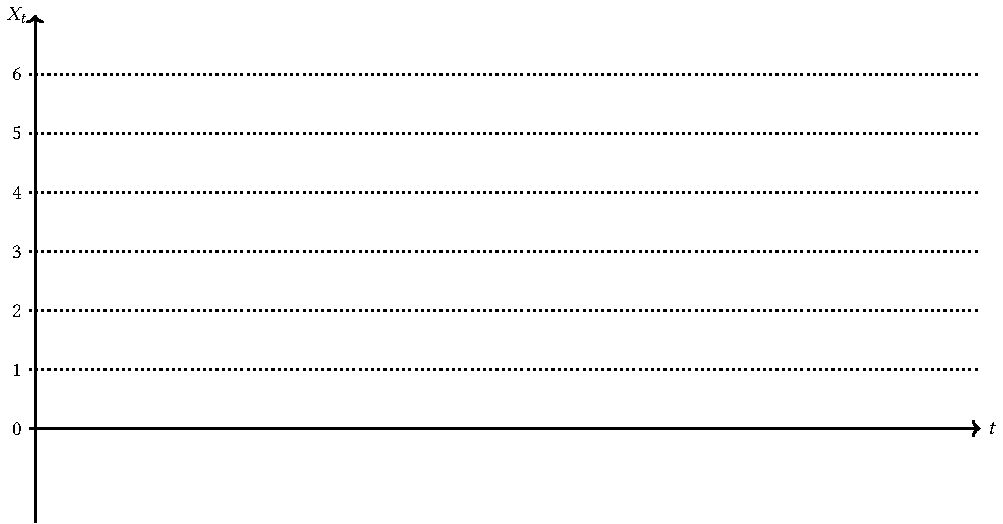
\includegraphics[width=0.9\linewidth]{Diagrams/ctmc/ctmc}
	\caption[Jump chain and Holding times]{\textbf{Jump chain and Holding times.} A discrete space Markov process $\{X_t\}_{t\geq 0}$ in continuous time. The holding times $S_n$ are independent exponential random variables and the transition probabilities at jump times $J_n$ are given with the jump matrix $\Pi$. Inspired by~\cite{norris1998markov}.}
	\label{fig:holdingJumping}
\end{figure}
We can think of a CTMC as a series of discrete jumps, where the system remains in each state for a certain holding time. This suggests that we can construct the CTMC from a discrete-time chain with stochastic matrix $\Pi$, which we will call the \textbf{jump matrix}, and a set of independent random variables $\{S_n\}$ which determine the holding times. We construct matrix $\Pi$ by rescaling rows of $\Gamma$ so they add up to one, putting a $0$ on the diagonal
\begin{equation}
	\begin{array}{l}
		\Pi_{i j}=\left\{
		\begin{array}{ll}
			\Gamma_{i j} / \Gamma_{ii} & \text { if } j \neq i \text { and } \Gamma_{ii} \neq 0 \\
			 0 & \text { if } j \neq i \text { and } \Gamma_{ii}=0
		\end{array}\right. 
		\\ 
		\Pi_{i i}=\left\{
		\begin{array}{ll}
			0 & \qquad  \text { if } \Gamma_{ii} \neq 0 \\
			1 & \qquad \text { if } \Gamma_{ii}=0.
		\end{array}\right.
	\end{array}
\end{equation}
In order for the process to possess the Markov property, the distribution of holding times $\{S_n\}$ must be exponential~\cite{norris1998markov}, 
\begin{equation}
	S_{n+1} \sim \operatorname{Exp}(-{\Gamma_{ii}}(X_n)),
\end{equation}
with exponential parameters being $-\Gamma_{ii}$ where $i$ is the current state.
Processes with different holding time distributions are called \textbf{semi-Markov}. The jump times $\{J_n\}$ are simply 
\begin{equation}
	J_{n}=S_{1}+\ldots+S_{n}.
\end{equation}
\begin{definition}[Continuous-time Markov chain]
	A stochastic process $\{X_t\}_{t \geq 0}$ on set $I$ is a \textbf{continuous-time Markov chain} if its jump chain $\{Y_n\}_{n \geq 0}$ is a discrete-time Markov chain and its holding times $\{S_n\}_{n \geq 1}$ are independent exponential random variables $S_n \sim \operatorname{Exp}(-{\Gamma_{ii}}(X_n))$.
\end{definition}
An equivalent formulation is in terms of \textbf{competing exponentials}. Transitions $\Gamma_{j \rightarrow k}$ from $j$ to $k$ are defined as independent exponential random variables $\tau_{j \rightarrow k}$
\begin{equation}
	\tau_{j \rightarrow k} \sim \operatorname{Exp}(\Gamma_{jk}), \quad j \neq k
\end{equation}
the next state is then chosen as
\begin{equation}
	Y_{n+1} = \operatorname{argmin}_{k} \tau_{j \rightarrow k}.
\end{equation}
The chain $\{Y_n\}_{n\geq0}$ along with times 
\begin{equation}
	S_{n} = \min _{k} \tau_{j \rightarrow k},
\end{equation}
gives the full description of the CTMC. With this formulation in mind we now interpret $\Gamma_{ii}$ as the rate ob \emph{leaving} current state and $\Gamma_{i j}$ as the rate of \emph{going} from $i$ to $j$.

\newpage
\section{The Feynman-Kac formula}
\label{subsec:fk-fk}
The Feynman path integral formulation introduced in chapter~\ref{chapter2} was extensively used by physicists for decades, even in the absence of a formal mathematical formulation which is hard to define because of the difficulties with defining an appropriate measure on the path space. Kac~\cite{kac1949distributions} provided a rigorous formulation of the \textit{real-valued} case of the Feynman path integral, and the resulting \textbf{Feynman-Kac formula} eq.~\eqref{eq:fkac} provides a bridge between \emph{parabolic} partial differential equations and stochastic processes. 

\subsection{Feynman-Kac in continuous state space}
\label{subsec:FK_in_continuous_space}
To illustrate the Feynman-Kac formula let us consider a single particle with Hamiltonian
\begin{equation}
	\hat{H} = -\frac{\mathrm{d}^2~~}{\mathrm{d}x^2} + V(x)
\end{equation}
and the Schr\" odinger equation in \textit{imaginary time}, which is of the parabolic type, 
\begin{equation}
	\label{eq:imag_sch}
	\partial_t | \psi_t \rangle = - \hat{H} | \psi_t \rangle.
\end{equation}
In close analogy to arguments presented in the DMC section~\ref{subsubsec-PMC}, Kac noticed that the kinetic term of the Lagrangian in eq.~\eqref{eq:FPI} could be interpreted as a measure on Brownian walks, and a solution to the imaginary time Schr\" odinger equation can be written as
\begin{equation}
	\label{eq:fkac}
	\psi(x, t)=\underset{X \sim \text { Brownian with } X_{t}=x}{\mathbb{E}}
	\left[\exp \left(-\int_{0}^{t}  V\left(X_{\tau}, \tau \right) \mathrm{d}\tau \right) \psi\left(X_{0}, 0\right)\right],
\end{equation}
where only the \textbf{endpoint} at time $t$ of the Brownian process fixed, whereas the starting point at time $t=0$ is not. $\psi (x, 0)$ encodes the initial condition into this representation. When there is no external potential $V(x) = 0$, the Schr\" odinger equation in imaginary time is the diffusion equation and the Feynman-Kac solution is simply
\begin{equation}
	\begin{aligned} 
		\psi(x, t) &= \underset{X \sim \text { Brownian with } X_{t}=x}{\mathbb{E}}\left[\psi\left(X_{0}, 0\right)\right] \\
		&=  
		\frac{1}{\sqrt{2 \pi t}} \int  e^{-\left(x-x^{\prime}\right)^{2} / 2 t} \psi_{0}\left(x^{\prime}\right) \mathrm{d} x^{\prime}
	\end{aligned}
\end{equation}
An illustration of the Feynman-Kac approach to the problem with no external potential $V(x)$ in 1D is depicted in Fig.~\ref{fig:fk_1d_example}. 
\begin{figure}[H]
	\centering
	\subfloat
	{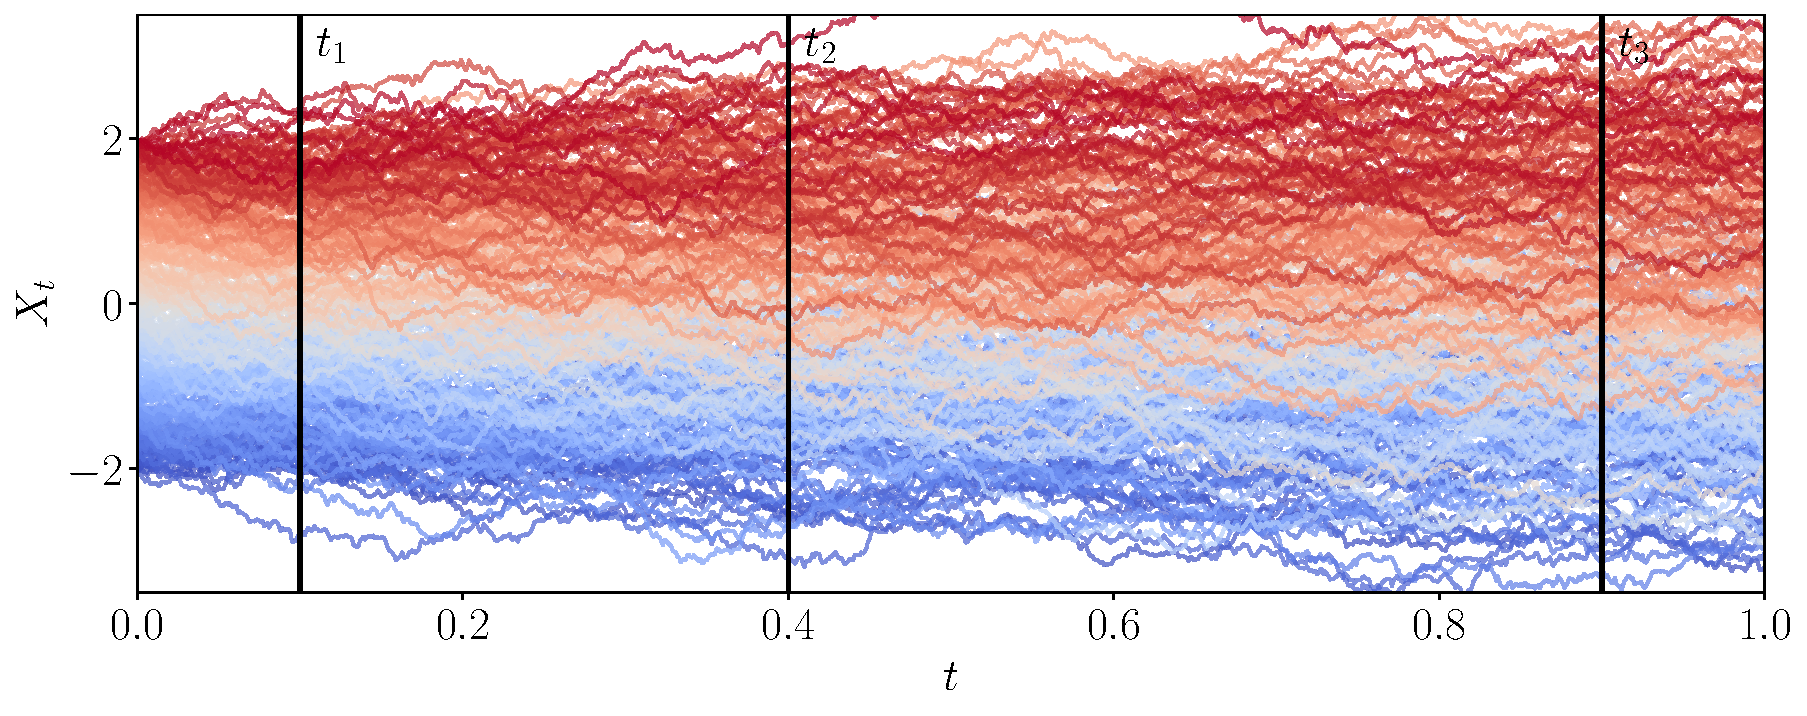
\includegraphics[width = \linewidth]{Chapter3/Figs/Raster/fkac_vs_fplanck_top.pdf}} \\
	\subfloat
	{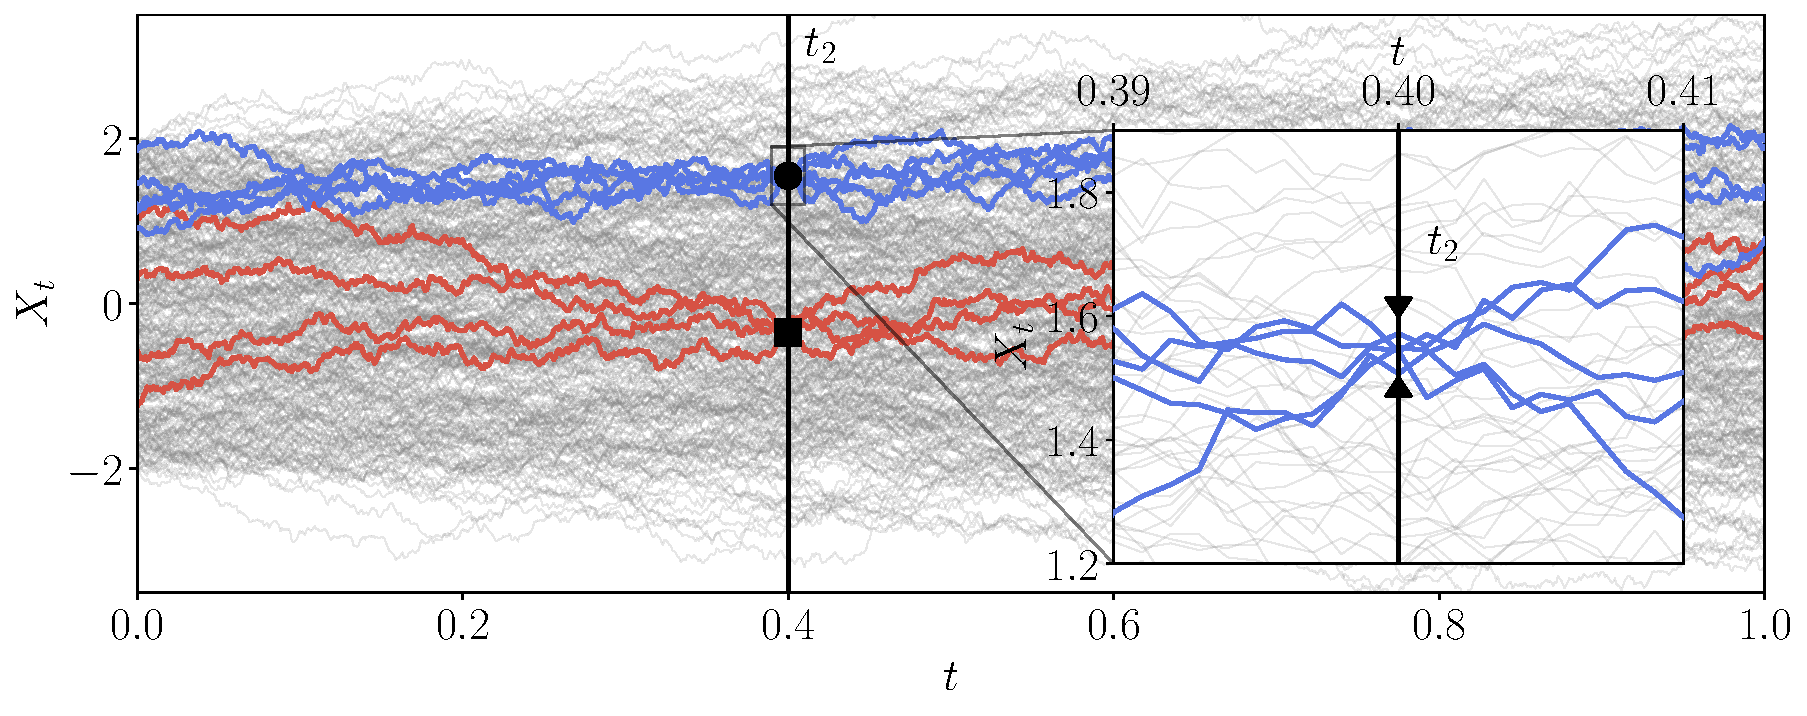
\includegraphics[width = \linewidth]{Chapter3/Figs/Raster/fkac_vs_fplanck_mid1.pdf}} \\
	\subfloat
	{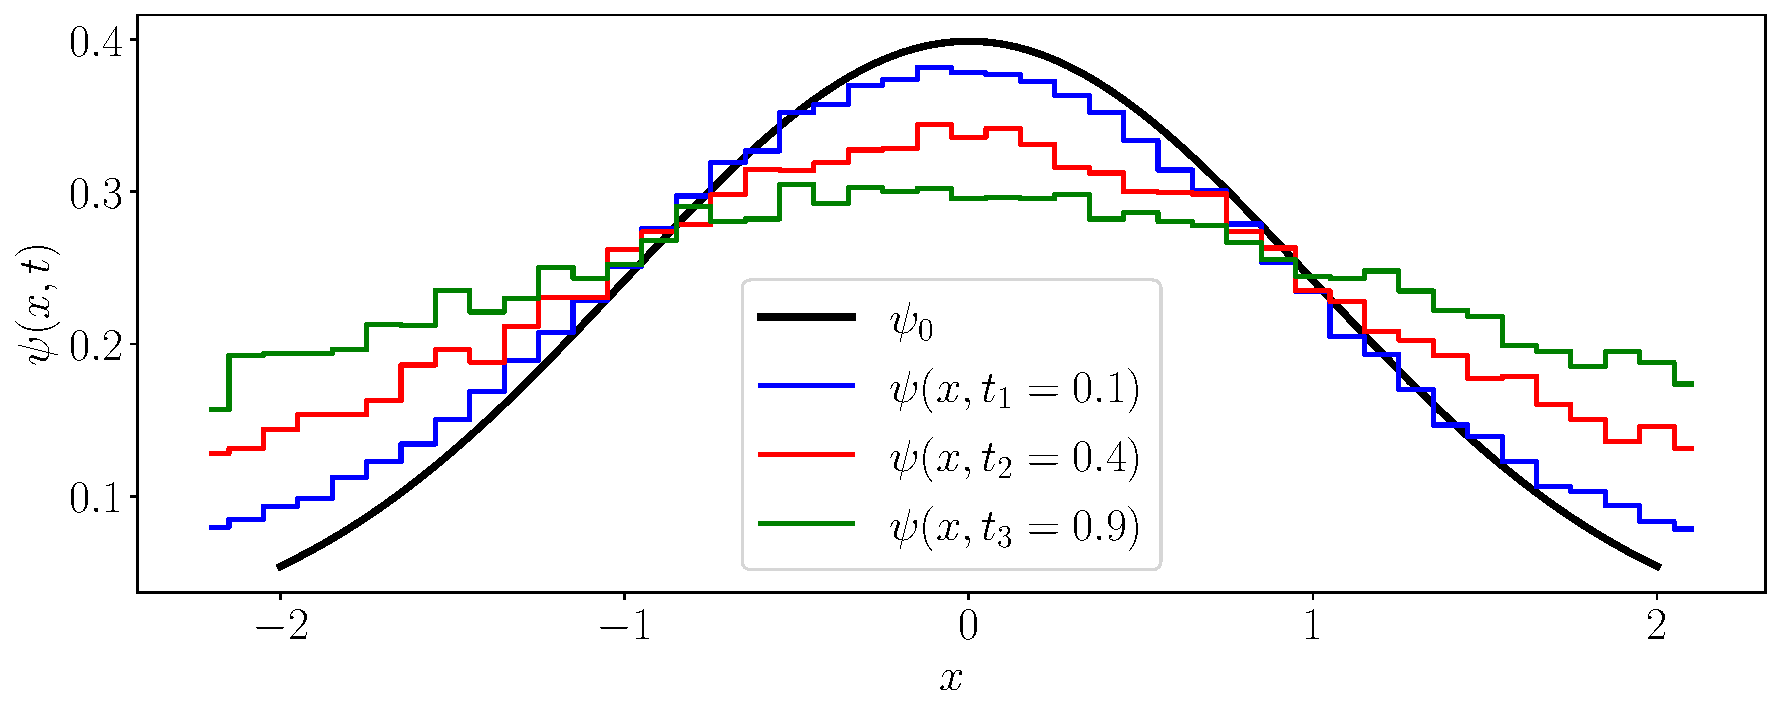
\includegraphics[width = \linewidth]{Chapter3/Figs/Raster/fkac_vs_fplanck_bottom.pdf}}
	
	\caption[Feynman-Kac for a free particle in 1D]{\textbf{Feynman-Kac for a free particle  in 1D.} \textbf{top:} $N=400$ Brownian walks starting from different $x_0$, the color signifies initial position. In order to evaluate $\psi$ between $x-\frac{\delta x}{2}$ and $x+\frac{\delta x}{2}$ at some time $t$ we must first find Brownian paths that end there. \textbf{middle:} The paths that pass through at $x \in (1.5, 1.6)$ (blue) and through $x \in (-0.4,-0.3)$ (red) are colored, others are left in grey. \textbf{bottom:} Time evolution of the initial condition $\psi_{0} = \frac{1}{\sqrt{2 \pi}} e^{-\frac{1}{2} x^{2}}$, by estimating ${\mathbb{E}}\left[\psi\left(X_{0}, 0\right)\right]$ from the filtered paths at each timestep.}
	\label{fig:fk_1d_example}
\end{figure}
\noindent
The role of the potential in the Feynman-Kac formula is to weight the Brownian paths, in turn defining the Feynman-Kac \emph{path measure} $\mathbb{P}_{\mathrm{FK}}$ it is related to the Brownian measure $\mathbb{P}_{0}$ by the Radon-Nykodym derivative
\begin{equation}
\label{eq:RNderiv}
\frac{\mathrm{d} \mathbb{P}_{\mathrm{FK}}}{\mathrm{d} \mathbb{P}_{0}}=\mathcal{N} \exp \left(-\int V\left(X_{t}\right) d t\right),
\end{equation}
where $\mathcal{N}$ is a normalizing constant. Intuitively we can understand the measure as assigning more weight to Brownian paths that spend more time in the attractive region ($V(x) < 0$) than in repulsive regions ($V(x) > 0$), this is illustrated in Fig.~\ref{fig:fkac_measure_reweight}.
\begin{figure}[h]
	\centering
	\subfloat{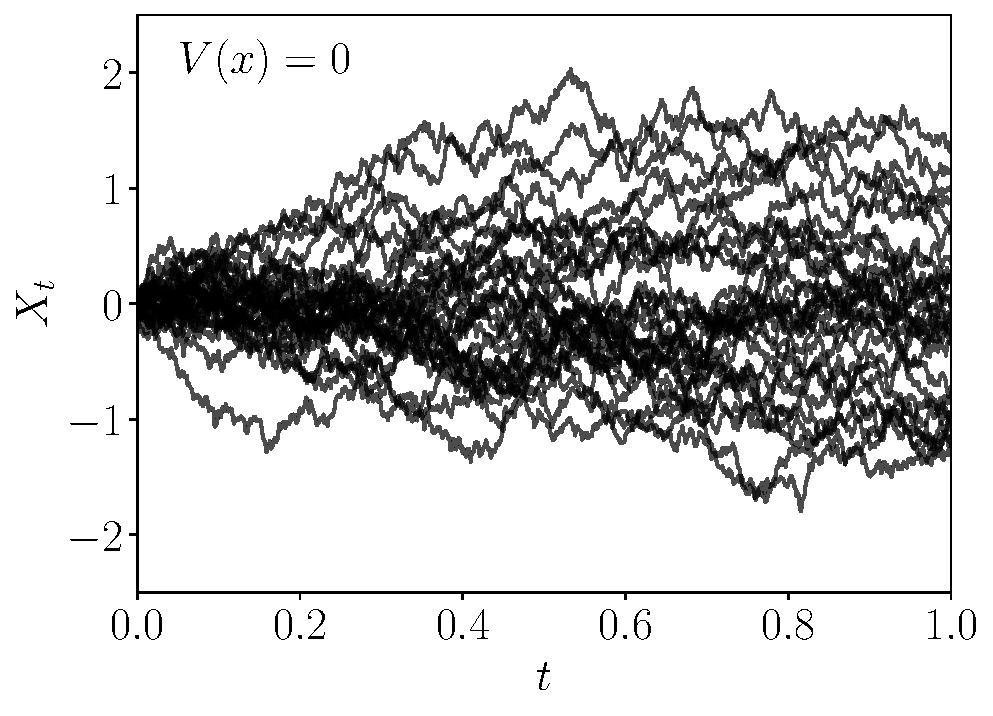
\includegraphics[width=0.5\linewidth]{Chapter3/Figs/Raster/reweight1.pdf}}
	\subfloat{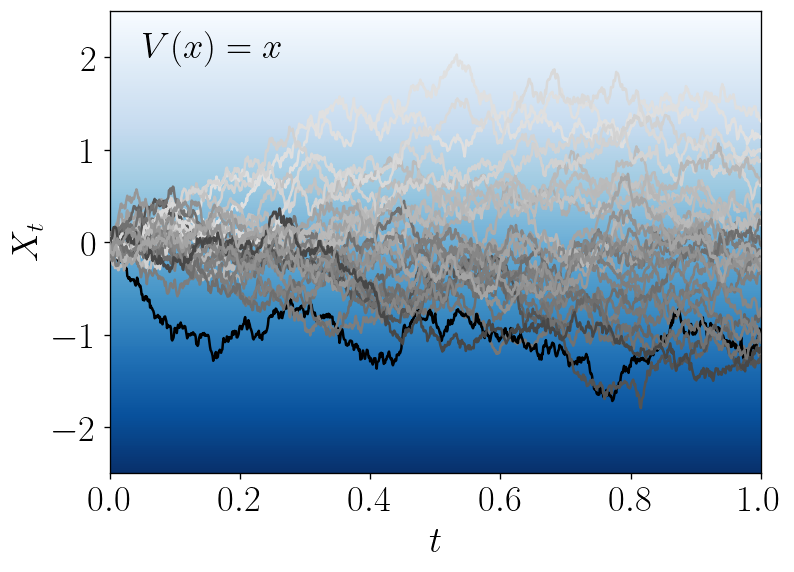
\includegraphics[width=0.5\linewidth]{Chapter3/Figs/Raster/reweight2.png}}
	\caption[Feynman-Kac measure in a linear potential]{\textbf{Feynman-Kac measure in a linear potential.} 
		\textbf{left:} $N=30$ Brownian paths. \textbf{right:} The paths colored ($P(\text{black})=1$, $P(\text{white})=0$) by their likelihood under the Feynman-Kac measure with $V(x)=x$.}
	\label{fig:fkac_measure_reweight}
\end{figure}
Moreover, this new stochastic process is Markovian, meaning that a clear connection exists between the imaginary time Schr\" odinger equation and a SDE of form~\eqref{eq:SDE_general} with time-homogeneous $\sigma$ and $v$.
Indeed, in the continuous case we have discussed so far, the mapping between the Fokker-Planck equation~\eqref{eq:Fokker-Planck-General} and the Schr\" odinger equation exists in the form of a similarity transform. Starting from the FP equation of a stochastic process with constant volatility $\sigma = 1$
\begin{equation}
\label{eq:not_prime_cont_process}
\mathrm{d} X_{t}=\mathrm{d} W_{t}+v\left(X_{t}\right) \mathrm{d} t,
\end{equation} 
and drift $v(x)=-U^\prime(x)$ given as a gradient of some potential function $U(x)$, the PDF $\rho(t, x)$ of the process is
\begin{equation}
\frac{\partial \rho}{\partial t} = \frac{\partial}{\partial x}\left[\frac{\partial \rho}{\partial x}+U^{\prime}(x) \rho\right].
\end{equation}
We can define the function 
\begin{equation}
\psi(x, t)=\frac{\rho(x, t)}{\sqrt{\rho_{0}(x)}},
\end{equation}
with $\rho_{0}$ being the stationary distribution of the FP equation
\begin{equation}
\frac{\partial}{\partial x}\left[\frac{\partial \rho}{\partial x}+U^{\prime}(x) \rho\right] = 0 \quad \rightarrow \quad \rho_{0}(x) \propto \exp (-U(x)),
\end{equation}
which satisfies the imaginary time Schr\" odinger equation~\eqref{eq:imag_sch} with the Hamiltonian
\begin{equation}
\hat H=-\frac{\partial^{2}}{\partial x^{2}} \overbrace{-\frac{U^{\prime \prime}}{2}+\frac{U^{\prime 2}}{4}}^{\equiv V(x)}.
\end{equation}
The ground state of this Hamiltonian has zero energy and is 
\begin{equation}
\psi_{0}(x)=\sqrt{\rho_{0}(x)}.
\end{equation}
In other words, the quantum ground state probability distribution $|\psi_{0}|^2$ is the same as classical stationary distribution $\rho_{0}$ of the stochastic process $X_{t}$ in the literature referred to as the \emph{Nelson's ground state process}~\cite{nelson1967dynamical, albeverio1977energy}. This connection is one that our computational method will exploit, as the ability to efficiently sample from the stochastic process with correct drift $v$ is equivalent to sampling from the ground state of the quantum system. Even though the connection is simple, it comes with a caveat. Starting from the Schr\" odinger equation one needs to find the drift $v(x)$ and while the connection with the potential of the Hamiltonian is clear-cut in this simple example, this is not the case in many-body systems, i.e. the \emph{inverse problem} of finding the stochastic process of a given Hamiltonian is difficult, and is one of the core problems approached in this thesis.

\subsection{Stoquastic Hamiltonians and Feynman-Kac in discrete state space}
\label{subsec:fk-latt}
Before we illustrate the connection between the imaginary time Schr\" odinger equation and CTMCs we must introduce \textbf{Stoquastic Hamiltonians}~\cite{bravyi2006complexity}, a class of Hamiltonians which do not suffer from the sign problem.
\begin{definition}[Stoquastic Hamiltonian]
	A $k$-local Hamiltonian $\hat H=\sum_{i} \hat H_{i}$ is \textbf{stoquastic} if there exists a local basis $\mathcal{B}$ in which off-diagonal matrix elements of terms $\hat{H}_i$ are zero or negative
	\begin{equation}
		\langle x|\hat H| y\rangle \leq 0, \quad \forall x, y \in \mathcal{B} \text {\quad with } x \neq y.
	\end{equation}
\end{definition}
\noindent
If we consider the matrix $e^{-\tau \hat H}$ for a non-positive $\hat H$, we see that every term in the expansion
\begin{equation}
	e^{-\tau \hat{H}} = 1 -\tau \hat{H} + \frac{1}{2}(\tau \hat{H})^2 + \ldots
\end{equation}
is a non-negative matrix, thus so is $e^{-\tau \hat H}$. In the infinite time limit, the ground state is projected out
\begin{equation}
	\lim _{\tau \rightarrow \infty} e^{-\tau \hat H}=|\psi_0\rangle\langle\psi_0|, 
\end{equation}
and a global phase exists for which the ground state has non-negative amplitudes. Moreover, if $\hat H$ is irreducible then the ground state is node-less~\cite{discussion_stoquastic2017}
\begin{equation}
	\psi_0(x)>0 \text { for all } x \in \mathcal{B}.
\end{equation}
We can decompose a stoquastic Hamiltonian into a rate matrix $\Gamma$, as defined in section~\ref{subsubsect:CTMC}, and a diagonal potential matrix $V$
\begin{equation}
	\label{eq:hamilton_split}
	H=-\Gamma+V.
\end{equation}
The rates $\Gamma$ are analogous to the Brownian motion in the continuum case, or can be interpreted as the kinetic contribution. They represent a CTMC which we will understand as \emph{passive dynamics}. In terms of the Hamiltonian matrix,
\begin{equation}
\Gamma_{s \rightarrow s^{\prime}}=\left\{\begin{array}{ll}
-H_{s s^{\prime}} & \text { if } s \neq s \\
\sum_{s^{\prime} \neq s} H_{s s^{\prime}} & \text { if } s=s^{\prime}
\end{array}\right.
\end{equation}
and the potential is
\begin{equation}
V(\boldsymbol{s})=H_{s s}+\sum_{s^{\prime} \neq s} H_{s s^{\prime}}.
\end{equation}
From now on we use $\rightarrow$ notation to emphasise the transition between \emph{adjacent} states $s\neq s^\prime$ which satisfy $H_{s s^{\prime}} \neq 0$. This decomposition allows us to define the Feynman-Kac formula in the discrete state space~\cite{rogers2000diffusions} as
\begin{equation}
	\label{eq:fkac_disc}
	\psi\left(s_t, t\right)=
	\underset{\Sigma_{[0, t] \sim \Gamma}}{\mathbb{E}}
	\left[
	\exp \left(-\int_{0}^{t} V\left(\boldsymbol{s}_{t^{\prime}}\right) \mathrm{d} t^{\prime}\right) \psi\left(s_0, 0\right)
	\right].
\end{equation}
The expectation is now taken over the process driven by $\Gamma$ and weighted by the potential $V$. We denote the trajectory as $\Sigma_{[0, t]}$, where $\Sigma_{t^\prime}$ is the state of the system at time $t^\prime \in [0, t]$. Analogous as with the Feynman-Kac formula in continuous state space, this defines a new CTMC with measure $\mathbb{P}_{\text{FK}}$, which is related to  passive dynamics with measure $\mathbb{P}_0$ by the RN derivative, eq.~\eqref{eq:RNderiv}.

How exactly is this CTMC connected to the imaginary time Schr\" odinger equation? The connection exists, as in the continuous space, via a similarity transform. The difference being that instead of Fokker-Planck we use the master equation to describe the time evolution of the pdf $P$
\begin{equation}
\frac{\partial P(s)}{\partial t}=\sum_{s^\prime \neq s}\left[\Gamma_{s^\prime \rightarrow s} P(s^\prime)-\Gamma_{s \rightarrow s^\prime} P(s)\right].
\end{equation}
The stationary state $P_0$ of the master equation satisfies detailed balance
\begin{equation}
	\Gamma_{k \rightarrow j}=\exp \left(\frac{V_{s^\prime}-V_{s}}{2}\right),
\end{equation}
and is thus
\begin{equation}
	P_{0}(s) \propto \exp \left(-V_{s}\right).
\end{equation}
The wave function 
\begin{equation}
	\psi(s, t)=\frac{P_{s}(t)}{\sqrt{P_{0}(s)}},
\end{equation}
then satisfies the imaginary time Schr\" odinger equation with the Hamiltonian
\begin{equation}
	\hat H_{s^\prime s}=\left\{\begin{array}{ll}
	-P_{0}^{-\frac{1}{2}}(s) \Gamma_{s^\prime \rightarrow s} P_{0}^{\frac{1}{2}}(s^\prime)=-1 & s^\prime \neq s \\
	\sum_{s^\prime \neq s} \Gamma_{s \rightarrow s^\prime} & s^\prime=s.
	\end{array}\right. 
\end{equation}
Again this Hamiltonian has a zero-energy ground state 
\begin{equation}
	\psi_{0}(s)=\sqrt{P_{0}(s)} \propto \exp \left(-\frac{V_{s}}{2}\right),
\end{equation}
we see that the quantum probability in the ground state $|\psi_0(s)|^2$ coincides with the stationary distribution of the CTMC. The connection in the direction from the Markov process to Hamiltonian is clear, but we are interested in the inverse, starting from the Hamiltonian and finding for the corresponding stochastic process. We now turn our attention towards defining a suitable optimisation objective that, when optimised, will yield the correct Markov process.

%********************************** % New Section  *************************************
\section{Control theoretic approach to QM and loss functions}
\subsection{Holland Cost in continuous space}
In section~\ref{subsec:FK_in_continuous_space} we explored a connection between the ground state of some quantum system and It\^ o processes. We have seen that the ground state probability $|\psi_0|^2$ is also the stationary distribution $\pi$ of some stochastic process
\begin{equation}
	\label{eq:holl_opt_process}
	\mathrm{d} X_{t}=\mathrm{d} W_{t}+v^\prime\left(X_{t}\right) \mathrm{d} t,
\end{equation}
where $v^\prime$ is the \emph{optimal}/correct drift. Finding the correct drift in one-dimension was straightforward, but how to do it in higher dimensions ($W_{t}, X_{t} \in \mathbb{R}^n$ and $v: \mathbb{R}^n \rightarrow \mathbb{R}^n$) remained unanswered. Holland~\cite{holland1977cost} formulated the search for optimal rates as a stochastic control problem with cost function
\begin{equation}
	\label{eq:holland_cost}
	C[v]=\lim _{T \rightarrow \infty} \frac{1}{T} \mathbb{E}\left[\int \left(\frac{1}{2}\left|v\left(X_{t}\right)\right|^{2}+V\left(X_{t}\right)\right)\mathrm{d} t\right],
\end{equation}
where the expectation is over the process in eq.~\eqref{eq:holl_opt_process}. Its derivation and proof of an unique solution can be found in Appendix~\ref{app:holland-cost}. To see that the minimum of $C[v]$ really corresponds to the ground state, we first rewrite the cost in terms of the stationary distribution $\pi(x | v)$ of It\^ o process generated by the drift $v$
\begin{equation}
C[v]=\int \left[\frac{1}{2}\left|v\left(X_{t}\right)\right|^{2}+V\left(X_{t}\right)\right] \pi(x \mid v)\mathrm{d}x.
\end{equation}
The distribution $\pi$ must satisfy the stationary Fokker-Planck equation
\begin{equation}
\frac{1}{2} \nabla^{2} \pi-\nabla \cdot(v \pi)=0,
\end{equation}
the equation holds for drift $v = \frac{\nabla \psi}{\psi}$ and distribution $\pi = \psi^2$, the cost is then
\begin{equation}
C[v]=\int \left[\frac{1}{2}(\nabla \psi)^{2}+V\left(X_{t}\right) \psi^{2}\right]\mathrm{d}x.
\end{equation}
For normalised $\psi$ the integrand is the expected value of the quantum energy of the system, its minimum value $\lambda$ is the ground state energy $E_0$ and is achieved for the ground state wave function $\psi_{0}$. We could directly use the Holland's cost to find the optimal rates $v^\prime$, but we will instead use the fact that trajectories sampled under the Feynman-Kac measure $\mathbb{P}_{\mathrm{FK}}$ coincide with ones sampled from the optimal drift, and base our variational approach on finding the FK measure.

\subsection{Loss for continuous state space}
\label{subsec:continuous_loss}
To see that the path measures $\mathbb{P}_v$ of the process in eq.~\eqref{eq:not_prime_cont_process}  and the Feynman-Kac measure $\mathbb{P}_{\mathrm{FK}}$ coincide for the optimal rates $v^\prime$, we first need a measure of similarity between probability distributions. For this purpose we will use the \textbf{Kullback–Leibler} divergence $D_{\mathrm{KL}}$
\begin{equation}
	D_{\mathrm{KL}}(p \| q)=\underset{p}{\mathbb{E}}\left[\log \left(\frac{p}{q}\right)\right],
\end{equation}
the quantity is a divergence because of the asymmetry $D_{\mathrm{KL}}(p \| q) \neq D_{\mathrm{KL}}(q \| p)$. It is a strictly positive quantity $D_{\mathrm{KL}}(p \| q) \geq 0$ except for $p = q$ when $D_{\mathrm{KL}}(p \| q) = 0$. In order to obtain the KL divergence between $\mathbb{P}_v$ and $\mathbb{P}_{\mathrm{KL}}$ we first express the RN derivative of each path measure w.r.t. Brownian motion using Girsanov theorem~\eqref{eq:Girsanov_theorem}. Both RN derivatives can then be combined to express the logarithm Radon-Nikodym derivative or the \emph{log-likelihood} ratio as
\begin{equation}
\log \left(\frac{d \mathbb{P}_{v}}{d \mathbb{P}_{\mathrm{FK}}}\right)=
\tilde{\ell}-
E_{0} T+
\log 
\left(
\frac{\varphi_{0}\left(r_{0}\right)}{\varphi_{0}\left(r_{T}\right)}
\right),
\end{equation}
where we have defined $\tilde{\ell}$ as
\begin{equation}
\tilde{\ell} \equiv \int v\left(r_{t}\right) \mathrm{d} W_{t}+\int \left(\frac{1}{2}\left|v\left(r_{t}\right)\right|^{2}+V\left(r_{t}\right)\right)\mathrm{d} t.
\end{equation}
The boundary term depends the ground state $\varphi_0$ at initial $r_0$ and final $r_T$ points in the trajectory, and originates from the normalisation constant $\mathcal{N}$ in the Radon-Nikodym derivative. The KL divergence is 
\begin{equation}
\label{eq:ltilde-cont}
D_{\mathrm{KL}}\left(\mathbb{P}_{v} \| \mathbb{P}_{\mathrm{FK}}\right)=\underset{\mathbb{P}_{v}}{\mathbb{E}}\left[\ell^\prime-E_{0} T+\log \left(\frac{\varphi_{0}\left(r_{0}\right)}{\varphi_{0}\left(r_{T}\right)}\right)\right].
\end{equation}
If we consider the above Kullback-Leibler divergence in the long time limit $T \rightarrow \infty$, we see that the expectation of the first term of $\tilde{\ell}$ is zero. Moreover, if the marginal distributions $\psi_{0}(r_0)$ and $\psi_{0}(r_T)$ coincide, the boundary term vanishes as well and the KL divergence is equivalent to the Holland cost, thus vanishes for optimal drift. This means that finding the correct path measure is equivalent to finding the optimal drift, and in standard machine learning fashion, minimizing $D_{\mathrm{KL}}$ can be used to find the optimal rates. Sampling the trajectories becomes a matter of integrating a SDE and can be done with some standard approach, e.g. Euler-Mayurama method. The rates $v_{\theta}$ are parameterised and gradients of $D_{\mathrm{KL}}$ w.r.t $\theta$ can be obtained using stochastic backpropagation where the reparameterisation trick is used for each increment in the discretised SDE. The gradient of the boundary term is non-zero, but it can be estimated by expressing $\psi_0$ in terms of $v_{\theta}$. Missing steps of the derivation can be found in Appendix~\ref{app:holland-prob}, more details in~\cite{barr2020quantum}. 

\subsection{Todorov Cost in discrete state space}
We now turn our attention towards finding a variational approach in discrete state space and continuous time. We rely on foundational work done on linearly solvable Markov Decision Processes\footnote{For a general discussion of MDP's see~\cite{sutton2018reinforcement}} (MDP) by Todorov~\cite{todorov2007linearly, todorov2009efficient} and its applications to lattice problems~\cite{gispen2020ground}. The main idea is to reinterpret the dynamics of the imaginary time Schr\" odinger equation in the Todorov MDP framework by treating control as a modification of the passive dynamics of the system. The imaginary time Schr\" odinger equation can be written as
\begin{equation}
	\label{eq:sch_split}
	\frac{\partial \psi(s_j, t)}{\partial t}=-\underbrace{\sum_{s_k \neq s_j} \Gamma_{s_j \rightarrow s_k}\left[\psi(s_k, t)-\psi(s_j, t)\right]}_{\text{passive dynamics}}
	-V_{s_j} \psi(s_j, t)
\end{equation}
to emphasise the decomposition of the Hamiltonian eq.~\eqref{eq:hamilton_split} into passive dynamics and the potential. Akin to the transformation in discrete space, we use $\psi(s_j, t)=\exp[-u(s_j, t)]$, to arrive at an alternative form
\begin{equation}
	\label{eq:bellman_sch}
	-\frac{\partial u(s_j, t)}{\partial t}=\min _{\Gamma^{(v)}}\left[\ell(s_j, v)+\sum_{s_k} \Gamma_{s_j \rightarrow s_k}^{(v)}(u(s_k, t)-u(s_j, t))\right],
\end{equation}
where $\Gamma^{(v)}$ are the rates of the modified CTMC, and $\ell(s_j, v)$ is the cost per time associated with state $s_j$ and parameters $v$.
This is a form of Bellman equation, a very general concept in control theory and reinforcement learning, related to the Hamilton-Jacobi equation in physics, it is used to find the optimal actions i.e. how we should choose $v$ at each moment w.r.t the cost associated with each state and parameters $\ell(s_j, v)$. The function $u(s_j, t)$ is the cost-to-go function, it is the cumulative cost obtained starting from state $s_j$ at time $t$ and acting optimally afterwards. The optimal parameters $v(t)$ are computed greedily with each step and guarantee minimum $u(s_j, t)$, most easily illustrated by looking $\Delta t$ into the past, where the cost-to-go is given by the cost of remaining in the same state $\ell(s_j, t) \Delta t$ and the changes in costs-to-go when transitioning to other states weighted by the probability of making the transition $\Gamma^{(v)}_{s_j \rightarrow s_k}$
\begin{equation}
	u_{j}(t-\Delta t)=u_{j}(t)+\Delta t \min _{\Gamma^{(v)}}\left[\ell(j, v)+\sum_{k} \Gamma_{j \rightarrow k}^{(v)}(u(k, t)-u(j, t))\right].
\end{equation}
The cost $\ell(s_j, v)$ introduced by Todorov is of the form
\begin{equation}
	\ell(j, v)=q(j)+D_{\mathrm{KL}}(v(\cdot \mid j) \| p(\cdot \mid j)),
\end{equation}
where the first term encodes how undesirable different states are, and the second measures how costly the deviation from passive dynamics is, the agent (controlled rates) pay a price for reshaping the environment (passive rates), for more rigour see Appendix~\ref{app:todorov-cost}. In the case of the imaginary time Schr\" odinger equation, these terms are
\begin{equation}
	q(s_j)=V(s_j) \Delta t,
\end{equation}
and
\begin{equation}
	D_{\mathrm{KL}}=\underset{\Sigma_{[0, t]} = k_t \sim \Gamma^{(v)}}{\mathbb{E}}\left[\sum_{n} D_{\mathrm{IS}}\left(\Gamma_{k^{(n)} \rightarrow k^{(n+1)}}^{(v)}, \Gamma_{k^{(n)} \rightarrow k^{(n+1)}}\right)\right],
\end{equation}
where $\Sigma_{[0, t]}$ is the trajectory of states sampled from controlled dynamics $\Gamma^{(v)}$  which visits states $k^{(n)}$ for $t_{n-1} < t < t_{n}$ and $D_{\mathrm{IS}}$ is the Itakura-Saito divergence, see Appendix~\ref{app:todorov-cost}.

\subsection{Loss for discrete state space}
\label{subsec:discrete_loss}
As we have done in the continuous space, we will compare the cost to the Kullback-Liebler divergence of the two path measures $\mathbb{P}_v$ and $\mathbb{P}_{\mathrm{FK}}$ to see that the optimal rates $\Gamma^{(v)}$ coincide with sampling from the Feynman-Kac measure, full derivations in~\ref{app:todorov-prob}. The logarithm Radon-Nikodym between the controlled rates and Feynman-Kac measure is
\begin{equation}
	\label{eq:logrn-discrete}
	\log \left(\frac{\mathrm{d} \mathbb{P}_{v}}{\mathrm{d} \mathbb{P}_{F K}}(k(t))\right)
	= \tilde \ell
	+\sum_{n} \log \left(\frac{\Gamma_{k^{(n)} \rightarrow k^{(n+1)}}^{(v)}}{\Gamma_{k^{(n)} \rightarrow k^{(n+1)}}}\right)-E_{0} T-\log \left(\frac{\varphi(k^{(N)})}{\varphi(k^{(0)})}\right),
\end{equation}
where we have defined $\tilde \ell$ as
\begin{equation}
\tilde \ell = \int \left[V(k(t))+\sum_{l \neq k(t)}\left(\Gamma_{k(t) \rightarrow l}-\Gamma_{k(t) \rightarrow l}^{(v)}\right)\right] \mathrm{d}t.
\end{equation}
The KL divergence can be written as
\begin{equation}
	\begin{aligned}
		D_{\mathrm{KL}}\left(\mathbb{P}_{\nu} \mid \mathbb{P}_{\mathrm{FK}}\right) = \underset{P_{v}}{\mathbb{E}}\Bigg[\int V(k(t))&+\sum_{l \neq k(t)}\left(\Gamma_{k(t) \rightarrow l}-\Gamma_{k(t) \rightarrow l}^{(v)}\right)\\
		&+\Gamma_{k(t) \rightarrow l}^{(v)} \log \left(\frac{\Gamma_{k(t) \rightarrow l}^{(v)}}{\Gamma_{k(t) \rightarrow l}}\right) d t-\log \left(\frac{\varphi(k^{(N)})}{\varphi(k^{(0)})}\right)\Bigg]-E_{0} T,
	\end{aligned}
\end{equation}
which is the Todorov's cost and vanishes for optimal rates, meaning that finding the these rates is equivalent to finding the Feynman-Kac measured process. One might be tempted to use $D_{\mathrm{KL}}$ as an optimisation objective, but this is not possible because its gradient is biased due to the boundary term
$\log \left(\frac{\varphi(k^{(N)})}{\varphi(k^{(0)})}\right)$. We now propose two alternatives.

\subsubsection{Loss no. 1: Variance of $\tilde \ell$}
The variance of quantity $\tilde{\ell}$
\begin{equation}
	\tilde{\ell}=
	\log \left(\frac{\mathrm{d} \mathbb{P}_{v}}{\mathrm{~d} \mathbb{P}_{F K}}(k(t))\right)
	-\sum_{n} \log \left(\frac{\Gamma^{(v)}_{k^{(n)} \rightarrow k^{(n+1)}}}{\Gamma_{k^{(n)} \rightarrow k^{(n+1)}}}\right)
	+E_{0} T
	+\log \left(\frac{\varphi\left(k^{(N)}\right)}{\varphi\left(k^{(0)}\right)}\right)
\end{equation}
 can be used as a loss function. Kolmogorov's criterion tells us that
 \begin{equation}
 	\log \left(\frac{\Gamma_{k^{(n)} \rightarrow k^{(n+1)}}^{(v)}}{\Gamma_{k^{(n)} \rightarrow k^{(n+1)}}}\right)=\log \left(\frac{\varphi(k^{(n+1)})}{\varphi(k^{(n)})}\right),
 \end{equation}
 combined with the fact that the Radon-Nikodym derivative is $0$ for correct transition rates $\Gamma^{(v)} = \Gamma^\prime$ means that $\operatorname{Var}[\tilde{\ell}]$ vanishes in that case, moreover it is bounded below by zero making it a suitable objective function. \hl{TODO: fix, For optimal rates $\tilde \ell$ is equal to $E_0 T$ and is an estimator of the ground state energy.}
 
\subsubsection{Loss no. 2: Variance of log Radon-Nikodym derivative with fixed endpoints}
While the gradients of $D_{\mathrm{KL}}\left(\mathbb{P}_{\nu} \mid \mathbb{P}_{\mathrm{FK}}\right)$ are \hl{change this sentance} biased, we can still make use of the logarithm RN derivative~\eqref{eq:logrn-discrete}. It vanishes for optimal rates and while we can treat $E_0 T$ as constant, we have no easy way to approximate the wave function $\varphi$ in the boundary term which in general does not have zero variance. We can exploit the fact that log RN must be constant on all trajectories and consider a batch of trajectories with fixed endpoints, in this case the variance of the boundary term vanishes. How to obtain such a batch poses a technical challenge which is to be solved on a system by system basis, usually by generating a single trajectory and perturbing it in such a way that one obtains many paths with fixed endpoints.


%********************************** % Ch3 Nomenclature *************************************
\nomenclature[Z-sde]{SDE}{Stochastic Differential Equations}
\nomenclature[Z-RN]{RN}{Radon-Nikodym}
\nomenclature[Z-fp]{FP}{Fokker-Planck}
\nomenclature[z-pdf]{pdf}{Probability density function}
\nomenclature[z-cdf]{cdf}{Cumulative density function}
\nomenclature[z-stochprocs]{s.p.}{Stochastic process}
\nomenclature[z-dtmc]{DTMC}{Discrete time Markov Chain}
\nomenclature[z-ctmc]{XTMC}{Continuous time Markov Chain}
\nomenclature[z-mdp]{mdp}{Markov Decision Process}

\nomenclature[x-ratematrix]{$\Gamma$}{Transition rate matrix}
\nomenclature[x-kldiv]{$D_{\mathrm{KL}}$}{Kullback-Liebler divergence}
\nomenclature[x-statespace]{S}{State space of a Markov process}
\nomenclature[x-reals]{$\mathbb{R}$}{The set of real numbers}
\nomenclature[x-normal]{$\mathcal{N}$}{The Gaussian distribution}
\nomenclature[x-measure]{$\mathbb{P}$}{Measure}
\nomenclature[x-filtration]{$\mathbb{F}$}{Filtration}
\nomenclature[x-field]{"$\mathcal{F}$"}{$\sigma$-field (algebra)}
\nomenclature[x-stochprocs]{$\{X_t\}$}{Stochastic process}
\nomenclature[x-randomvariable]{$\{X\}$}{Random variable}
\nomenclature[x-wiener]{$W_t$}{Wiener process, mathematical Brownian motion}

%!TEX root = ../thesis.tex
% **************************** Define Graphics Path **************************
\ifpdf
\graphicspath{{Chapter4/Figs/Raster/}{Chapter4/Figs/PDF/}{Chapter4/Figs/}}
\else
\graphicspath{{Chapter4/Figs/Vector/}{Chapter4/Figs/}}
\fi


%*******************************************************************************
%****************************** Fourth Chapter *********************************
%*******************************************************************************

\chapter{Methodology}
\label{chapter4}
This chapter presents the computational method developed in this thesis. We start by introducing each component of the method separately before presenting how they fit together into a single procedure. We discuss neural networks, automatic differentiation, gradient estimation, gradient-based optimisation, as well as importance sampling. Finally, we present the actual implementation in \emph{JAX}, and discuss computational considerations and intricacies of thereof.

\section{Neural Networks} % ~150 words
The field of Machine learning has been going through a renaissance in the past decade, mainly due to the spark ignited by an increase in computational power and the advent of deep learning~\cite{goodfellow2016deep}. In this section we give only the bare necessities needed to understand the the method developed in this thesis. We introduce basic concepts, the multilayer perceptron, convolutional layers, and discuss the role symmetry plays in designing neural networks for a task and why it is important in applications to lattice models.  
\hl{todo, model + learning algorithm = learning etc.}

\newpage
\subsection{The Multilayer Perceptron} % saturday morning
The \textbf{multilayer perceptron} (MLP), also referred to as a \textbf{deep feedforward network} or simply a \textbf{deep neural network} (DNN), is the paradigmatic model of deep learning and serves as a foundation of more advanced models. In essence it is nothing more than a mapping of inputs to outputs
\begin{equation}
	f(\mathbf{x}; ~\theta): \mathbb{R}^\text{in} \rightarrow \mathbb{R}^{\text{out}},
\end{equation}
which is structured in a certain way and depends on parameters $\theta$. The mapping is a composition of vector-valued functions $f$ which are called \emph{layers} of the network, and with each layer we associate variational parameters $\mathbf{w}$, or simply the weights. The MLP can be described with a directed acyclic graph which details the compositions of the layers. The simplest and most common is a chain of compositions, Fig~\ref{fig:mlp}b, 
\begin{equation}
f_{\text{MLP}} = \left(f^{(n)} \circ f^{(n-1)} \circ \cdots \circ f^{(2)} \circ f^{(1)} \right)(\mathbf{x}),
\end{equation}
where the input $\textbf{x}$ passes through \emph{hidden layers} before the \emph{output layer} outputs the result. The length of this chain is the \emph{depth} of the network, and the dimensionality of hidden layers is the \emph{width} of the network. We can interpret each transformation $f^{(i)}$ as consisting of a unit/node/neuron for each input dimension, which is vector-to-scalar transformation, Fig~\ref{fig:mlp}a.
\begin{figure}[h]
	\centering
	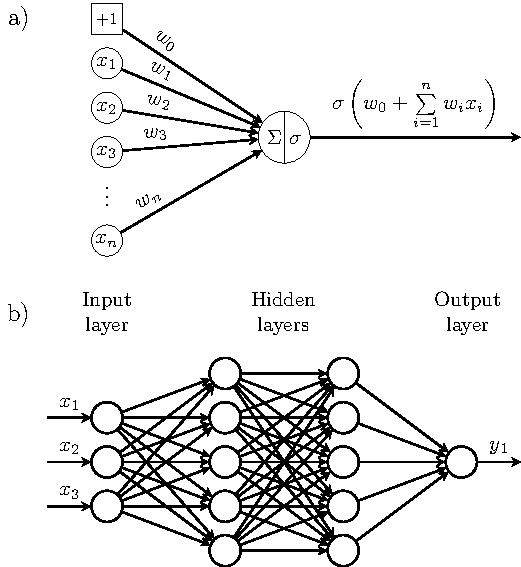
\includegraphics[width=\linewidth]{Chapter4/Figs/Vector/mlp.pdf}
	\caption[Multilayer Perceptron]{\textbf{Multilayer Perceptron.} \textbf{top: }A node outputs the activation function $\sigma$ evaluated at the weighted average over outputs from the previous layer and bias. \textbf{bottom: } A MLP with two hidden layers ($f^{(1)}: \mathbb{R}^3 \rightarrow \mathbb{R}^4$, $f^{(2)}: \mathbb{R}^4 \rightarrow \mathbb{R}^4$, $f^{(3)}: \mathbb{R}^4 \rightarrow \mathbb{R}$).}
	\label{fig:mlp}
\end{figure} 
The simplest layer would be a linear one, composed of
\begin{equation}
f(\mathbf{x}; \mathbf{w}, b) = \mathbf{x}^\intercal \mathbf{w} + b.
\end{equation}
However, a linear neural network famously cannot learn the XOR function~\cite{minsky2017perceptrons}, and in practice a nonlinearity or \emph{activation} function $g$ is used in each node to bolster the network's representational power
\begin{equation}
f(\mathbf{x}; \mathbf{w}, b) = g\left(\mathbf{x}^\intercal \mathbf{w} + b\right).
\end{equation}
A variety of activations has been used, namely $\tanh(\cdot)$ and the logistic sigmoid $\sigma(\cdot)$, but have since been displaced by the use of the \textbf{rectified linear unit} or $\operatorname{ReLu}(\cdot)$, which is advantageous for training, for the output layer we will use the \emph{softplus}, which fulfils the requirement of being positive everywhere, Fig.~\ref{fig:activations}. A multilayer perceptron is a \textbf{universal function approximator}, meaning that with at least one hidden layer it can approximate any Borel measurable function mapping from a finite-dimensional space to another with desired accuracy, given enough hidden units~\cite{leshno1993multilayer}. 
\begin{figure}[H]
	\centering
	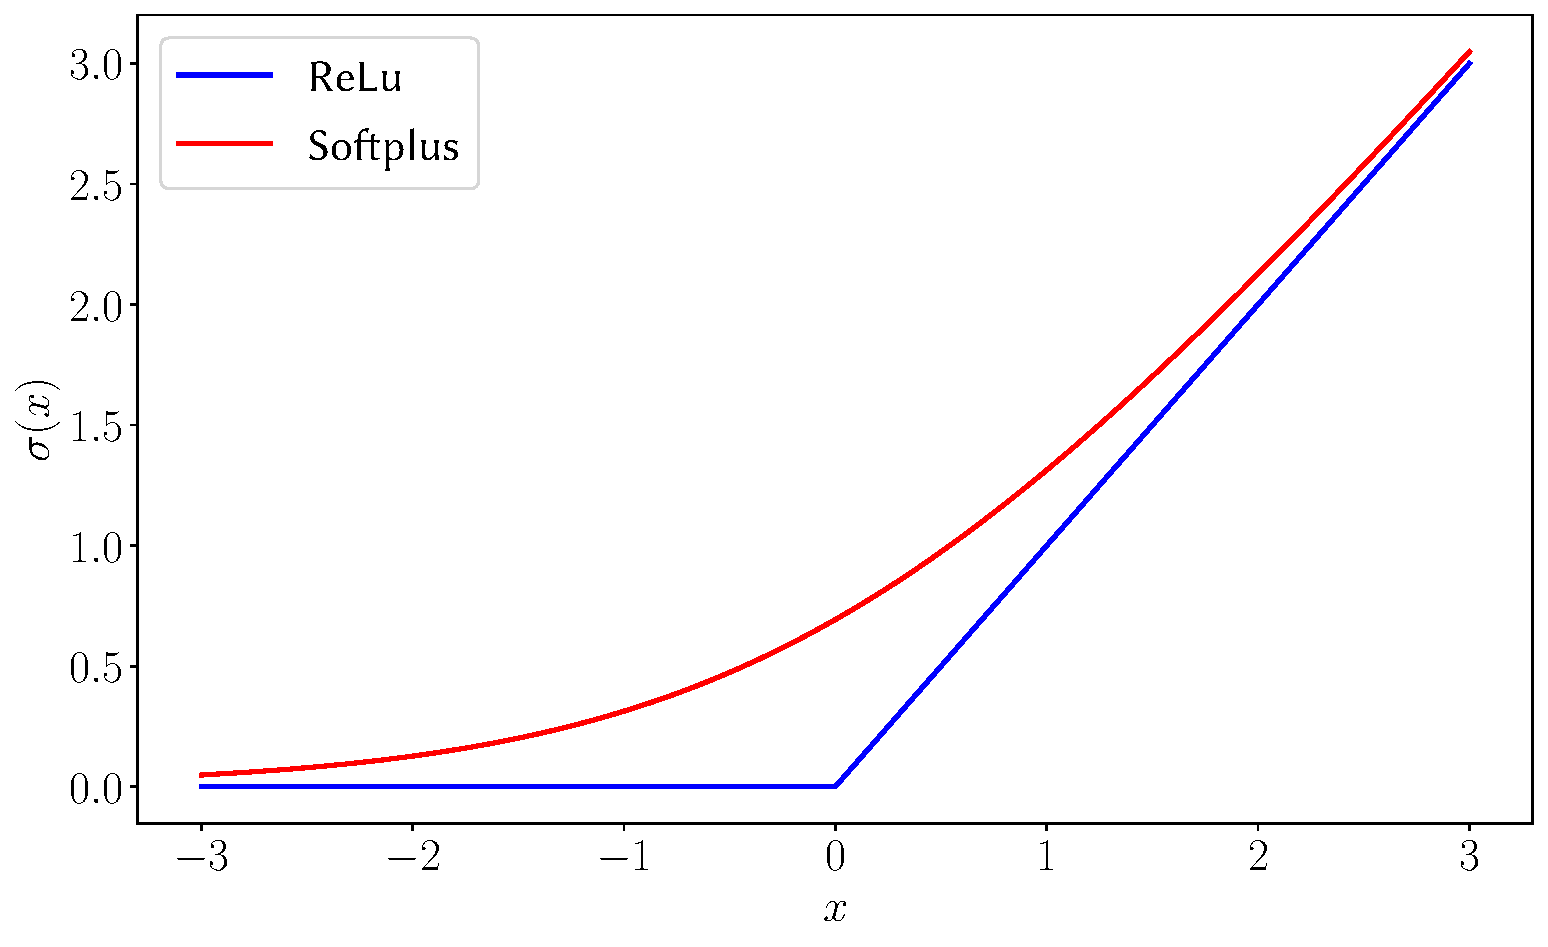
\includegraphics[width=\linewidth]{Chapter4/Figs/Vector/activations}
	\caption[Activation functions]{\textbf{Activation functions.} $\operatorname{ReLu}$ and Softmax activation functions.}
	\label{fig:activations}
\end{figure}

\newpage
\subsection{Convolutional Neural Networks} % saturday morning
\label{subsec:nn-cnn}
convolutional layer, pool layer, etc. 

\subsubsection{Periodic CNN}
periodic padding

\begin{figure}[H]
	\centering
	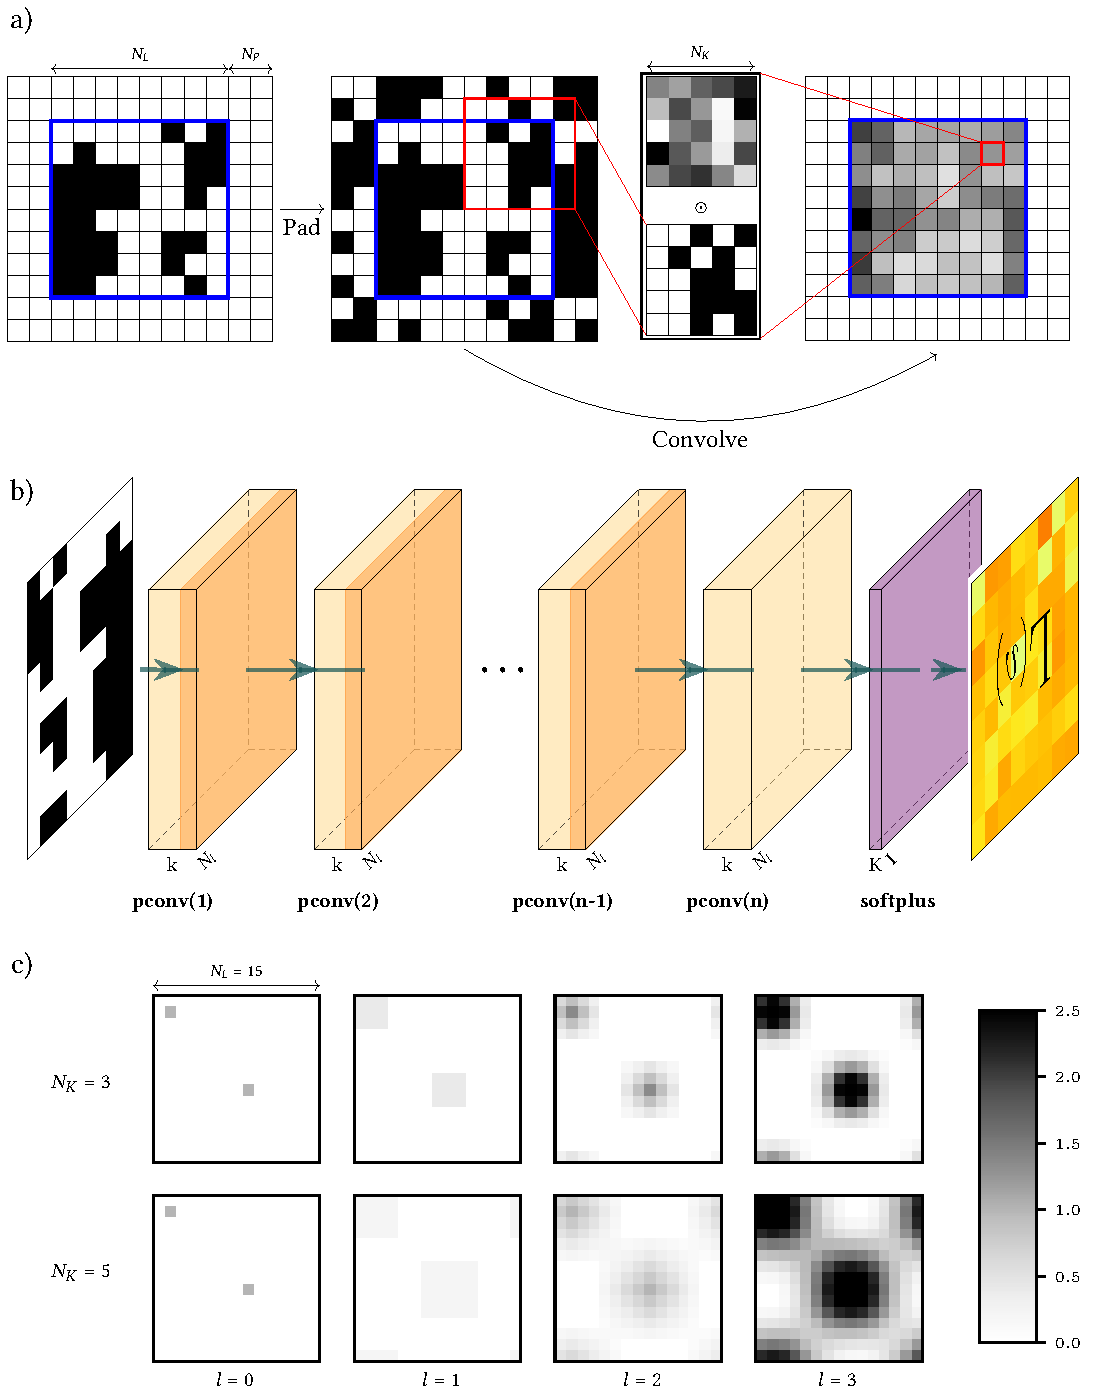
\includegraphics[width=\linewidth]{../diagrams/pcnn/pcnn}
	\caption[Periodic CNN]{\textbf{Periodic CNN}}
	\label{fig:pcnn}
\end{figure}

\subsubsection{Encoder-Decoder CNN} % saturday morning
skip connections, literature where it is used

\subsubsection{Group Equivariant CNN} % saturday eveninig
intro of about 400 words, following group equivariant CNN paper, and 

\newpage
\section{Monte Carlo Importance Sampling}
\label{sec:Impl-MCIP}
The most common application of Monte Carlo methods is evaluation of integrals in high dimensional space. There MC has a distinct advantage over quadrature methods, as the statistical error decreases with the square root of samples irregardless of the dimensionality of the problem. Integrals of a function $g(\mathbf{R})$
\begin{equation}
I=\int g(\mathbf{R}) \mathrm{d} \mathbf{R},
\end{equation}
where $\mathbf{R}$ is the \emph{configuration} of the system or simply a \emph{walker}, can be integrated by use of an \emph{importance function} $\mathrm{P}(\mathbf{R})$, where $\int d \mathbf{R} \text{P}(\mathbf{R})=1$ and $\mathrm{P} (\mathbf{R}) \geq 0$. The integral can be rewritten in the form
\begin{equation}
\int g(\mathbf{R}) \mathrm{d} \mathbf{R} = \int \frac{g(\mathbf{R})}{\mathrm{P}(\mathbf{R})} \mathrm{P}(\mathbf{R}) \mathrm{d} \mathbf{R} = \int f(\mathbf{R})\mathrm{P}(\mathbf{R}) \mathrm{d} \mathbf{R},
\end{equation}
where $f(\mathbf{R}) = g(\mathbf{R}) / \mathrm{P}(\mathbf{R})$.
The importance function $\mathrm{P}(\mathbf{R})$ can be interpreted as a probability density. If we generate an infinite number of random uncorrelated configurations $\mathbf{R}_m$ from the distribution $\mathrm{P}(\mathbf{R})$, the sample average is a good estimator of the integral $I$
\begin{equation}
I=\lim _{M \rightarrow \infty}\left\{\frac{1}{M} \sum_{m=1}^{M} f\left(\mathbf{R}_{m}\right)\right\},
\end{equation}
and for an approximation with a finite number of samples
\begin{equation}
I \approx \frac{1}{M} \sum_{m=1}^{M} f\left(\mathbf{R}_{m}\right).
\end{equation}
Under conditions where the central limit theorem holds~\cite{foulkes2001quantum}, the estimator is normally distributed with variance $\sigma_{f}^{2}/M$, which can also be estimated from the samples as
\begin{equation}
\frac{\sigma_{f}^{2}}{M} \approx \frac{1}{M(M-1)} \sum_{m=1}^{M}\left[f\left(\mathbf{R}_{m}\right)-\frac{1}{M} \sum_{n=1}^{M} f\left(\mathbf{R}_{n}\right)\right]^{2}.
\end{equation}


\section{Metropolis-Hastings Algorithm}
\label{sec:Impl-MCMC}
The integration technique from the previous section relies on our ability to obtain samples from a probability distribution $\mathrm{P}(\mathbf{R})$. In the case of QMC these distributions are high-dimensional and cannot be directly sampled from. Moreover their normalisations are usually not known. 
The Metropolis-Hastings algorithm~\cite{hastings1970monte}, see Algorithm~1, avoids direct sampling from the distribution $\mathrm{P}(\mathbf{R})$ and is insensitive to its normalisation. It uses a Markov process whose stationary distribution $\pi(\mathbf{R})$ is the same as $\mathrm{P}(\mathbf{R})$	
to generate a sequence of configurations $\left\{\mathbf{R}_n\right\}_\mathrm{P}$ 
that are drawn from $\mathrm{P}(\mathbf{R})$. A Markov process is completely defined with its transition probability $\mathrm{P}(\mathbf{R} \rightarrow \mathbf{R}^\prime)$, which is the probability of transitioning from state $\mathbf{R}$ to state $\mathbf{R}^\prime$. For the process to have a unique stationary distribution two conditions must be met, the process must be \emph{ergodic} and it must obey \emph{detailed balance}
\begin{equation}
\mathrm{P}(\mathbf{R}) \mathrm P(\mathbf{R} \rightarrow \mathbf{R}^\prime) = \mathrm{P}(\mathbf{R}^\prime) \mathrm P(\mathbf{R}^\prime \rightarrow \mathbf{R}),
\end{equation}
rewritten as
\begin{equation}
\label{eq:detailed_balance}
\frac{\mathrm P ({\mathbf{R}})}{\mathrm P ({\mathbf{R}^\prime})} = \frac{\mathrm P(\mathbf{R}^\prime \rightarrow \mathbf{R})}{\mathrm P(\mathbf{R} \rightarrow \mathbf{R}^\prime)}.
\end{equation}
The right transition probability $\mathrm P(\mathbf{R} \rightarrow \mathbf{R}^\prime)$ is not known, but we can express it with a trial move transition probability $\mathrm{T}(\mathbf{R} \rightarrow \mathbf{R}^\prime)$ which we sample and acceptance probability $\mathrm{A}(\mathbf{R} \rightarrow \mathbf{R}^\prime)$ as
\begin{equation}
\mathrm P(\mathbf{R} \rightarrow \mathbf{R}^\prime) = \mathrm T(\mathbf{R} \rightarrow \mathbf{R}^\prime) \mathrm A(\mathbf{R} \rightarrow \mathbf{R}^\prime).
\end{equation}
For equation~\eqref{eq:detailed_balance} to hold, the acceptance probability must be 
\begin{equation}
A\left(\mathbf{R} \rightarrow \mathbf{R}^{\prime}\right)=\min \left(1, \frac{\mathrm{T}\left(\mathbf{R}^{\prime} \rightarrow \mathbf{R}\right) \mathrm{P}\left(\mathbf{R}^{\prime}\right)}{\mathrm{T}\left(\mathbf{R} \rightarrow \mathbf{R}^{\prime}\right) \mathrm{P}(\mathbf{R})}\right).
\end{equation}
Thus to sample from any probability distribution we need only have the ability to calculate probabilities $\mathrm P(\mathbf{R})$ and to sample from a trial transition probability $\mathrm T(\mathbf{R} \rightarrow \mathbf{R}^{\prime})$. The efficiency of the algorithm depends on the amount of trial moves that we reject. All trial moves would be accepted if $\mathrm{T}(\mathbf{R} \rightarrow \mathbf{R}^{\prime})= \mathrm{P}(\mathbf{R}^\prime)$, which would just mean sampling from $\mathrm P$ directly and is the very problem we are trying to solve with Metropolis-Hastings. 	
\begin{algorithm}
	\label{alg:MCMC}
	\SetAlgoLined
	\KwResult{A set of configurations $\left\{ \mathbf{R}_n \right\}_{\mathrm{P}}$ sampled from $\mathrm P$}
	Initialize walker at random configuration $\mathbf{R}$\;
	\While{no. samples less than $N$}{
		Generate new configuration $\mathbf{R}^\prime$ with transition probability $\mathrm{T}(\mathbf{R}\rightarrow\mathbf{R}^\prime)$\;
		
		Accept the move ($\mathbf{R} \rightarrow \mathbf{R}^\prime$) with probability $A\left(\mathbf{R} \rightarrow \mathbf{R}^{\prime}\right)=\min \left(1, \frac{\mathrm{T}\left(\mathbf{R}^{\prime} \rightarrow \mathbf{R}\right) \mathrm{P}\left(\mathbf{R}^{\prime}\right)}{\mathrm{T}\left(\mathbf{R} \rightarrow \mathbf{R}^{\prime}\right) \mathrm{P}(\mathbf{R})}\right)$\;
		
		Append $\mathbf{R}$ to the set of configuration;
	}
	\caption{Metropolis-Hastings}
\end{algorithm}

\section{Gradient based optimisation}
\label{sec:gbopt}

\subsection{Gradient estimation}
\label{subsec:gbopt-gest}

\begin{itemize}
	\item \textbf{TODO:} Rewrite with a more general tone, do not only talk about the ELBO. Still use Mohammeds review! It is very good.
\end{itemize}

In order to perform gradient descent on the ELBO objective, we need to be able to evaluate its gradients with respect to parameters $\boldsymbol{\theta}$ and $\boldsymbol{\phi}$. Taking the gradient w.r.t generative parameters $\boldsymbol{\theta}$ is straightforward, because we can change the order of the expectation operator and the gradient, leaving us with
\begin{equation}
\begin{aligned} 
\nabla_{\boldsymbol{\theta}} \mathcal{L}_{\boldsymbol{\theta}, \boldsymbol{\phi}}(\mathbf{x}) &=\nabla_{\boldsymbol{\theta}} 	\mathbb{E}_{q_{\boldsymbol{\phi}}(\mathbf{z} \mid \mathbf{x})}\left[\log p_{\boldsymbol{\theta}}(\mathbf{x}, \mathbf{z})-\log q_{\boldsymbol{\phi}}(\mathbf{z} | \mathbf{x})\right] \\  & \simeq \nabla_{\boldsymbol{\theta}}\left(\log p_{\boldsymbol{\theta}}(\mathbf{x}, \mathbf{z})-\log q_{\boldsymbol{\phi}}(\mathbf{z} | \mathbf{x})\right) \\ &=\nabla_{\boldsymbol{\theta}}\left(\log p_{\boldsymbol{\theta}}(\mathbf{x}, \mathbf{z})\right) ,
\end{aligned}
\end{equation}
where $\simeq$ denotes an unbiased estimator. This reversing of the order of operations is not possible when taking gradients w.r.t variational parameters $\boldsymbol{\phi}$ because the expectation $\mathbb{E}_{q_{\boldsymbol{\phi}}(\mathbf{z} | \mathbf{x})}$ is performed w.r.t the approximate posterior $q_{\boldsymbol{\phi}}(\mathbf{z} | \mathbf{x})$. The gradient could be estimated with a vanilla Monte Carlo estimator, but it has very high variance and is not practical~\cite{kingma2013auto}. 

The problem of stochastic gradient estimation of an expectation of a function is a well studied problem that transcends machine learning and has a variety of applications~\cite{chriss1997black, schrittwieser2020mastering}. Different estimators differ in from and their properties, variance being one of the most important. In their review~\cite{mohamed2020monte} Mohamed et al. categorise MC gradient estimators into three categories

\subsubsection{Score-function estimator}
\emph{Score-function estimator}: The score function is a logarithm of a probability distribution w.r.t to distributional parameters. It can be used as a gradient estimator
\begin{equation}
\begin{aligned}
\nabla_{\boldsymbol{\theta}} \mathbb{E}_{p_{\boldsymbol{\theta}}(\mathbf{x})}[f(\mathbf{x})] &=  \nabla_{\boldsymbol{\theta}} \int p_{\boldsymbol{\theta}}(\mathbf{x}) f(\mathbf{x}) d \mathbf{x} \\
&= \mathbb{E}_{p_{\boldsymbol{\theta}}(\mathbf{x})}\left[f(\mathbf{x}) \nabla_{\boldsymbol{\theta}} \log p_{\boldsymbol{\theta}}(\mathbf{x})\right].
\end{aligned}
\end{equation}
The score-function estimator is compatible with any cost function, it requires that the measure $p_{\boldsymbol{\theta}}(\mathbf{x})$ is differentiable and easy to sample. Very importantly it is applicable to both discrete and continuous distribution, but has a drawback of having high variance.

\subsubsection{Pathwise estimator}
Continuous distributions can be sampled either directly by generating samples from the distribution $p_{\boldsymbol{\theta}}(\mathbf{x})$ or indirectly, by sampling from a simpler base distribution $p(\boldsymbol{\epsilon})$ and transforming the variate through a deterministic path $g_{\boldsymbol{\theta}}(\boldsymbol{\epsilon})$. Using this, it is possible to move the source of randomness in such a way that the objective is differentiable. In essence this approach pushes the parameters of the measure into the cost function which is then differentiated. The estimator is
\begin{equation}
\begin{aligned}
\nabla_{\boldsymbol{\theta}} \mathbb{E}_{p_{\boldsymbol{\theta}}(\mathbf{x})}[f(\mathbf{x})] 
&=\nabla_{\boldsymbol{\theta}} \int p_{\boldsymbol{\theta}}(\mathbf{x}) f(\mathbf{x}) d \mathbf{x} \\
&= \nabla_{\boldsymbol{\theta}} \int p(\boldsymbol{\epsilon}) f(g_{\boldsymbol{\theta}}(\boldsymbol{\epsilon})) d \boldsymbol{\epsilon} \\
&= \mathbb{E}_{p(\boldsymbol{\epsilon})}\left[\nabla_{\boldsymbol{\theta}} f(g_{\boldsymbol{\theta}}(\boldsymbol{\epsilon}))\right].
\end{aligned}
\end{equation}
\begin{figure}
	\centering
	\subfloat[Original]{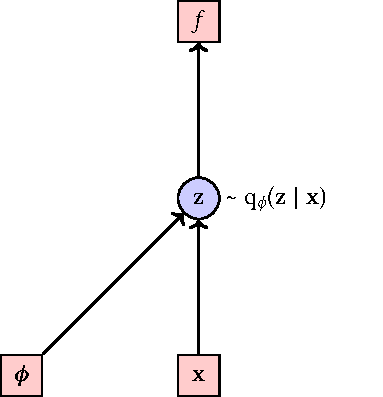
\includegraphics[height=7cm]{Appendix2/Figs/Vector/reparam_diagram.pdf}}
	\subfloat[Reparametrized]{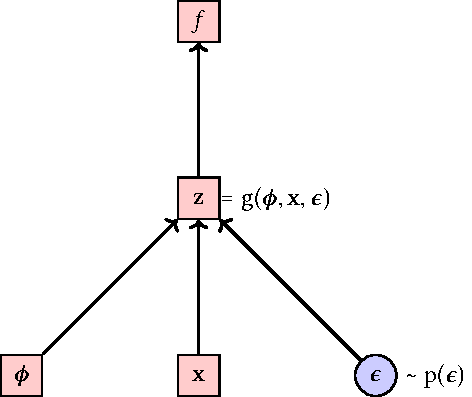
\includegraphics[height=7cm]{Appendix2/Figs/Vector/reparam_diagram2.pdf}}
	\caption[The reparametrization trick]{The reparametrization trick, adapted from~\cite{kingma2017variational}. The stochasticity of the $\mathbf{z}$ node is pushed out into a separate input to the same node, resulting in deterministic gradients w.r.t $\boldsymbol{\phi}$ through the node.}
	\label{fig:reparam}
\end{figure}
This was the gradient estimator originally used in the VAE implementation~\cite{kingma2013auto} there named as the \emph{reparametrization trick}, see also Figure~\ref{fig:reparam}. In many cases the transformation paths are so simple they can be implemented in one line of code, referred to as \emph{one-liners}. The pathwise-estimator can only be used on differentiable cost functions, but is easy to implement and crucially has lower variance than the score-function estimator.

\subsubsection{Measure-valued gradient estimator}
Which exploits the properties of signed-measures, is beyond the scope of this report.	

\section{Automatic differentiation}
\label{subsec:gbopt-autograd}

\section[\emph{Qptimal sampling}]{\emph{Qptimal sampling}: optimal sampling in lattice models}
\begin{figure}[h]
	\centering
	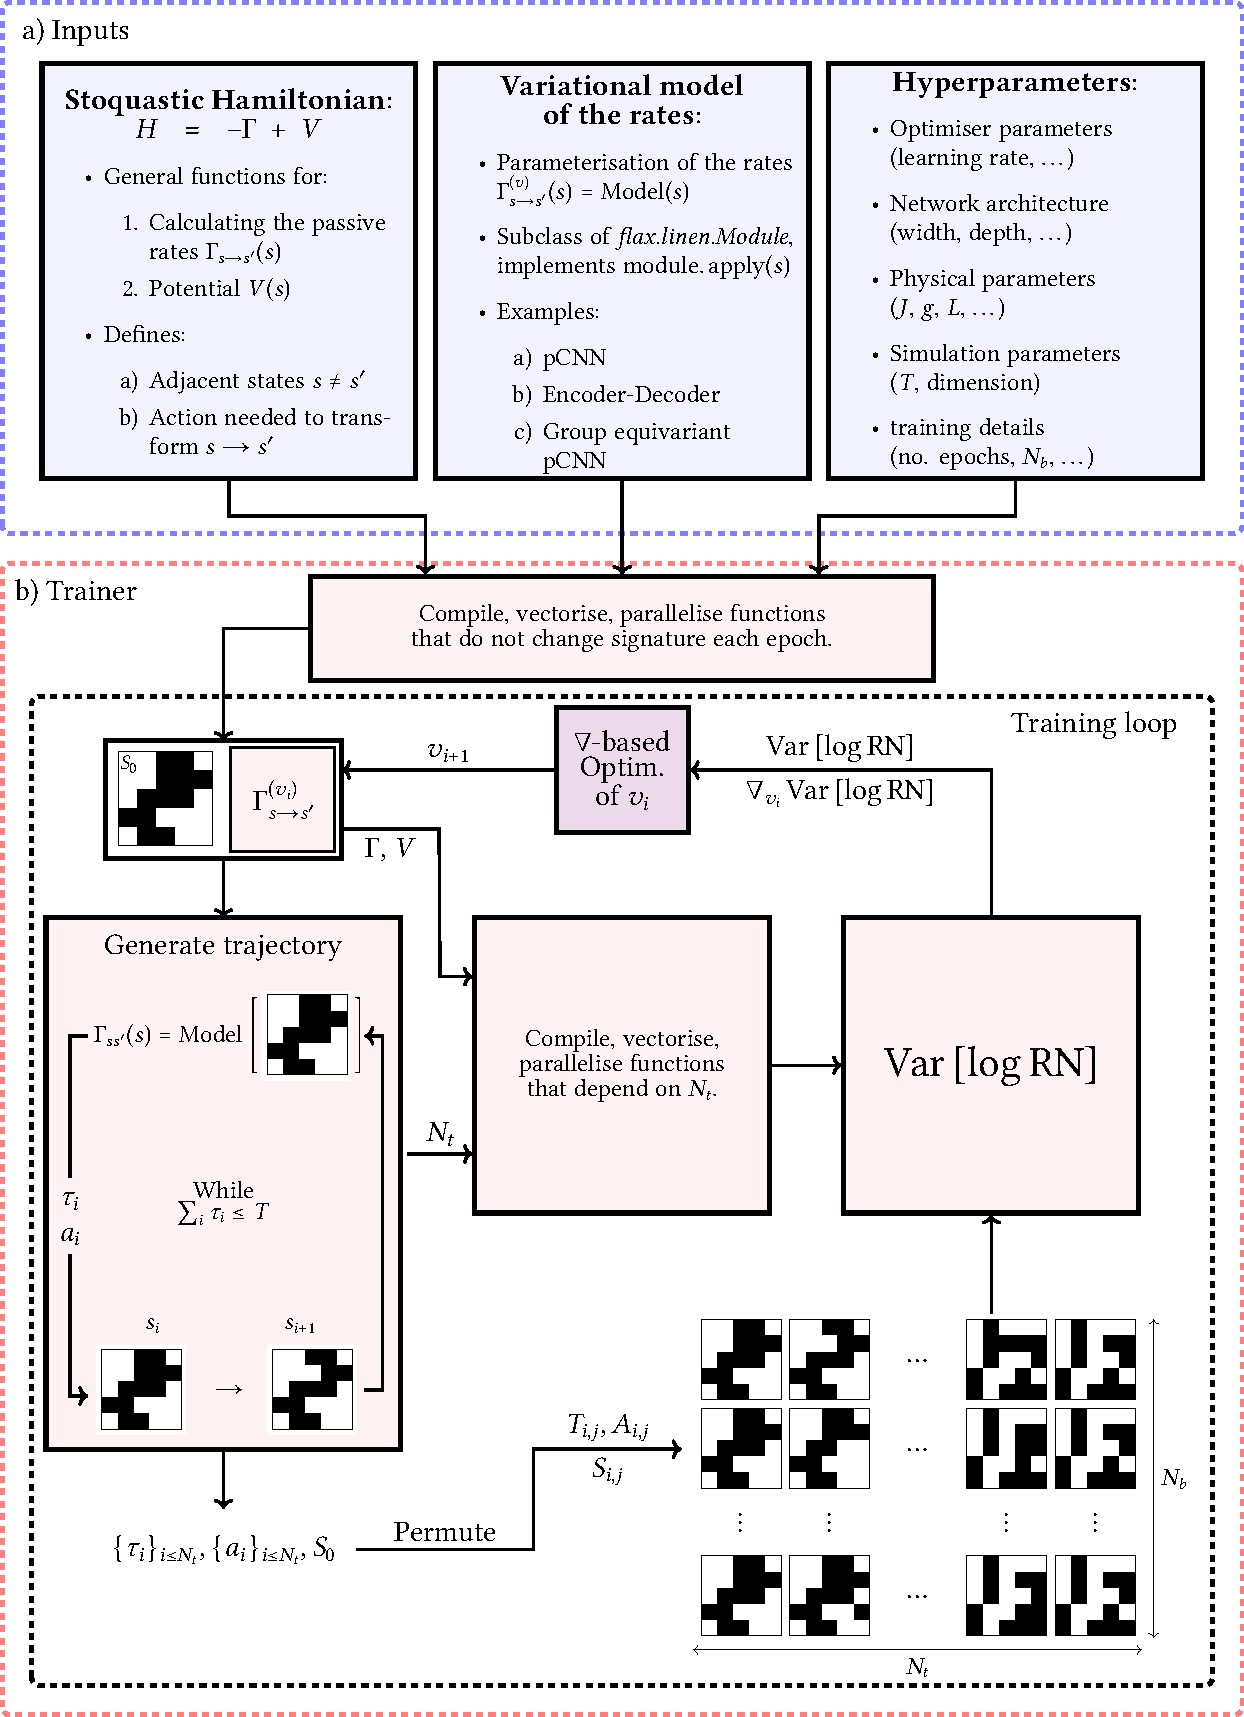
\includegraphics[width=\linewidth]{Chapter4/Figs/Vector/qsampl1}
\end{figure}
\begin{figure}[t]
	\ContinuedFloat
	\centering
	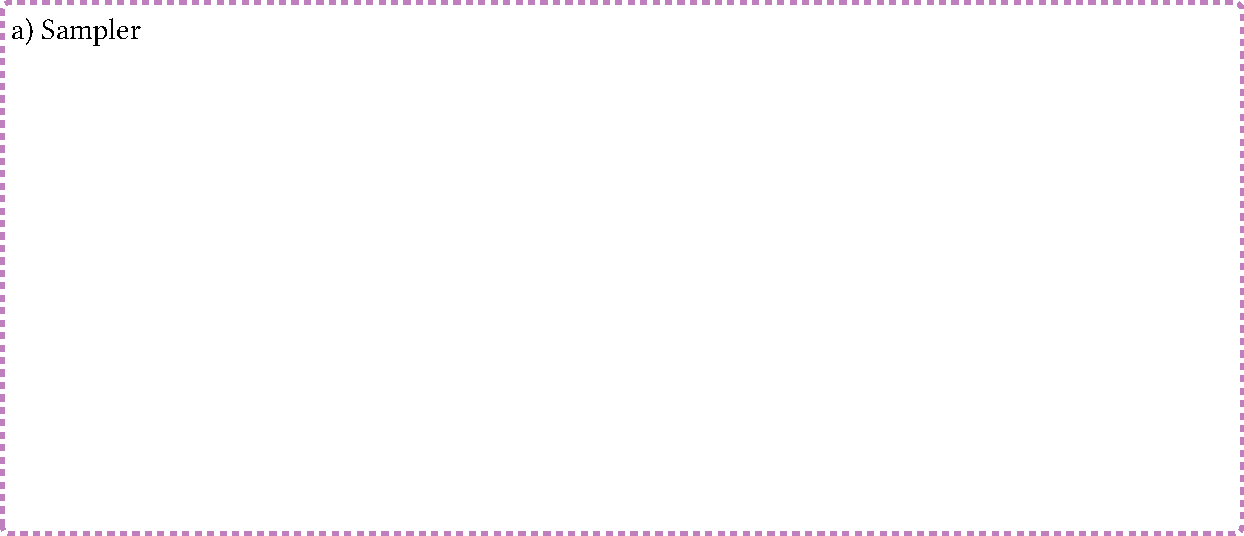
\includegraphics[width=\linewidth]{Chapter4/Figs/Vector/qsampl2}
	\caption[Implementation details]{\textbf{Implementation details}}
	\label{fig:qsampl}
\end{figure}



\subsection{Similarities to Score-Based models}
%!TEX root = ../thesis.tex
% **************************** Define Graphics Path **************************
\ifpdf
\graphicspath{{Chapter5/Figs/Raster/}{Chapter5/Figs/PDF/}{Chapter5/Figs/}}
\else
\graphicspath{{Chapter5/Figs/Vector/}{Chapter5/Figs/}}
\fi

%*******************************************************************************
%****************************** Fifth Chapter *********************************
%*******************************************************************************

\chapter{Experiments and Results}
\label{chapter5}
\hl{todo}
\begin{enumerate}
	\item training experiments
	\item sampling experiments
\end{enumerate}

\section{Learning the rates} 
\begin{figure}
	\centering
	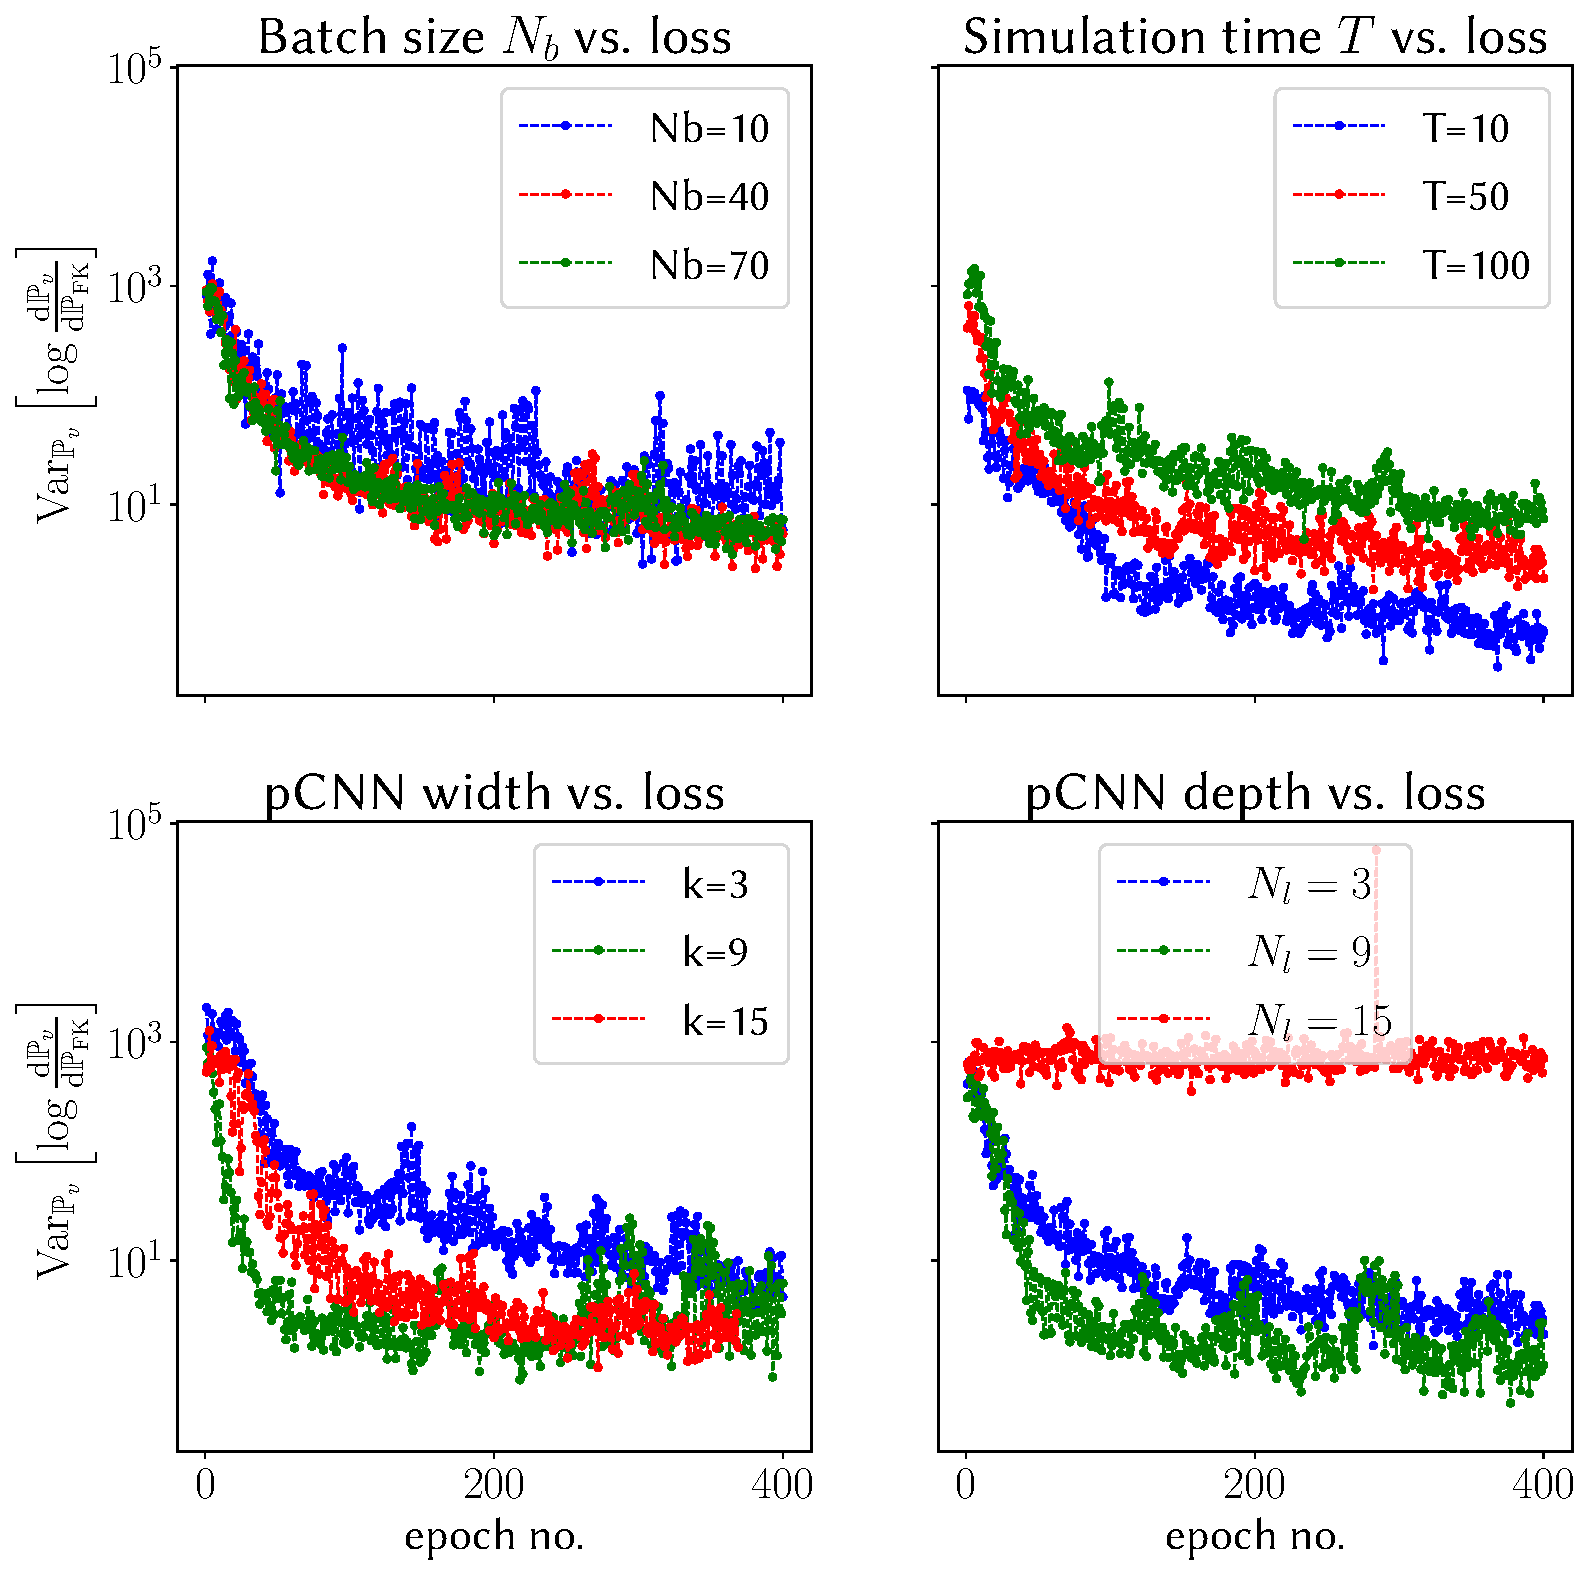
\includegraphics[width=\linewidth]{Chapter5/Figs/Vector/init_test_learning}
	\caption[Initial rate training experiments]{\textbf{Initial rate training experiments}}
	\label{fig:inittestlearning}
\end{figure}

\begin{figure}
	\centering
	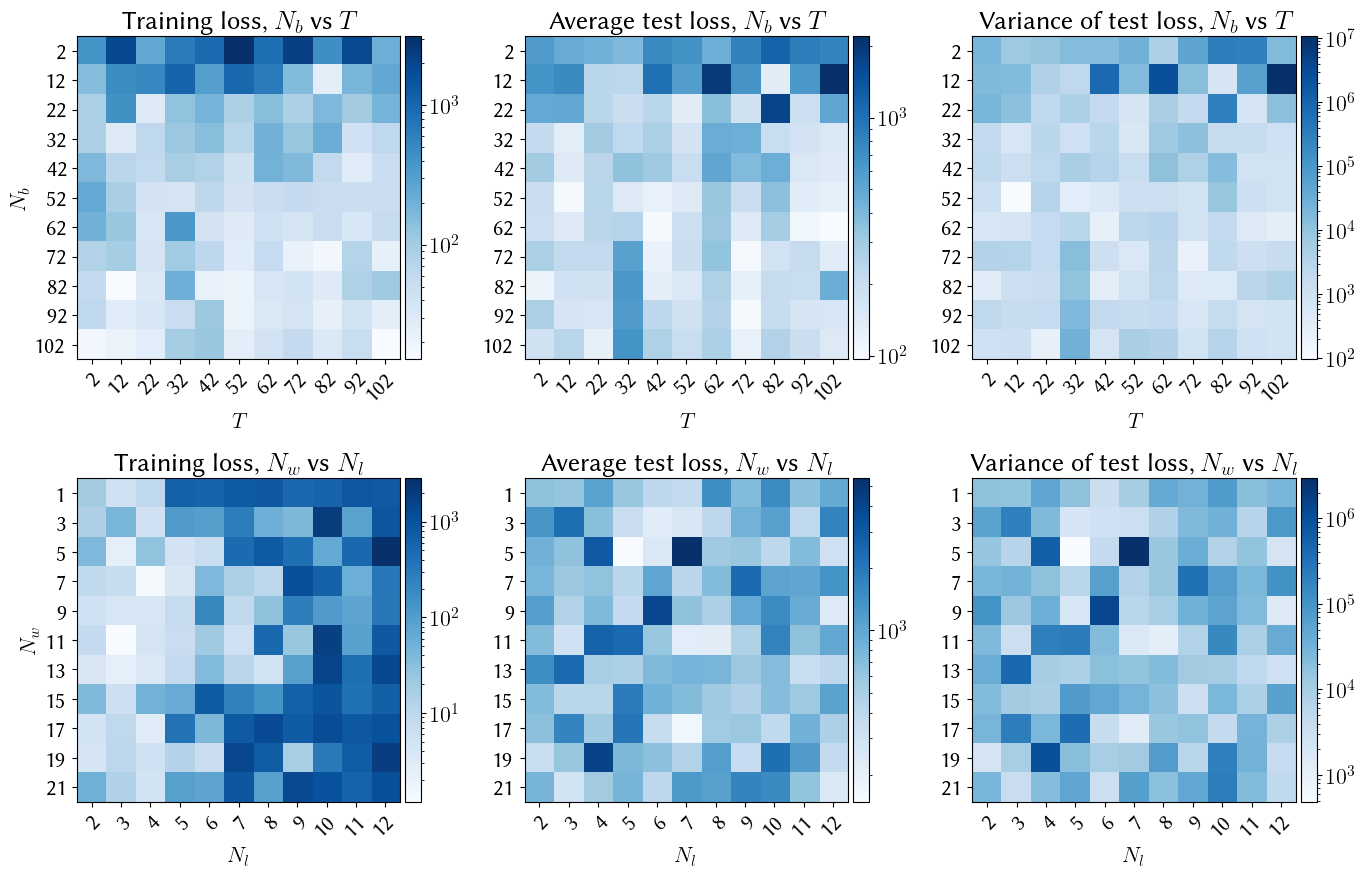
\includegraphics[width=\linewidth]{Chapter5/Figs/Raster/avg_var_loss}
	\caption[Performance of the pCNN for different setups]{\textbf{Performance of the pCNN for different setups.}}
	\label{fig:avgvarloss}
\end{figure}

\begin{figure}
	\centering
	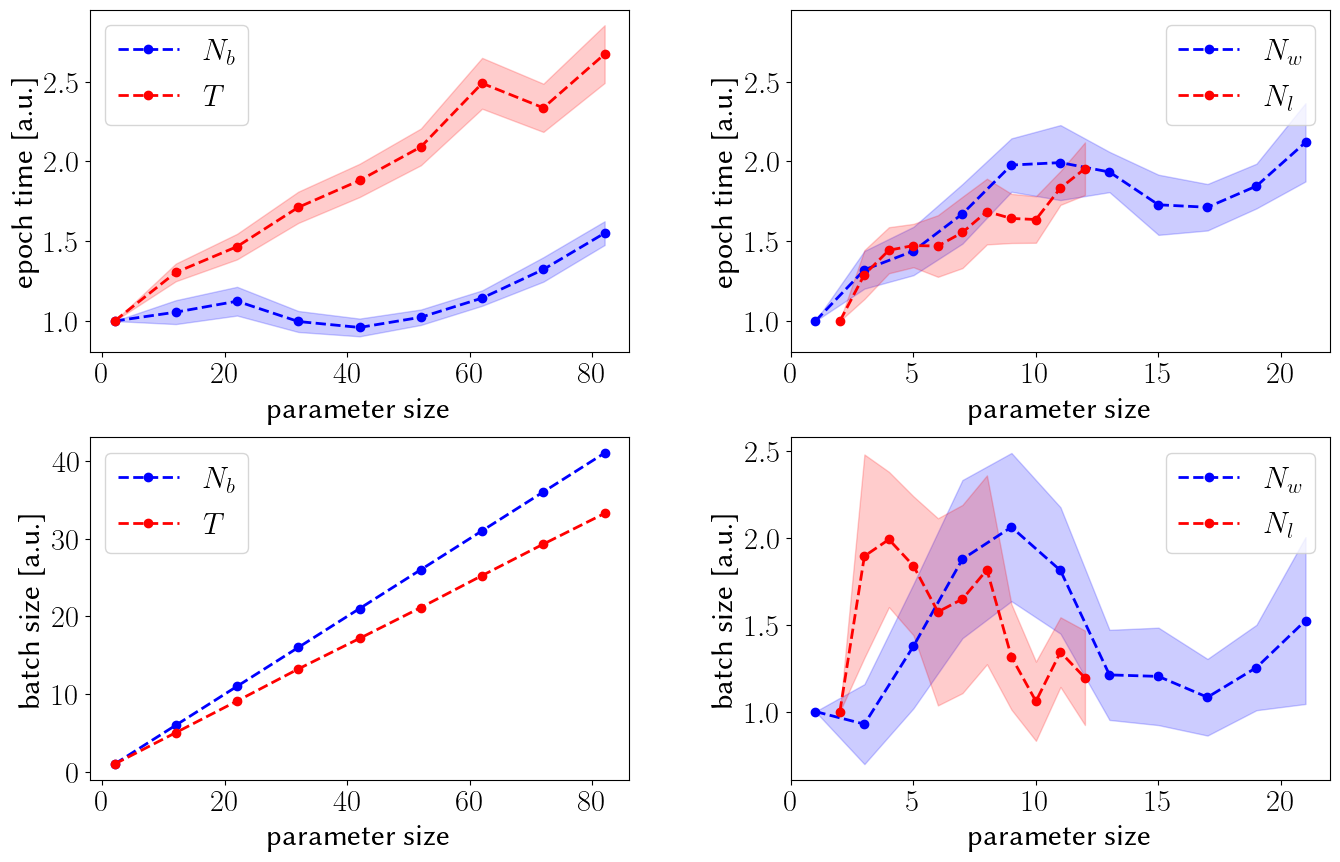
\includegraphics[width=\linewidth]{Chapter5/Figs/Raster/initial_time_space}
	\caption[Time and space complexity of the pCNN]{\textbf{Time and space complexity of the pCNN}}
	\label{fig:initialtimespace}
\end{figure}

%\subsubsection{How does simulation time $T$ and batch size $N_b$ affect the learning of the rates?}
%
%\subsubsection{How do architectural choices of the pCNN limit learning the rates?}
%
%\subsubsection{How does the size of lattice play a role?}
%
%\subsubsection{Can we improve learning by scaling the output of the pCNN?}
%Also mention reshuffling.
%
%\subsubsection{What role does symmetry play in all of this?}

\section{Importance sampling}
\section{Results}
\subsection{Ising model}
\subsubsection{One dimension}
\begin{figure}[H]
	\centering
	\subfloat[$E_0/N$]{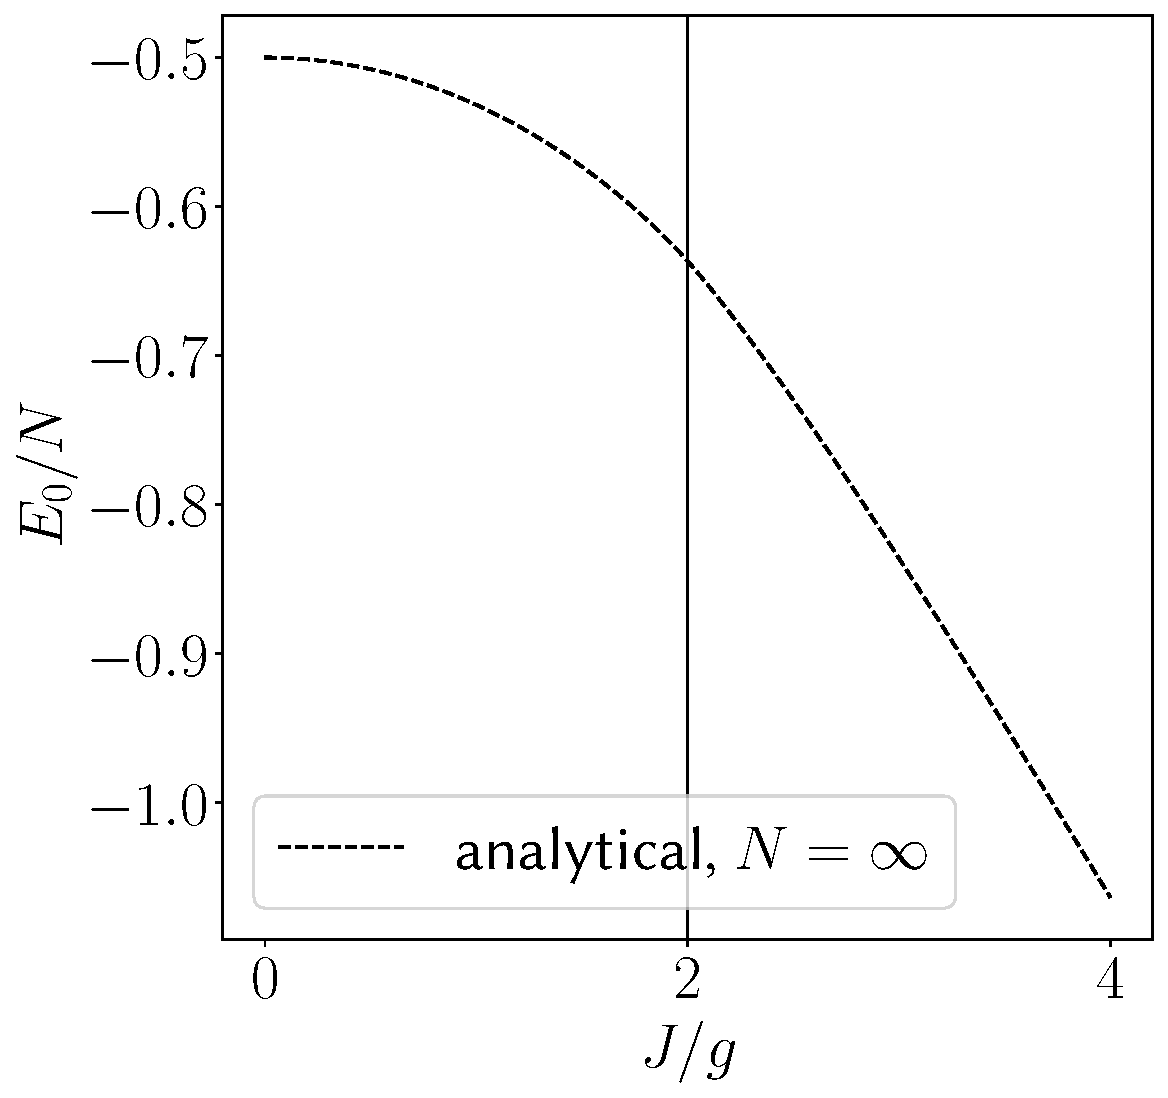
\includegraphics[width=0.345\linewidth]{Chapter5/Figs/Vector/tfim1d_en_finite_scaling.pdf}}
	\subfloat[$\sigma_z$]{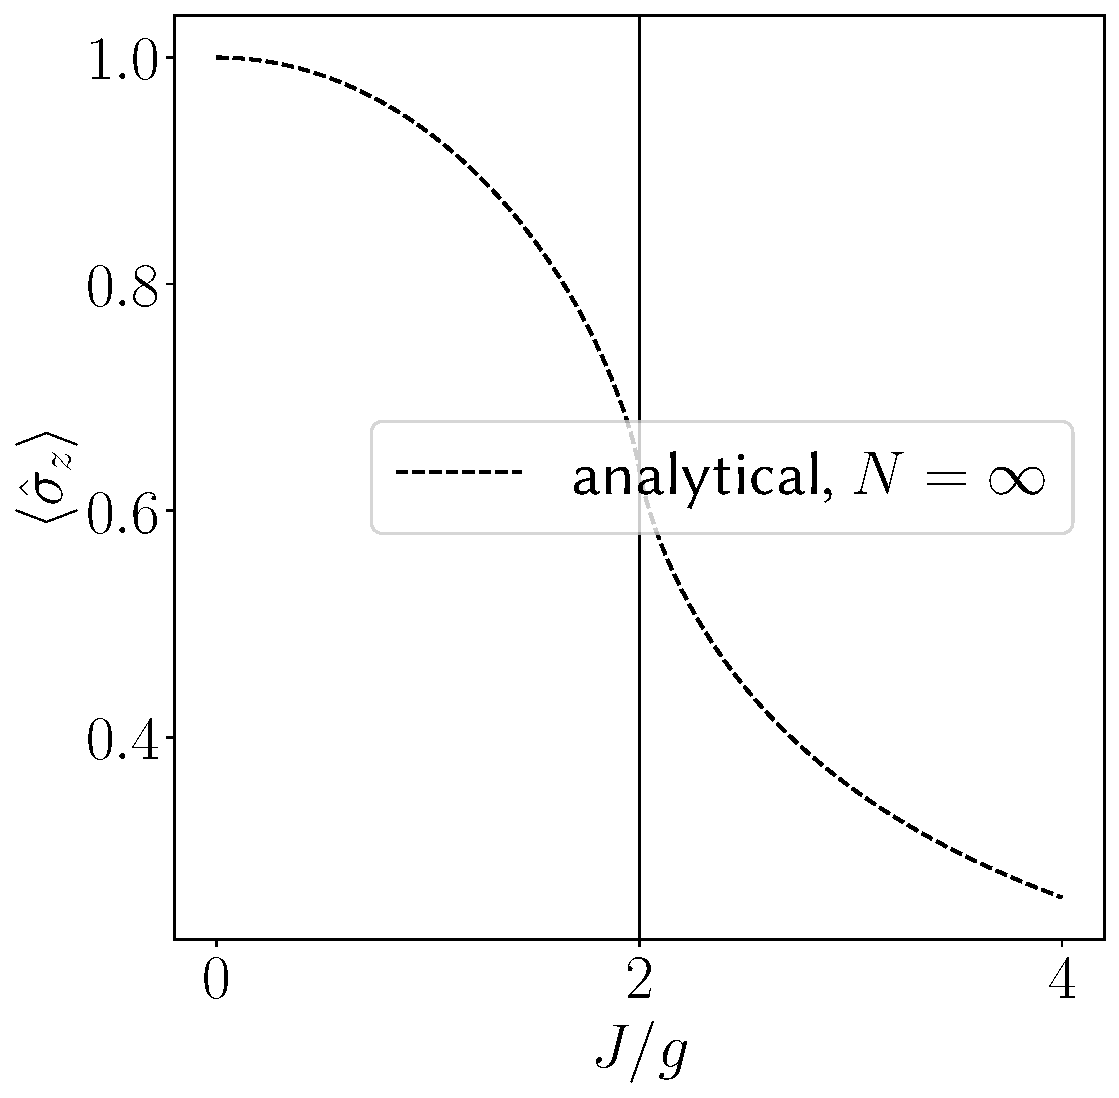
\includegraphics[width=0.33\linewidth]{Chapter5/Figs/Vector/tfim1d_mz_finite_scaling.pdf}}
	\subfloat[$\sigma_x$]{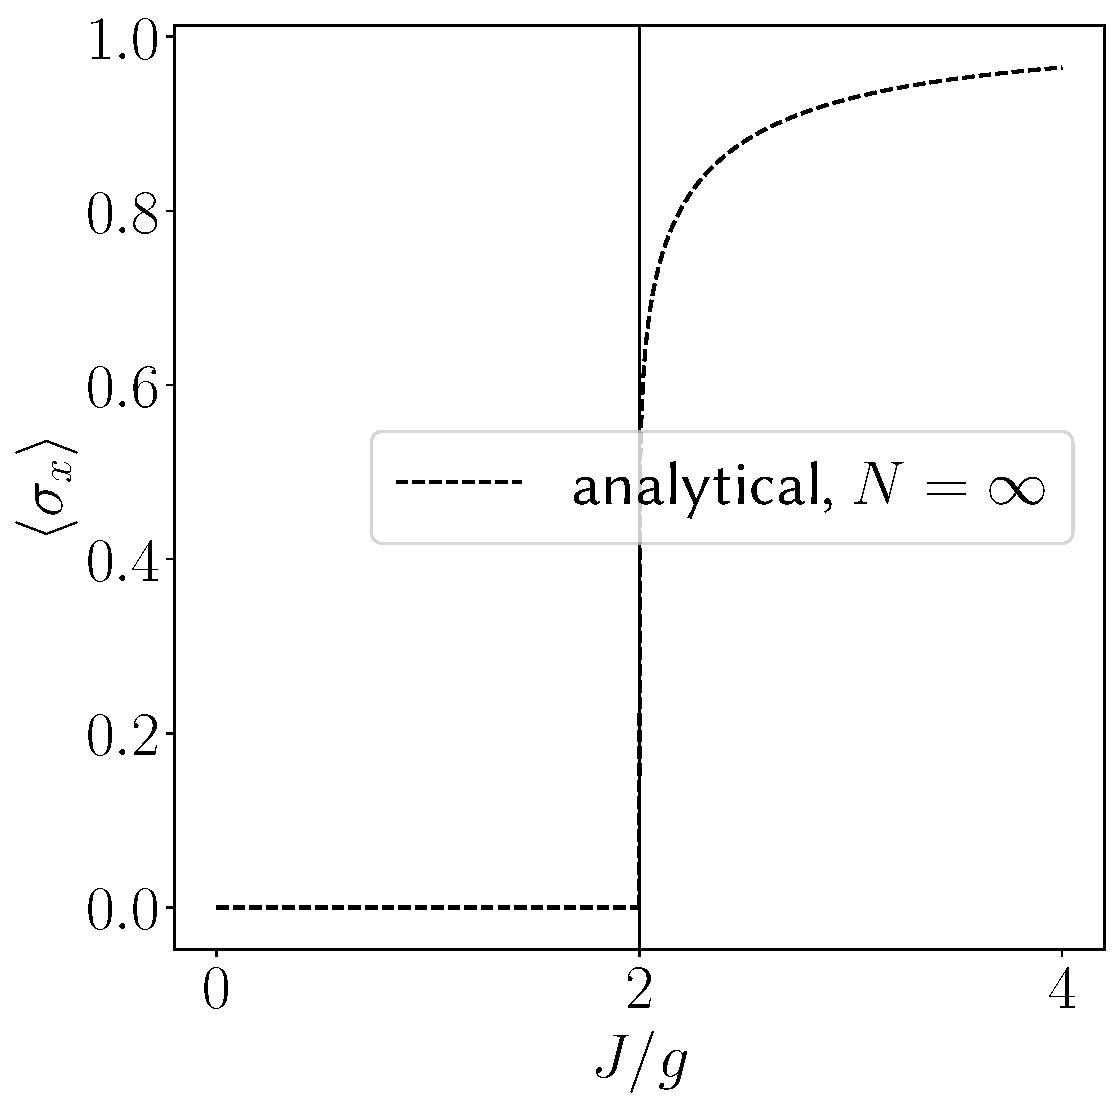
\includegraphics[width=0.33\linewidth]{Chapter5/Figs/Vector/tfim1d_mx_finite_scaling.pdf}}
	\caption[TFIM-1d energy and magnetisation]{\textbf{TFIM-1d energy and magnetisation}}
	\label{fig:tfim1d_finite_scaling_properties}
\end{figure}

\subsection{XY model}


%\begin{figure}[H]
%	\centering
%	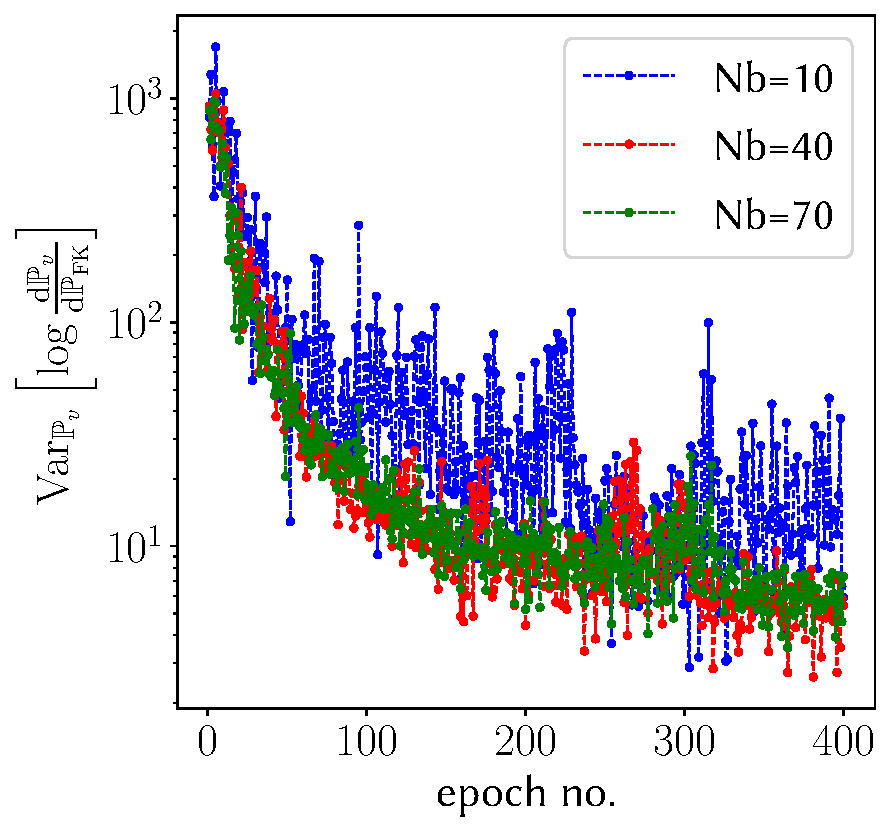
\includegraphics[width=\linewidth]{Chapter6/Figs/Vector/bvl_single}
%	\caption[Effect of batch size $N_b$ on training with the endpoint loss.]{\textbf{Effect of batch size $N_b$ on training with the endpoint loss.}}
%	\label{fig:bvlsingle}
%\end{figure}
%\begin{figure}[H]
%	\centering
%	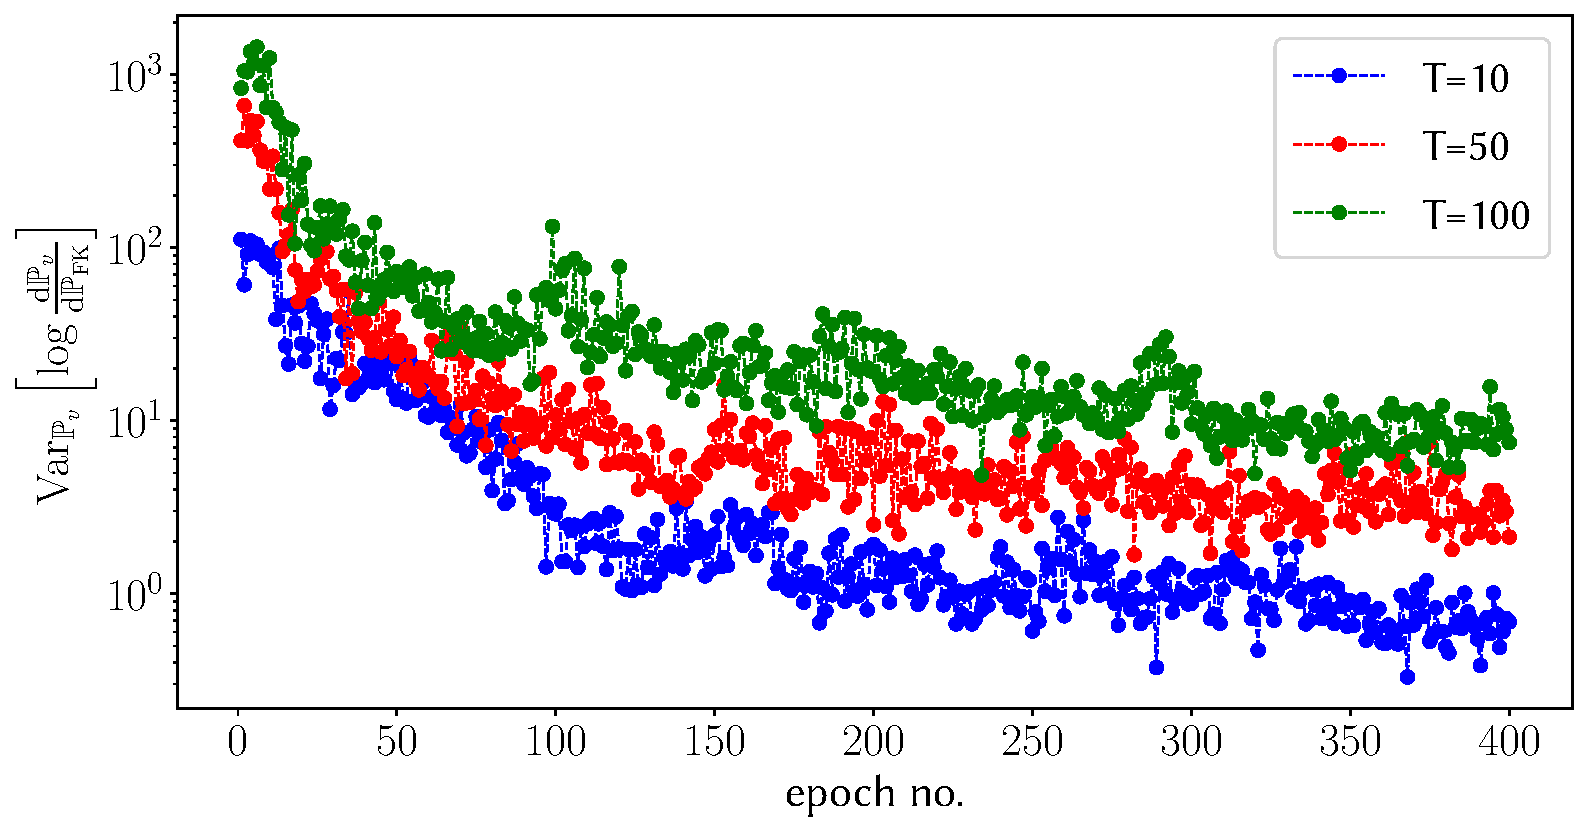
\includegraphics[width=\linewidth]{Chapter6/Figs/Vector/tvl_single}
%	\caption[Effect of simulation time $T$ on training with the endpoint loss.]{\textbf{Effect of simulation time $T$ on training with the endpoint loss.}}
%	\label{fig:tvlsingle}
%\end{figure}
%\begin{figure}[H]
%	\centering
%	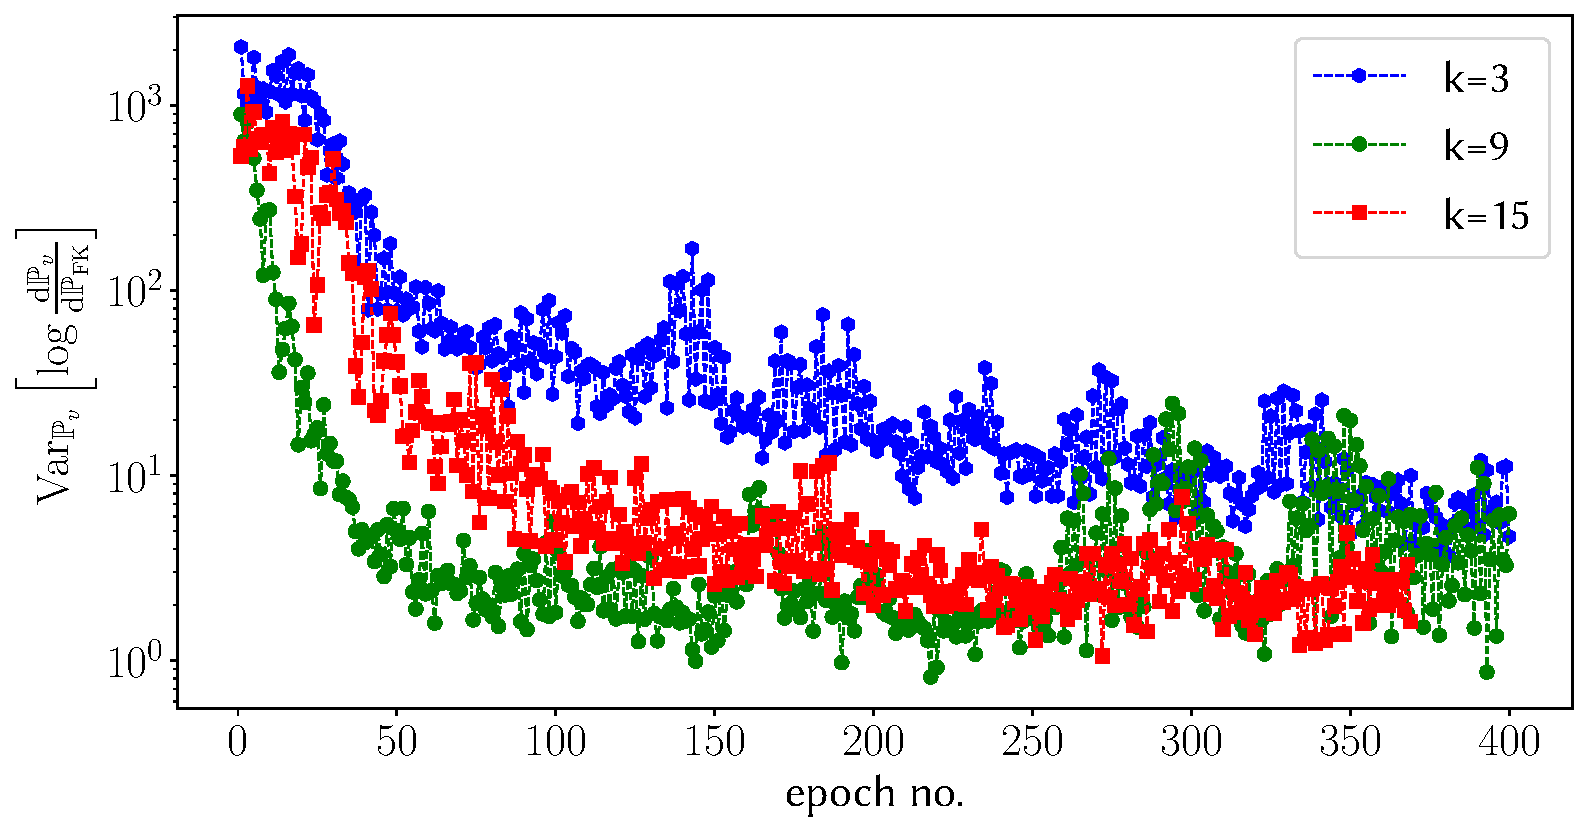
\includegraphics[width=\linewidth]{Chapter6/Figs/Vector/wvl_single}
%	\caption[Effect of pCNN width $k$ on training with the endpoint loss.]{\textbf{Effect of pCNN width $k$ on training with the endpoint loss.}}
%	\label{fig:wvlsingle}
%\end{figure}
%\begin{figure}[H]
%	\centering
%	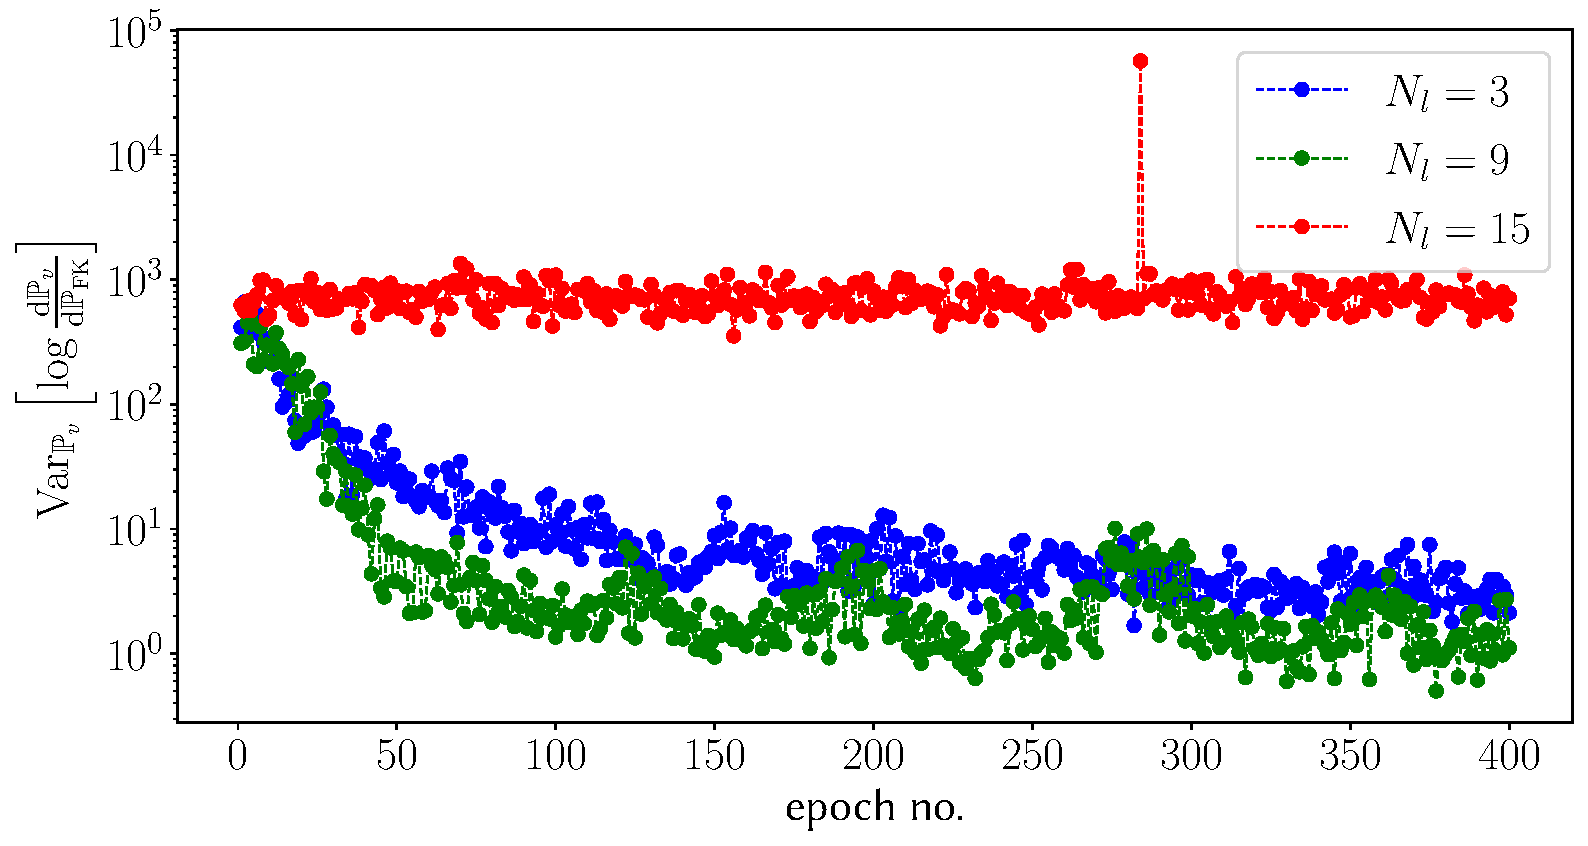
\includegraphics[width=\linewidth]{Chapter6/Figs/Vector/lvl_single}
%	\caption[Effect of pCNN depth $l$ on training with the endpoint loss.]{\textbf{Effect of pCNN depth $l$ on training with the endpoint loss.}}
%	\label{fig:lvlsingle}
%\end{figure}
%!TEX root = ../thesis.tex
%*******************************************************************************
%****************************** Fifth Chapter **********************************
%*******************************************************************************

\chapter{Results}
\label{chapter6}

% **************************** Define Graphics Path **************************
\ifpdf
\graphicspath{{Chapter5/Figs/Raster/}{Chapter5/Figs/PDF/}{Chapter5/Figs/}}
\else
\graphicspath{{Chapter5/Figs/Vector/}{Chapter5/Figs/}}
\fi

\subsection{Single Particle on a Lattice}
\begin{equation}
	\partial_{t} \psi_{j}=\frac{1}{2}\left[\psi_{j+1}+\psi_{j-1}-2 \psi_{j}\right]+V_{j} \psi_{j}
\end{equation}

\begin{equation}
	\psi_{j}(t)=\underset{X \sim \mathrm{SRW} \text { with } X_{t}=j}{\mathbb{E}} \left[\exp \left(-\int_{0}^{t}  V\left(X_{\tau}, \tau\right) \mathrm{d} \tau \right) \psi_{X_{0}}(0)\right]
\end{equation}

\section{Transverse-field Ising model}
\label{sec:res-im}

\section{Heisenberg model}
\label{sec:res-hm}

Heisenberg ferromagnet
\begin{equation}
	\hat H_{\mathrm{F}}=-\frac{1}{2} \sum_{j}\left[\hat{\sigma}_{j}^{x} \hat{\sigma}_{j+1}^{x}+\hat{\sigma}_{j}^{y} \hat{\sigma}_{j+1}^{y}+\hat{\sigma}_{j}^{z} \hat{\sigma}_{j+1}^{z}\right]
\end{equation}

The XY model.
\begin{equation}
	\begin{aligned} 
		\hat H_{X Y}=-\sum_{j}\left[\hat{\sigma}_{j}^{x} \hat{\sigma}_{j+1}^{x}+\hat{\sigma}_{j}^{y} \hat{\sigma}_{j+1}^{y}\right] &=H_{\mathrm{F}}+\frac{1}{2} \sum_{j} \hat{\sigma}_{j}^{z} \hat{\sigma}_{j+1}^{z} \\ 						&=-\mathcal{W}+\sum_{j}\left[n_{j}\left(1-n_{j+1}\right)+n_{j+1}\left(1-n_{j}\right)\right] 
	\end{aligned}
\end{equation}

\begin{equation}
	\psi_{s_{1: N}}(t)=\underset{\Sigma_{[0, t]} \sim \operatorname{SEP} \text{ with } \Sigma_{t}=s_{1: N}}{\mathbb{E}}
	\left[\exp \left(-\int_{0}^{t} d t^{\prime} \sum_{j}\left[n_{j}\left(1-n_{j+1}\right)+n_{j+1}\left(1-n_{j}\right)\right]\right) \psi_{\Sigma_{0}}(0)\right]
\end{equation}

\section{Bose-Hubbard model}
\label{sec:res-bhm}





%%!TEX root = ../thesis.tex
%*******************************************************************************
%****************************** Third Chapter **********************************
%*******************************************************************************

\chapter{Conclusions}
\label{chapter7}

% **************************** Define Graphics Path **************************
\ifpdf
    \graphicspath{{Chapter7/Figs/Raster/}{Chapter7/Figs/PDF/}{Chapter7/Figs/}}
\else
    \graphicspath{{Chapter7/Figs/Vector/}{Chapter7/Figs/}}
\fi

\section{Direction for further work}

\section{Remarks}



% ********************************** Back Matter *******************************
% Backmatter should be commented out, if you are using appendices after References
%\backmatter

% ********************************** Bibliography ******************************
\begin{spacing}{0.9}

% To use the conventional natbib style referencing
% Bibliography style previews: http://nodonn.tipido.net/bibstyle.php
% Reference styles: http://sites.stat.psu.edu/~surajit/present/bib.htm

\bibliographystyle{apalike}
%\bibliographystyle{unsrt} % Use for unsorted references  
%\bibliographystyle{plainnat} % use this to have URLs listed in References
\cleardoublepage
\bibliography{References/references} % Path to your References.bib file


% If you would like to use BibLaTeX for your references, pass `custombib' as
% an option in the document class. The location of 'reference.bib' should be
% specified in the preamble.tex file in the custombib section.
% Comment out the lines related to natbib above and uncomment the following line.

%\printbibliography[heading=bibintoc, title={References}]


\end{spacing}

% ********************************** Appendices ********************************

\begin{appendices} % Using appendices environment for more functunality

%!TEX root = ../thesis.tex
% ******************************* Thesis Appendix A ****************************
\chapter{Jax ecosystem} 

%%!TEX root = ../thesis.tex
% ******************************* Thesis Appendix B ********************************

\chapter{Gradient estimation}
\label{app:grad_estim}
In order to perform gradient descent on the ELBO objective, we need to be able to evaluate its gradients with respect to parameters $\boldsymbol{\theta}$ and $\boldsymbol{\phi}$. Taking the gradient w.r.t generative parameters $\boldsymbol{\theta}$ is straightforward, because we can change the order of the expectation operator and the gradient, leaving us with
\begin{equation}
	\begin{aligned} 
		\nabla_{\boldsymbol{\theta}} \mathcal{L}_{\boldsymbol{\theta}, \boldsymbol{\phi}}(\mathbf{x}) &=\nabla_{\boldsymbol{\theta}} 	\mathbb{E}_{q_{\boldsymbol{\phi}}(\mathbf{z} \mid \mathbf{x})}\left[\log p_{\boldsymbol{\theta}}(\mathbf{x}, \mathbf{z})-\log q_{\boldsymbol{\phi}}(\mathbf{z} | \mathbf{x})\right] \\  & \simeq \nabla_{\boldsymbol{\theta}}\left(\log p_{\boldsymbol{\theta}}(\mathbf{x}, \mathbf{z})-\log q_{\boldsymbol{\phi}}(\mathbf{z} | \mathbf{x})\right) \\ &=\nabla_{\boldsymbol{\theta}}\left(\log p_{\boldsymbol{\theta}}(\mathbf{x}, \mathbf{z})\right) ,
	\end{aligned}
\end{equation}
where $\simeq$ denotes an unbiased estimator. This reversing of the order of operations is not possible when taking gradients w.r.t variational parameters $\boldsymbol{\phi}$ because the expectation $\mathbb{E}_{q_{\boldsymbol{\phi}}(\mathbf{z} | \mathbf{x})}$ is performed w.r.t the approximate posterior $q_{\boldsymbol{\phi}}(\mathbf{z} | \mathbf{x})$. The gradient could be estimated with a vanilla Monte Carlo estimator, but it has very high variance and is not practical~\cite{kingma2013auto}. 

The problem of stochastic gradient estimation of an expectation of a function is a well studied problem that transcends machine learning and has a variety of applications~\cite{chriss1997black, schrittwieser2020mastering}. Different estimators differ in from and their properties, variance being one of the most important. In their review~\cite{mohamed2020monte} Mohamed et al. categorise MC gradient estimators into three categories
\begin{enumerate}
	\item \emph{Score-function estimator}: The score function is a logarithm of a probability distribution w.r.t to distributional parameters. It can be used as a gradient estimator
	\begin{equation}
		\begin{aligned}
			\nabla_{\boldsymbol{\theta}} \mathbb{E}_{p_{\boldsymbol{\theta}}(\mathbf{x})}[f(\mathbf{x})] &=  \nabla_{\boldsymbol{\theta}} \int p_{\boldsymbol{\theta}}(\mathbf{x}) f(\mathbf{x}) d \mathbf{x} \\
			&= \mathbb{E}_{p_{\boldsymbol{\theta}}(\mathbf{x})}\left[f(\mathbf{x}) \nabla_{\boldsymbol{\theta}} \log p_{\boldsymbol{\theta}}(\mathbf{x})\right].
		\end{aligned}
	\end{equation}
	The score-function estimator is compatible with any cost function, it requires that the measure $p_{\boldsymbol{\theta}}(\mathbf{x})$ is differentiable and easy to sample. Very importantly it is applicable to both discrete and continuous distribution, but has a drawback of having high variance.
	
	\item \emph{Pathwise estimator}: Continuous distributions can be sampled either directly by generating samples from the distribution $p_{\boldsymbol{\theta}}(\mathbf{x})$ or indirectly, by sampling from a simpler base distribution $p(\boldsymbol{\epsilon})$ and transforming the variate through a deterministic path $g_{\boldsymbol{\theta}}(\boldsymbol{\epsilon})$. Using this, it is possible to move the source of randomness in such a way that the objective is differentiable. In essence this approach pushes the parameters of the measure into the cost function which is then differentiated. The estimator is
	\begin{equation}
		\begin{aligned}
			\nabla_{\boldsymbol{\theta}} \mathbb{E}_{p_{\boldsymbol{\theta}}(\mathbf{x})}[f(\mathbf{x})] 
			&=\nabla_{\boldsymbol{\theta}} \int p_{\boldsymbol{\theta}}(\mathbf{x}) f(\mathbf{x}) d \mathbf{x} \\
			&= \nabla_{\boldsymbol{\theta}} \int p(\boldsymbol{\epsilon}) f(g_{\boldsymbol{\theta}}(\boldsymbol{\epsilon})) d \boldsymbol{\epsilon} \\
			&= \mathbb{E}_{p(\boldsymbol{\epsilon})}\left[\nabla_{\boldsymbol{\theta}} f(g_{\boldsymbol{\theta}}(\boldsymbol{\epsilon}))\right].
		\end{aligned}
	\end{equation}
	\begin{figure}
		\centering
		\subfloat[Original]{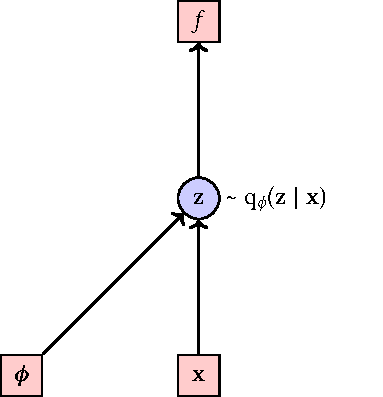
\includegraphics[height=7cm]{Appendix2/Figs/Vector/reparam_diagram.pdf}}
		\subfloat[Reparametrized]{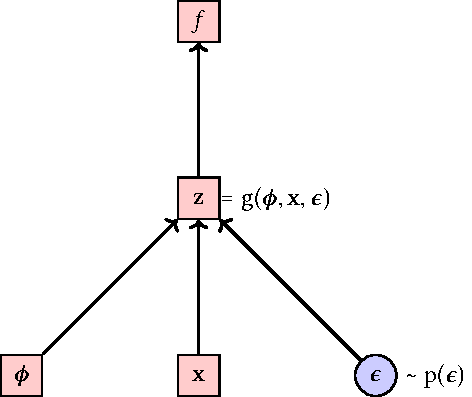
\includegraphics[height=7cm]{Appendix2/Figs/Vector/reparam_diagram2.pdf}}
		\caption[The reparametrization trick]{The reparametrization trick, adapted from~\cite{kingma2017variational}. The stochasticity of the $\mathbf{z}$ node is pushed out into a separate input to the same node, resulting in deterministic gradients w.r.t $\boldsymbol{\phi}$ through the node.}
		\label{fig:reparam}
	\end{figure}
	This was the gradient estimator originally used in the VAE implementation~\cite{kingma2013auto} there named as the \emph{reparametrization trick}, see also Figure~\ref{fig:reparam}. In many cases the transformation paths are so simple they can be implemented in one line of code, referred to as \emph{one-liners}. The pathwise-estimator can only be used on differentiable cost functions, but is easy to implement and crucially has lower variance than the score-function estimator. 
	
	\item \emph{Measure-valued gradient estimator}, which exploits the properties of signed-measures, is beyond the scope of this report.	
\end{enumerate}
Unbiased gradient estimation makes training on the ELBO objective possible. During training the VAE learns a mapping between a complicated observed space of $\mathbf{x}$ and the latent space of $\mathbf{z}$, which is usually defined to be relatively simple. The \emph{decoder} network or the \emph{generative} part of the VAE $p_{\boldsymbol{\theta}}(\mathbf{x} | \mathbf{z})$ learns to map from the latent space to the data space, while the \emph{inference} or \emph{encoder} network $q_{\mathbf{\phi}}(\mathbf{z}|\mathbf{x})$ approximates the true posterior $p_{\mathbf{\theta}}(\mathbf{z}|\mathbf{x})$ of this process, see Figure. 


%%!TEX root = ../thesis.tex
% ******************************* Thesis Appendix C ********************************

\chapter{Additional results}

%%!TEX root = ../thesis.tex
% ******************************* Thesis Appendix C ********************************

\chapter{Additional Derivations}


\end{appendices}

% *************************************** Index ********************************
\printthesisindex % If index is present

\end{document}
